\documentclass[a4paper, 12pt, twoside]{report}


%%% Language
\usepackage[english]{babel}
%\usepackage[ngerman]{babel}


%%% Encoding
\usepackage[latin1]{inputenc}   % Linux / UNIX
% \usepackage[ansinew]{inputenc}  % Windows
% \usepackage[utf8]{inputenc}     % UTF8


%%% Packages (add new as needed)
%\usepackage{graphicx}           % include graphics
\usepackage[pdftex]{graphicx}
\usepackage{amsmath}            % nice equations
\usepackage{url}                % URLs
%\usepackage{natbib}             % author-year bibliography style
\usepackage{cite}
\usepackage{baithesis}          % BAI thesis
\usepackage{pdfpages}
\usepackage{float}
\usepackage{subfig}
\usepackage{grffile}
%\usepackage[square]{natbib}
\usepackage{natbib}
\usepackage[acronym, nonumberlist]{glossaries}
\usepackage{copyrightbox}

\numberwithin{equation}{section}
\providecommand{\keywords}[1]{\textbf{\textit{Keywords---}} #1}

\makeglossaries
\newacronym{fmri}{fMRI}{functional magnetic resonance imaging}
\newacronym{fnirs}{fNIRS}{functional near-infrared spectroscopy}
\newacronym{cw-nirs}{CW-NIRS}{continuous wave near-infrared spectroscopy}
\newacronym{fd-nirs}{FD-NIRS}{frequency domain near-infrared spectroscopy}
\newacronym{td-nirs}{TD-NIRS}{time domain near-infrared spectroscopy}
\newacronym{dpf}{DPF}{differential path length factor}
\newacronym{sts}{STS}{superior temporal sulcus}
\newacronym{HbR}{HbR}{deoxygenated hemoglobin}
\newacronym{HbO}{HbO}{oxygenated hemoglobin}
\newacronym{sci}{SCI}{scalp coupling index}
\newacronym{icra}{ICRA}{International Collegium for Rehabilitative Audiology}
\newacronym{bold}{BOLD}{blood-oxygen-level-dependent}
\newacronym{mbll}{mBLL}{modified Beer-Lambert law}
\newacronym{pca}{PCA}{principle component analysis}
\newacronym{lsl}{LSL}{lab streaming layer}
\newacronym{prs}{PRS}{phase-resolved spectroscopy}
\newacronym{glm}{GLM}{general linear model}
\newacronym{roi}{ROI}{region of interest}
\newacronym{spl}{SPL}{sound pressure level}

%\usepackage{ngerman}
\usepackage{hyperref}           % PDF links
% \usepackage{subfig}             % Subfigures (a), (b), etc
% \usepackage{nomencl}            % Nomenclature

%%% Meta data
\author{Pei-Yi Lin}
\title{Investigation of Cortical Responses to Modulated Noise Stimuli Using fNIRS}
\date{\today}
%\degree{Bachelorarbeit}
\supervisors{Prof.\ Dr.-Ing.\ Werner Hemmert\\
  Dr. \ Ali Saeedi \\
  M.Sc.\ Carmen Marie Casta\~{n}eda Gonz\'{a}lez}
\logo{bai-tum}


%%%%%%%%%%%%%%%%%%%%%%%%%%%%%%%%%%%%%%%%%%%%%%%%%%%%%%%%%%%%%%%%%%%%%%
%%%%%%%%%%%%%%%%%%%%%%%%%%%%% Document %%%%%%%%%%%%%%%%%%%%%%%%%
\begin{document}
%%% Title page
\pagenumbering{roman}
\maketitle{}


%%% Abstract
\begin{abstract}
In this study, we sought to determine whether \acrlong{fnirs} (\acrshort{fnirs}), a non-invasive neuroimaging method that is safe to use repeatedly and for an extended period of time, can provide an objective measure of the cortical response when subjects are exposed to different levels of sound intensity. Eight normal-hearing subjects, including both biological genders and different races, were included and actively participated in the present study. Measurement data were processed to compute the changes in oxyhemoglobin and deoxyhemoglobin concentration. The resulting waveform morphologies were studied and a regional analysis was conducted. The results were compared with previous studies, mainly the one from Weder et al. \citeyearpar{Weder2018}. Potential reasons to cause the variance from the previous research \citep{Weder2018} were investigated. The feasibility of using fNIRS for neuroimaging in hearing research was once again evaluated. \\
\newline

\keywords{ \acrlong{fnirs},	cortical responses,	sound intensities , language processing ,	normal-hearing listeners}

\end{abstract}



\cleardoublepage{}


%%% Acknowledgments (optional)
\begin{acknowledgments}
Huge thanks to my friends who volunteered and participated in this study.
\end{acknowledgments}


%%% Nomenclature (optional)
%%% Recommended to use: nomencl.sty
%%% Otherwise:
% \chapter*{Nomenclature}
% \input{example/abbrevs}


%%% Table of Contents

\cleardoublepage{}
\tableofcontents
\cleardoublepage{}
\pagenumbering{arabic}



%%% Chapters
%
\chapter{Example chapter of the thesis}
\label{cha:example-chapt-thes}

Some good tips:

\begin{itemize}
\item use \cite{Oetiket2008Short} as your reference
\item create seperate directory for your chapters, e.g.,
  \texttt{content}
\item in case of serious problems, ask Marek for help
\end{itemize}



\section{Beautiful table}
\label{sec:beautiful-table}

\begin{table}[htbp]
  \centering
  \begin{tabular}{c c c}
    \hline{}
    \textbf{Color} & \textbf{Shape} & \textbf{Area} \\
    \hline{}
    black & circle & 23 \\
    yellow & square & 43 \\
    red & triangle & 123 \\
    \hline{}
  \end{tabular}
  \caption{Very nice table of shapes and colors.}
  \label{tab:cute}
\end{table}



\section{Fake section}
\label{sec:fake-section}

Aasdf asdf asdf sadf sakldjf laskjflksajfd lkasjdflk asjdlkfj aslkdfj
aslkfsakhf sfjsaf jaslkfj asdf.  Aasdf asdf asdf sadf sakldjf
laskjflksajfd lkasjdflk asjdlkfj aslkdfj aslkfsakhf sfjsaf jaslkfj
asdf.  Aasdf asdf asdf sadf sakldjf laskjflksajfd lkasjdflk asjdlkfj
aslkdfj aslkfsakhf sfjsaf jaslkfj asdf.  Aasdf asdf asdf sadf sakldjf
laskjflksajfd lkasjdflk asjdlkfj aslkdfj aslkfsakhf sfjsaf jaslkfj
nnasdf.  Aasdf asdf asdf sadf sakldjf laskjflksajfd lkasjdflk asjdlkfj
aslkdfj aslkfsakhf sfjsaf jaslkfj asdf.  Aasdf asdf asdf sadf sakldjf
laskjflksajfd lkasjdflk asjdlkfj aslkdfj aslkfsakhf sfjsaf jaslkfj
asdf.  Aasdf asdf asdf sadf sakldjf laskjflksajfd lkasjdflk asjdlkfj
aslkdfj aslkfsakhf sfjsaf jaslkfj asdf.  Aasdf asdf asdf sadf sakldjf
laskjflksajfd lkasjdflk asjdlkfj aslkdfj aslkfsakhf sfjsaf jaslkfj
asdf.  Aasdf asdf asdf sadf sakldjf laskjflksajfd lkasjdflk asjdlkfj
aslkdfj aslkfsakhf sfjsaf jaslkfj asdf.



Aasdf asdf asdf sadf sakldjf laskjflksajfd lkasjdflk asjdlkfj aslkdfj
aslkfsakhf sfjsaf jaslkfj asdf.  Aasdf asdf asdf sadf sakldjf
laskjflksajfd lkasjdflk asjdlkfj aslkdfj aslkfsakhf sfjsaf jaslkfj
asdf.  Aasdf asdf asdf sadf sakldjf laskjflksajfd lkasjdflk asjdlkfj
aslkdfj aslkfsakhf sfjsaf jaslkfj asdf.  Aasdf asdf asdf sadf sakldjf
laskjflksajfd lkasjdflk asjdlkfj aslkdfj aslkfsakhf sfjsaf jaslkfj
asdf.  Aasdf asdf asdf sadf sakldjf laskjflksajfd lkasjdflk asjdlkfj
aslkdfj aslkfsakhf sfjsaf jaslkfj asdf.  Aasdf asdf asdf sadf sakldjf
laskjflksajfd lkasjdflk asjdlkfj aslkdfj aslkfsakhf sfjsaf jaslkfj
asdf.  Aasdf asdf asdf sadf sakldjf laskjflksajfd lkasjdflk asjdlkfj
aslkdfj aslkfsakhf sfjsaf jaslkfj asdf.  Aasdf asdf asdf sadf sakldjf
laskjflksajfd lkasjdflk asjdlkfj aslkdfj aslkfsakhf sfjsaf jaslkfj
asdf.  Aasdf asdf asdf sadf sakldjf laskjflksajfd lkasjdflk asjdlkfj.

\section{One more fake section}
\label{sec:one-more-face}

Aasdf asdf asdf sadf sakldjf laskjflksajfd lkasjdflk asjdlkfj aslkdfj
aslkfsakhf sfjsaf jaslkfj asdf.  Aasdf asdf asdf sadf sakldjf
laskjflksajfd lkasjdflk asjdlkfj aslkdfj aslkfsakhf sfjsaf jaslkfj
asdf.  Aasdf asdf asdf sadf sakldjf laskjflksajfd lkasjdflk asjdlkfj
aslkdfj aslkfsakhf sfjsaf jaslkfj asdf.  Aasdf asdf asdf sadf sakldjf
laskjflksajfd lkasjdflk asjdlkfj aslkdfj aslkfsakhf sfjsaf jaslkfj
asdf.  Aasdf asdf asdf sadf sakldjf laskjflksajfd lkasjdflk asjdlkfj
aslkdfj aslkfsakhf sfjsaf jaslkfj asdf.  Aasdf asdf asdf sadf sakldjf
laskjflksajfd lkasjdflk asjdlkfj aslkdfj aslkfsakhf sfjsaf jaslkfj
asdf.  Aasdf asdf asdf sadf sakldjf laskjflksajfd lkasjdflk asjdlkfj
aslkdfj aslkfsakhf sfjsaf jaslkfj asdf.  Aasdf asdf asdf sadf sakldjf
laskjflksajfd lkasjdflk asjdlkfj aslkdfj aslkfsakhf sfjsaf jaslkfj
asdf.  Aasdf asdf asdf sadf sakldjf laskjflksajfd lkasjdflk asjdlkfj
aslkdfj aslkfsakhf sfjsaf jaslkfj asdf.

Aasdf asdf asdf sadf sakldjf laskjflksajfd lkasjdflk asjdlkfj aslkdfj
aslkfsakhf sfjsaf jaslkfj asdf.  Aasdf asdf asdf sadf sakldjf
laskjflksajfd lkasjdflk asjdlkfj aslkdfj aslkfsakhf sfjsaf jaslkfj
asdf.  Aasdf asdf asdf sadf sakldjf laskjflksajfd lkasjdflk asjdlkfj
aslkdfj aslkfsakhf sfjsaf jaslkfj asdf.  Aasdf asdf asdf sadf sakldjf
laskjflksajfd lkasjdflk asjdlkfj aslkdfj aslkfsakhf sfjsaf jaslkfj
asdf.  Aasdf asdf asdf sadf sakldjf laskjflksajfd lkasjdflk asjdlkfj
aslkdfj aslkfsakhf sfjsaf jaslkfj asdf.  Aasdf asdf asdf sadf sakldjf
laskjflksajfd lkasjdflk asjdlkfj aslkdfj aslkfsakhf sfjsaf jaslkfj
asdf.  Aasdf asdf asdf sadf sakldjf laskjflksajfd lkasjdflk asjdlkfj
aslkdfj aslkfsakhf sfjsaf jaslkfj asdf.  Aasdf asdf asdf sadf sakldjf
laskjflksajfd lkasjdflk asjdlkfj aslkdfj aslkfsakhf sfjsaf jaslkfj
asdf.  Aasdf asdf asdf sadf sakldjf laskjflksajfd lkasjdflk asjdlkfj
aslkdfj aslkfsakhf sfjsaf jaslkfj asdf.


\section{Just faking}
\label{sec:just-faking}

Aasdf asdf asdf sadf sakldjf laskjflksajfd lkasjdflk asjdlkfj aslkdfj
aslkfsakhf sfjsaf jaslkfj asdf.  Aasdf asdf asdf sadf sakldjf
laskjflksajfd lkasjdflk asjdlkfj aslkdfj aslkfsakhf sfjsaf jaslkfj
asdf.  Aasdf asdf asdf sadf sakldjf laskjflksajfd lkasjdflk asjdlkfj
aslkdfj aslkfsakhf sfjsaf jaslkfj asdf.  Aasdf asdf asdf sadf sakldjf
laskjflksajfd lkasjdflk asjdlkfj aslkdfj aslkfsakhf sfjsaf jaslkfj
asdf.  Aasdf asdf asdf sadf sakldjf laskjflksajfd lkasjdflk asjdlkfj
aslkdfj aslkfsakhf sfjsaf jaslkfj asdf.  Aasdf asdf asdf sadf sakldjf
laskjflksajfd lkasjdflk asjdlkfj aslkdfj aslkfsakhf sfjsaf jaslkfj
asdf.  Aasdf asdf asdf sadf sakldjf laskjflksajfd lkasjdflk asjdlkfj
aslkdfj aslkfsakhf sfjsaf jaslkfj asdf.  Aasdf asdf asdf sadf sakldjf
laskjflksajfd lkasjdflk asjdlkfj aslkdfj aslkfsakhf sfjsaf jaslkfj
asdf.  Aasdf asdf asdf sadf sakldjf laskjflksajfd lkasjdflk asjdlkfj
aslkdfj aslkfsakhf sfjsaf jaslkfj asdf.

Aasdf asdf asdf sadf sakldjf laskjflksajfd lkasjdflk asjdlkfj aslkdfj
aslkfsakhf sfjsaf jaslkfj asdf.  Aasdf asdf asdf sadf sakldjf
laskjflksajfd lkasjdflk asjdlkfj aslkdfj aslkfsakhf sfjsaf jaslkfj
asdf.  Aasdf asdf asdf sadf sakldjf laskjflksajfd lkasjdflk asjdlkfj
aslkdfj aslkfsakhf sfjsaf jaslkfj asdf.  Aasdf asdf asdf sadf sakldjf
laskjflksajfd lkasjdflk asjdlkfj aslkdfj aslkfsakhf sfjsaf jaslkfj
asdf.  Aasdf asdf asdf sadf sakldjf laskjflksajfd lkasjdflk asjdlkfj
aslkdfj aslkfsakhf sfjsaf jaslkfj asdf.  Aasdf asdf asdf sadf sakldjf
laskjflksajfd lkasjdflk asjdlkfj aslkdfj aslkfsakhf sfjsaf jaslkfj
asdf.  Aasdf asdf asdf sadf sakldjf laskjflksajfd lkasjdflk asjdlkfj
aslkdfj aslkfsakhf sfjsaf jaslkfj asdf.  Aasdf asdf asdf sadf sakldjf
laskjflksajfd lkasjdflk asjdlkfj aslkdfj aslkfsakhf sfjsaf jaslkfj
asdf.  Aasdf asdf asdf sadf sakldjf laskjflksajfd lkasjdflk asjdlkfj
aslkdfj aslkfsakhf sfjsaf jaslkfj asdf.


%%% Local Variables:
%%% mode: latex
%%% TeX-master: "../thesis"
%%% End:


%\section{Motivation}
This research is aimed for better understanding of the brain activities when the subjects are exposed to different audio stimuli with the help of fNIRS measurement.

In the field of neuro-imaging, although fMRI is widely used and provides excellent (spatial) resolution, it still has many limitations, especially when it comes to hearing research. First of all, MRI rooms are noisy, which makes it difficult to control the audio stimulation desired due to inevitable environmental noises. In addition, fMRI scans are done in a magnetic field. It has not yet been proved that pregnant women and infants can be safely exposed to an external magnetic field in the MRI room. For people with hearing disabilities, more specifically cochlear implant patients, going into a MRI room would not be ideal, either. Although there are already cochlear implants that can be worn to a magnetic field, it is still generally not suggested to wear a piece of metal in a MRI room.

fNIRS,  short for functional near-infrared spectroscopy. With fNIRS, we can measure brain activity by using near-infrared light to estimate cortical hemodynamic activity which occur in response to neural activity. It is non-invasive and risk-free. The fNIRS device is portable and works silently. With the cap secured on the head, it is also more resilient to motion artifacts. All these makes it ideal for hearing researches. However, it is not yet commonly used in clinical diagnostics due to the lack of understanding of the expected brain activities measured with fNIRS. Therefore, in this research, we'd like to perform some fNIRS measurement and analyse the fNRIS data under different experiment conditions.

If fNIRS can provide more meaningful data and be more commonly used in early clinical diagnosis, we may find hearing abnormality of patients earlier. This is especially important for infants or children. As language development happens in the early stages of one's life, the sooner we find the hearing abnormality and fix it, the better. After a child turns 8, it is practically not possible for him to understand human speech even with perfect hearing. I personally find hearing research a meaningful topic. For one, speech is the primary and direct way of human communication. We express ourselves and perceive other people's opinion via speech. For the other, music has always been an important part of my life for me personally. Without the ability to hear and listen, neither speech nor music will be possible to be perceived. Therefore, I want to help other people with hearing disabilities get better diagnosis and treatment. fNIRS is of great potential to help solve the issue.














%%% Local Variables:
%%% mode: latex
%%% TeX-master: "../thesis"
%%% End:

\chapter{Introduction}

\section{Motivation}
This research is aimed for better understanding of the brain activities when the subjects are exposed to different audio stimuli with the help of fNIRS measurement.

In the field of neuro-imaging, although fMRI is widely used and provides excellent (spatial) resolution, it still has many limitations, especially when it comes to hearing research. First of all, MRI rooms are noisy, which makes it difficult to control the audio stimulation desired due to inevitable environmental noises. In addition, fMRI scans are done in a magnetic field. It has not yet been proved that pregnant women and infants can be safely exposed to an external magnetic field in the MRI room. For people with hearing disabilities, more specifically cochlear implant patients, going into a MRI room would not be ideal, either. Although there are already cochlear implants that can be worn to a magnetic field, it is still generally not suggested to wear a piece of metal in a MRI room.

fNIRS,  short for functional near-infrared spectroscopy. With fNIRS, we can measure brain activity by using near-infrared light to estimate cortical hemodynamic activity which occur in response to neural activity. It is non-invasive and risk-free. The fNIRS device is portable and works silently. With the cap secured on the head, it is also more resilient to motion artifacts. All these makes it ideal for hearing researches. However, it is not yet commonly used in clinical diagnostics due to the lack of understanding of the expected brain activities measured with fNIRS. Therefore, in this research, we'd like to perform some fNIRS measurement and analyse the fNRIS data under different experiment conditions.

If fNIRS can provide more meaningful data and be more commonly used in early clinical diagnosis, we may find hearing abnormality of patients earlier. This is especially important for infants or children. As language development happens in the early stages of one's life, the sooner we find the hearing abnormality and fix it, the better. After a child turns 8, it is practically not possible for him to understand human speech even with perfect hearing. I personally find hearing research a meaningful topic. For one, speech is the primary and direct way of human communication. We express ourselves and perceive other people's opinion via speech. For the other, music has always been an important part of my life for me personally. Without the ability to hear and listen, neither speech nor music will be possible to be perceived. Therefore, I want to help other people with hearing disabilities get better diagnosis and treatment. fNIRS is of great potential to help solve the issue.

\section{Technical Background}
Hemoglobin, the protein from inside red blood cells, transports oxygen molecules throughout the body. Higher hemoglobin levels and red blood cell transfusion are associated with higher cerebral oxygen delivery. Different concentration levels of hemoglobin results in a spectral change. The biological tissue has a relatively good transparency for light in the near-infrared region (700-1300nm) \cite{doi:10.1126/science.929199}. Therefore, it's possible to transmit sufficient photons in situ monitoring. 

The tenichque of NIRS relies on the Beer-Lambert law, which is givien by:
\[
OD_{\lambda} = Log(\frac {I_0}{I}) = \epsilon _{\lambda} \cdot c \cdot L
\]
$OD_{\lambda} $: a dimensionless factor know as the optical density of the medium.  \\
$I_0$ : the incident radiation. \\
$I$: the transmitted radiaion. \\
$\epsilon _{\lambda}$: the molar absorptivity ($mM^{-1} \cdot cm^{-1}$) of the chromophore. \\
$c$: the concentration ($mM$)of the chromophore. \\
$L$: length of light path. \\

The Beer-Lambert law was intended for use in a clear, non-scattering medium. When the law is applied to a scattering medium, e.g. brain tissue, a correction factor should be applied. The factor, called "differential pathlength factor (DPF)" accounts for the increase in optical path length due to scattering in the tissue. The modified Beer-Lambert law is given by:
\[
OD_{\lambda} = \epsilon _{\lambda} \cdot c \cdot L \cdot B + OD_{R,L}
\]
where $OD_{R,L}$ represents the oxygen-independent light absorption due to scattering in the tissue, and B is the mean pathlength traveled by the detected photons. In our case, i.e. CW-NIRS, this mean pathlength is not knowm. In a highly scattering medium, the pathlength of trajectories is longer than the source-detector seperation. Nevertheless, one may still estimate the pathlength within the whole sampling region by multiplying the source-detector distance with a DPF. Assuming $OD_{R,L}$ is constant during a measurement, we may rewrite the previous equation in terms of changes in optical density and changes in concentration as follows:
\[
\Delta c =\frac { \Delta OD_{\lambda}} {\epsilon _{\lambda} \cdot L \cdot B}
\]
The validity of the above equation depends on how much B varies. \cite {Delpy_1988} investigated this question and gave a relation between the DPF and the head diameter. Nonetheless, newer research also provides different ways to estimate the DPF. In the scope of this project, the DPF was calculated from a function of wavelengths and age of the participant \cite {Duncan1996MeasurementOC}.



\section{Related Work}
Delpy: MBLL \\
A. Duncan: DPF \\
Weder et al.: main paper \\
Wavelet for MA: https://iopscience.iop.org/article/10.1088/0967-3334/33/2/259/pdf \\
Sato: extracebrellel components remove\\ 








%%% Local Variables:
%%% mode: latex
%%% TeX-master: "../thesis"
%%% End:

\chapter{Methods}
\section {Study Participants}
We measured 8 normal hearing people. Participant 8 was given silent stimuli as a comparison. The detailed information about the subjects are listed in the table.

\begin{table}[h!]
  \begin{center}
    
    
    \begin{tabular}{p{2.3cm} | p{1.5cm} |p{3cm} | p{3cm} | p{2.5cm} | p{1cm}} % <-- Alignments: 1st column left, 2nd middle and 3rd right, with vertical lines in between
      \textbf{Participant} & \textbf {Gender}& \textbf{Handedness} & \textbf{Race} & \textbf{Hair color} &\textbf {Age}\\ 
      \hline
      1 chang  & F & right-handed & east asian & dark & 22 yr \\
      2 gleb    & M & right-handed  & caucasian & blond & 18 \\
      3 jonas  & M & left-handed &  caucasian & brunet & 21\\
      4 lin      & F  & right-handed & east asian & dark& 21 \\
      5 lukas & M & right-handed  &  caucasian& blond & 26 \\
      6 shelia&  F & right-handed & southeast asian & dark & 22 \\
      7 liao.   &  M & right-handed &  east asian & dark & 22 \\
      8 lukas & M & right-handed  & caucasian & blond & 22 \\
    \end{tabular}
    \label{tab:table1}
    \caption{Study Participants.}
  \end{center}
  
\end{table}

\section {Probe Design}
The probes were first designed in AtlasViewer [pic] \cite {10.1117/1.NPh.2.2.020801} and the SD GUI interface. I tried to replicate the probe design as close as possible to the research from Weder et al. However, several modifications need to be made due to device limitations.

First of all, the paper only provided a rough 2D-sketch of their probe design. [see pic] The channels were not described in detail. Though there are different ways to define the channels, we believe it shouldn't matter as long as the mid-points of the channel correspond to that of the previous research.

\begin{figure}[H]
  \centering
    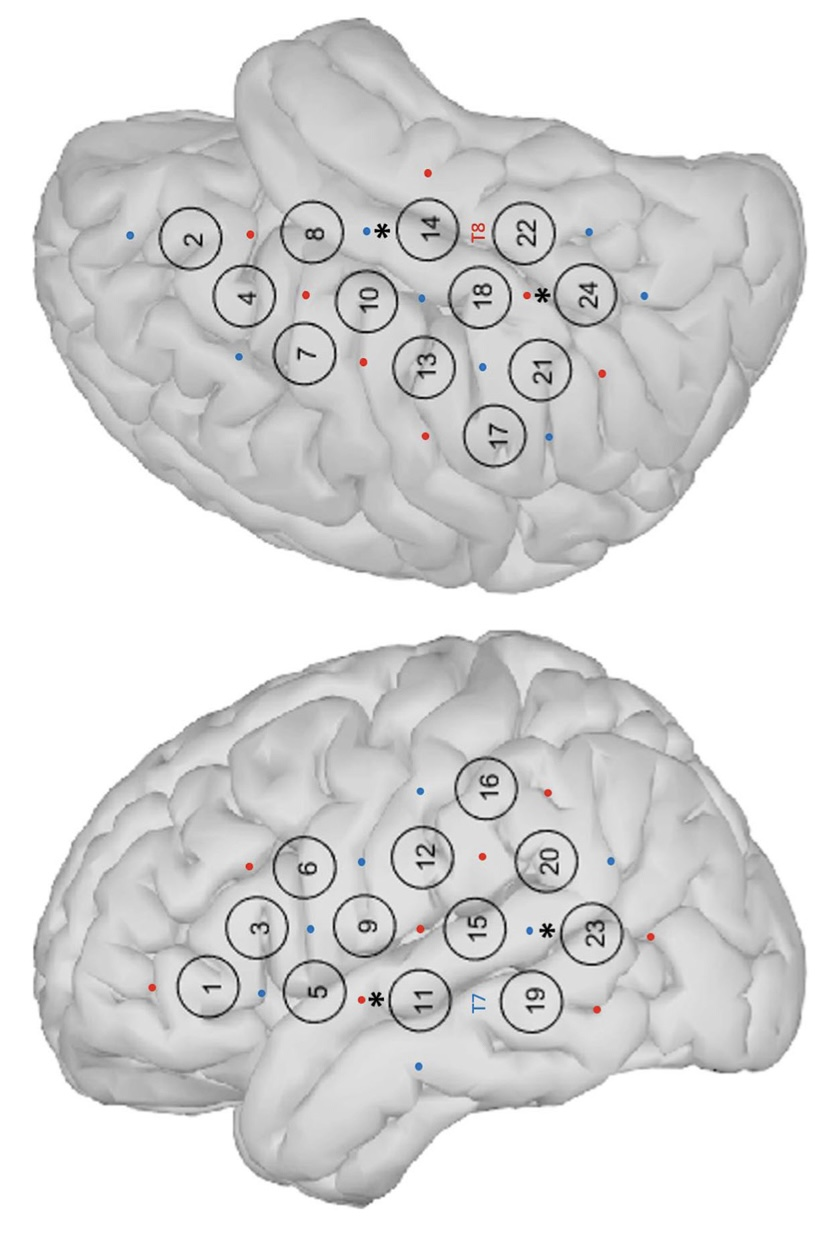
\includegraphics[scale=.5]{bilder/weder_probe.jpg}
  \caption{Probe design from Weder et al.}
  \label{fig:somesignal}
\end{figure}

Due to device limitations, we only measured one side of the brain. According to previous research \cite {Frost1999-vs} , language processing has been predominantly associated to cortical activity in the left hemisphere. As a result, we've decided to focus on the left hemisphere.

The fNIRS device we use also has limited number of sources and detectors. If we'd like to keep the original design, we'd need 9 sources and 9 detectors. However, the device we are using has only 10 sources and 8 detectors. Hence, we shifted one channel around T7 a little bit to the left, so that one less detector is needed. At the end, there were 12 long channels and 2 short channels in out setup.

For the software usage, an .xml file is required . In the .xml file, the sources, detectors, and channels are defined. Different optode templates for different probe design can be stored in one single .xml file. The physical cap was self-made from a swimming cap. With the help of a dummy head model, correct positions of the optodes were marked and holes were drilled accordingly. The mounts were put on the cap on the holes. In order to ensure the correct channels length to be fixed exactly at 30 mm, plastic holders were also placed on the long channels. As for the short channels, the  package comes with mounts for short channels. Thus, no plastic holders were needed in the case. The short channels were 11 mm long. The self-made cap turned out to work out well. The contacts between the scalp and the optodes were good thanks to the elastic characteristic of the material.

\section {Acoustic Stimulation during fNIRS Experiment}
Auditory stimuli were delivered binaurally via an audio metric headphone (Sennheiser HD 650). Stimuli consisted of 20-s chunks of the ICRA noise \cite {Dreschler}. 

To begin with, ICRA noise was developed to be used as background noise in clinical tests of hearing aids and possibly for measruing characteristics of non-linear instruments. The signals are based on live English speech from the EUROM database \cite {chanEUROM} in which a female speaker is explaining about the system of arithmetical notation. The speech signals were sampled with a sampling rate of 44.1 kHz. By composing the speech signals with well defined spectral and temporal characteristic, the modified signals have long-term spectrums but are completely unintelligible. 
 
We chose to use ICRA noise as stimuli based on several reasons. For one, ICRA noise is broadband amplitude-modulated signal. By selecting a broadband stimulus, broad cortical auditory areas and be activated more strongly compared with simple static stimulus. The bandwidth of auditory stimuli is positively correlated with the mean percentage signal change and spread of cortical activation \cite {Hall}. Previous fMRI study also manifested that more complex auditory stimuli elicit greater response in most parts of the auditory cortes \cite {Belin}. For the other, ICRA noise is a well-known and accessible stimulus. It is also considered as an international de facto standard for hearing research. In this way, our results can be comparable with other researches.
 
As for choosing different sound level pressure, we picked 40 dB, 65 dB, 90 dB, and silent stimulus, i.e. 0 dB. Calibrations were performed using an oscilloscope, a G.R.A.S. Power Module Type 12AK,  and an artificial ear (G.R.A.S. 43AA). The artificial ear transform the SPLs (sound pressure levels) into electrical signals, i.e. voltages that can be measured by the oscilloscope. According to the instruction manual of the G.R.A.S. artificial ear, the measured level is 11.19 $[ \frac {mV}{Pa}]$ and we know the SPL in dB is defined as 
\[
SPL [dB] = 20 \cdot log \frac{P}{P_0} \text{ , where $P_0$ is $20 \mu$Pa}
\] 
Hence, the relation between SPL and measured voltage should be.
\[
V = 20{ \mu Pa} \cdot 10^{\frac {SPL}{20}}  \cdot 10^{\frac{Gain}{20}} \cdot 11.19 {\frac {mV}{Pa}} 
\]
The headphone with the artificial ear were setup together in the sound booth to ensure minimal environmental noise. The output voltages were measured with the oscilloscope. This way, the corresponding amplitude inputs for later MATLAB scripts for the desire SPLs can be determined.

MATLAB and Oxysoft were used during the measurement. In MATLAB, a chunk in the ICRA audio files was selected. It was multiplied with different amplitude levels for 4 SPLs and ramped by a 10-ms Hanning window. In each epoch, all four stimuli (0dB, 40 dB, 65 dB, and 90 dB) were played randomly once. After each stimulus, there was a 25-sec silence rest to wait for the hemodynamic response. For each participant, 8 epochs were conducted. The stimuli were marked with Labstreaminglayer to note which SPL it was. This Labstreaminglayer also acted as an interface between MATLAB and Oxysoft, so that Oxysoft could mark the time for each stimulus in the measurement data correctly in real time.

\section {fNIRS Setup}
The Brite23 was used in this research. It is light weight, has 10 sources and 8 detectors and can support up to 23 channels. The Brite23 fNIRS device was connected via bluetooth to the PC and the Oxysoft software. For each measurement, the DPF is calculated depends on the age of the participant. The sampling rate was fixed at 50 Hz, for enough resolution but not unnecessary too large in terms of data size.

After the setting in the Oxysoft software was done, the participant would be asked to put on the self-made cap. On each optode position, the hair would be put aside gently with a Q-tip to ensure better contact between the optodes and the scalp. Then, the participants would be asked to put on the headphone and go into the sound booth.


\section {Data preprocession}
Data preprocessing and analysis was executed in MATLAB (Mathworks, USA) and the Homer3 toolbox. The following steps were executed.

First, the hemodynamic response was extracted with the Homer3 toolbox. Raw data were converted into optical densities. Motion artifacts were removed by using wavelet transformation of the data. The Homer3 toolbox bandpass filter (0.01 and 0.5 Hz) reduced drift, broadband noise, heartbeat, and respiration artifacts. Concentration if oxygenated and deoxygenated hemogloblin were estimated by applying the modified Beer-Lambert Law. It is important that the noise due to motion artifacts, drift, broadband noise, heartbeat, and respiration artifacts need to be processed before the concentration was estimated, according to the previous research \cite {Huppert:09}.

Later on, the extracerrebral component in long channels should be reduced by using measurements from the short channels as follows: the first principal components from the two short channels were estimated and then multiplied by its coefficient from the GLM (general linear model).However, this is not done in the scope of this research. The coefficient from the GLM were very small. They were of the magnitudes $10^{-16}$ , whereas the hemodynamic response in the long channels were of the magnitudes $10^{-5}$. Hence, we concluded the extracerrebral components in our case can be negligible.

Channels with unusable data were excluded here for further analysis. The scalp coupling index (SCI) is a common measure in this case. It is originally described in \cite {polloniniSCI}. In short, the SCI estimates the correlation between the two wavelength channels in the cardiac band as the following:

First, the signal is bandpass-filtered to keep only the cardiac band. In our case, a wide band of [0.5 - 2.5] Hz was chosen. Then, amplitude normalization is performed, and the SCI computation is defined as the absolute cross-correlation value at 0-time lag.


\begin{figure}[H]
  \centering
    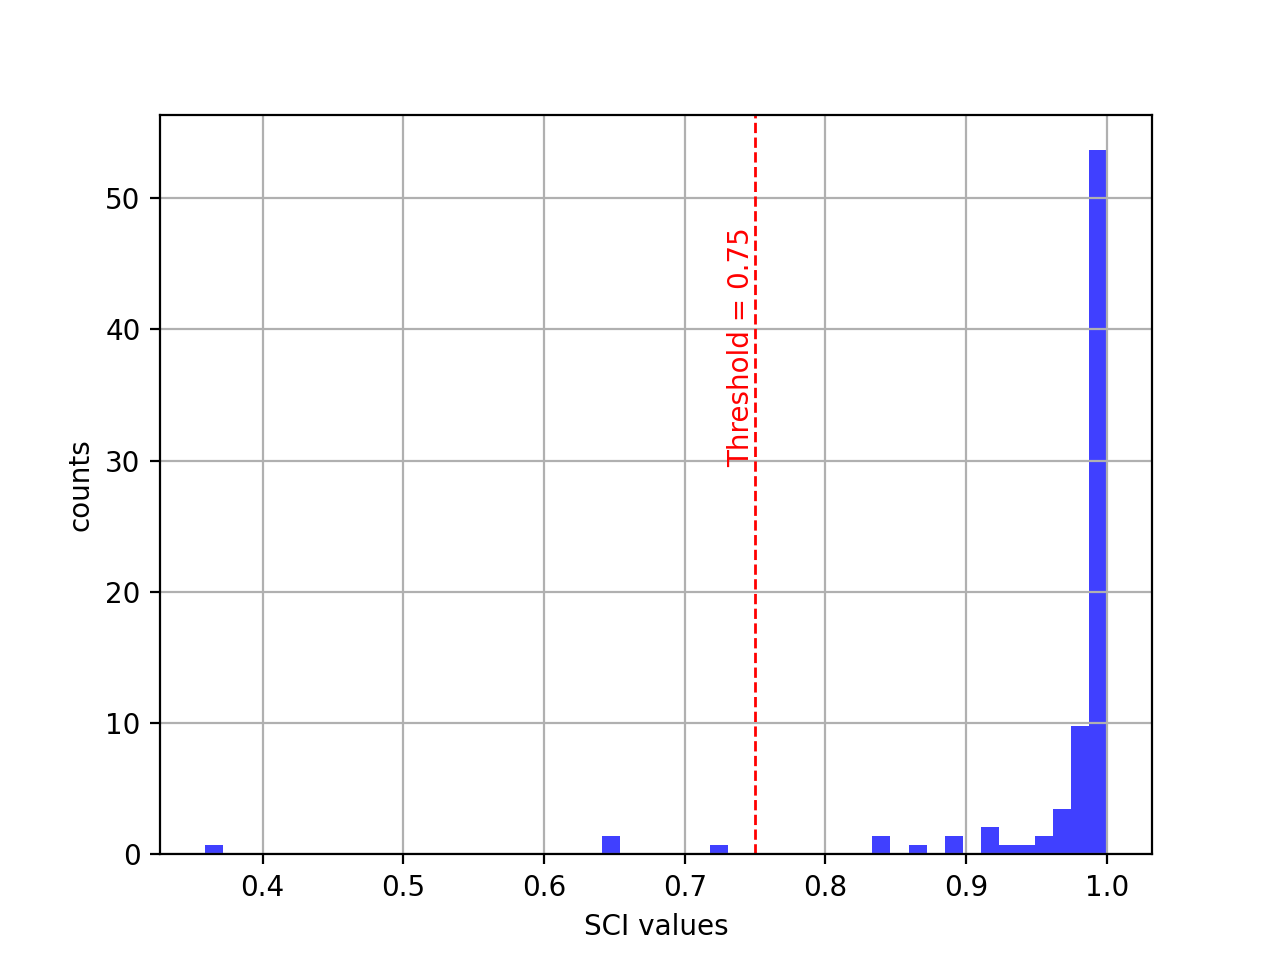
\includegraphics[scale=.75]{bilder/SCI_hist.png}
  \caption{Distribution of SCI values for all measurements. Threshold : 0.75}
  \label{fig:somesignal}
\end{figure}





\chapter{Results}
\section {Waveform Morphology}
From our measurements, the results varied a lot individually. Hence, grand average and further statistical analysis would not be well-applicable. In this section, waveform morphology of the 14-channel measurements for some of the participants are shown and described.

First of all, our channels with the optode template are defined as this figure.

\begin{figure}[H]
  \centering
    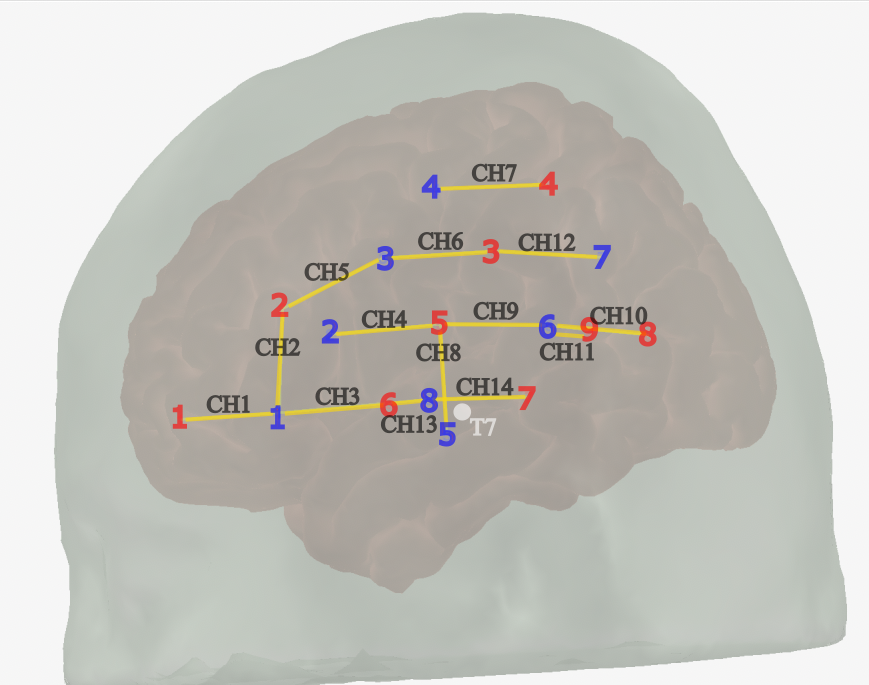
\includegraphics[scale=.45]{bilder/optode_ink.png}
  \caption{Channel Definition}
  \label{fig:somesignal}
\end{figure}

In the following figures. Channels with invalid SCI would not be taken into consideration, and hence would not be shown. Measurements in all channels were plotted in the same scale except for the two short channels marked in thicker outlines. In all our measurements, the changes in the dynamic hemoglobin response were significantly less in the short channels by more than a magnitude.

\subsection{Oxygenated Hemoglobin, HbO}
\begin{figure}[H]
  \centering
    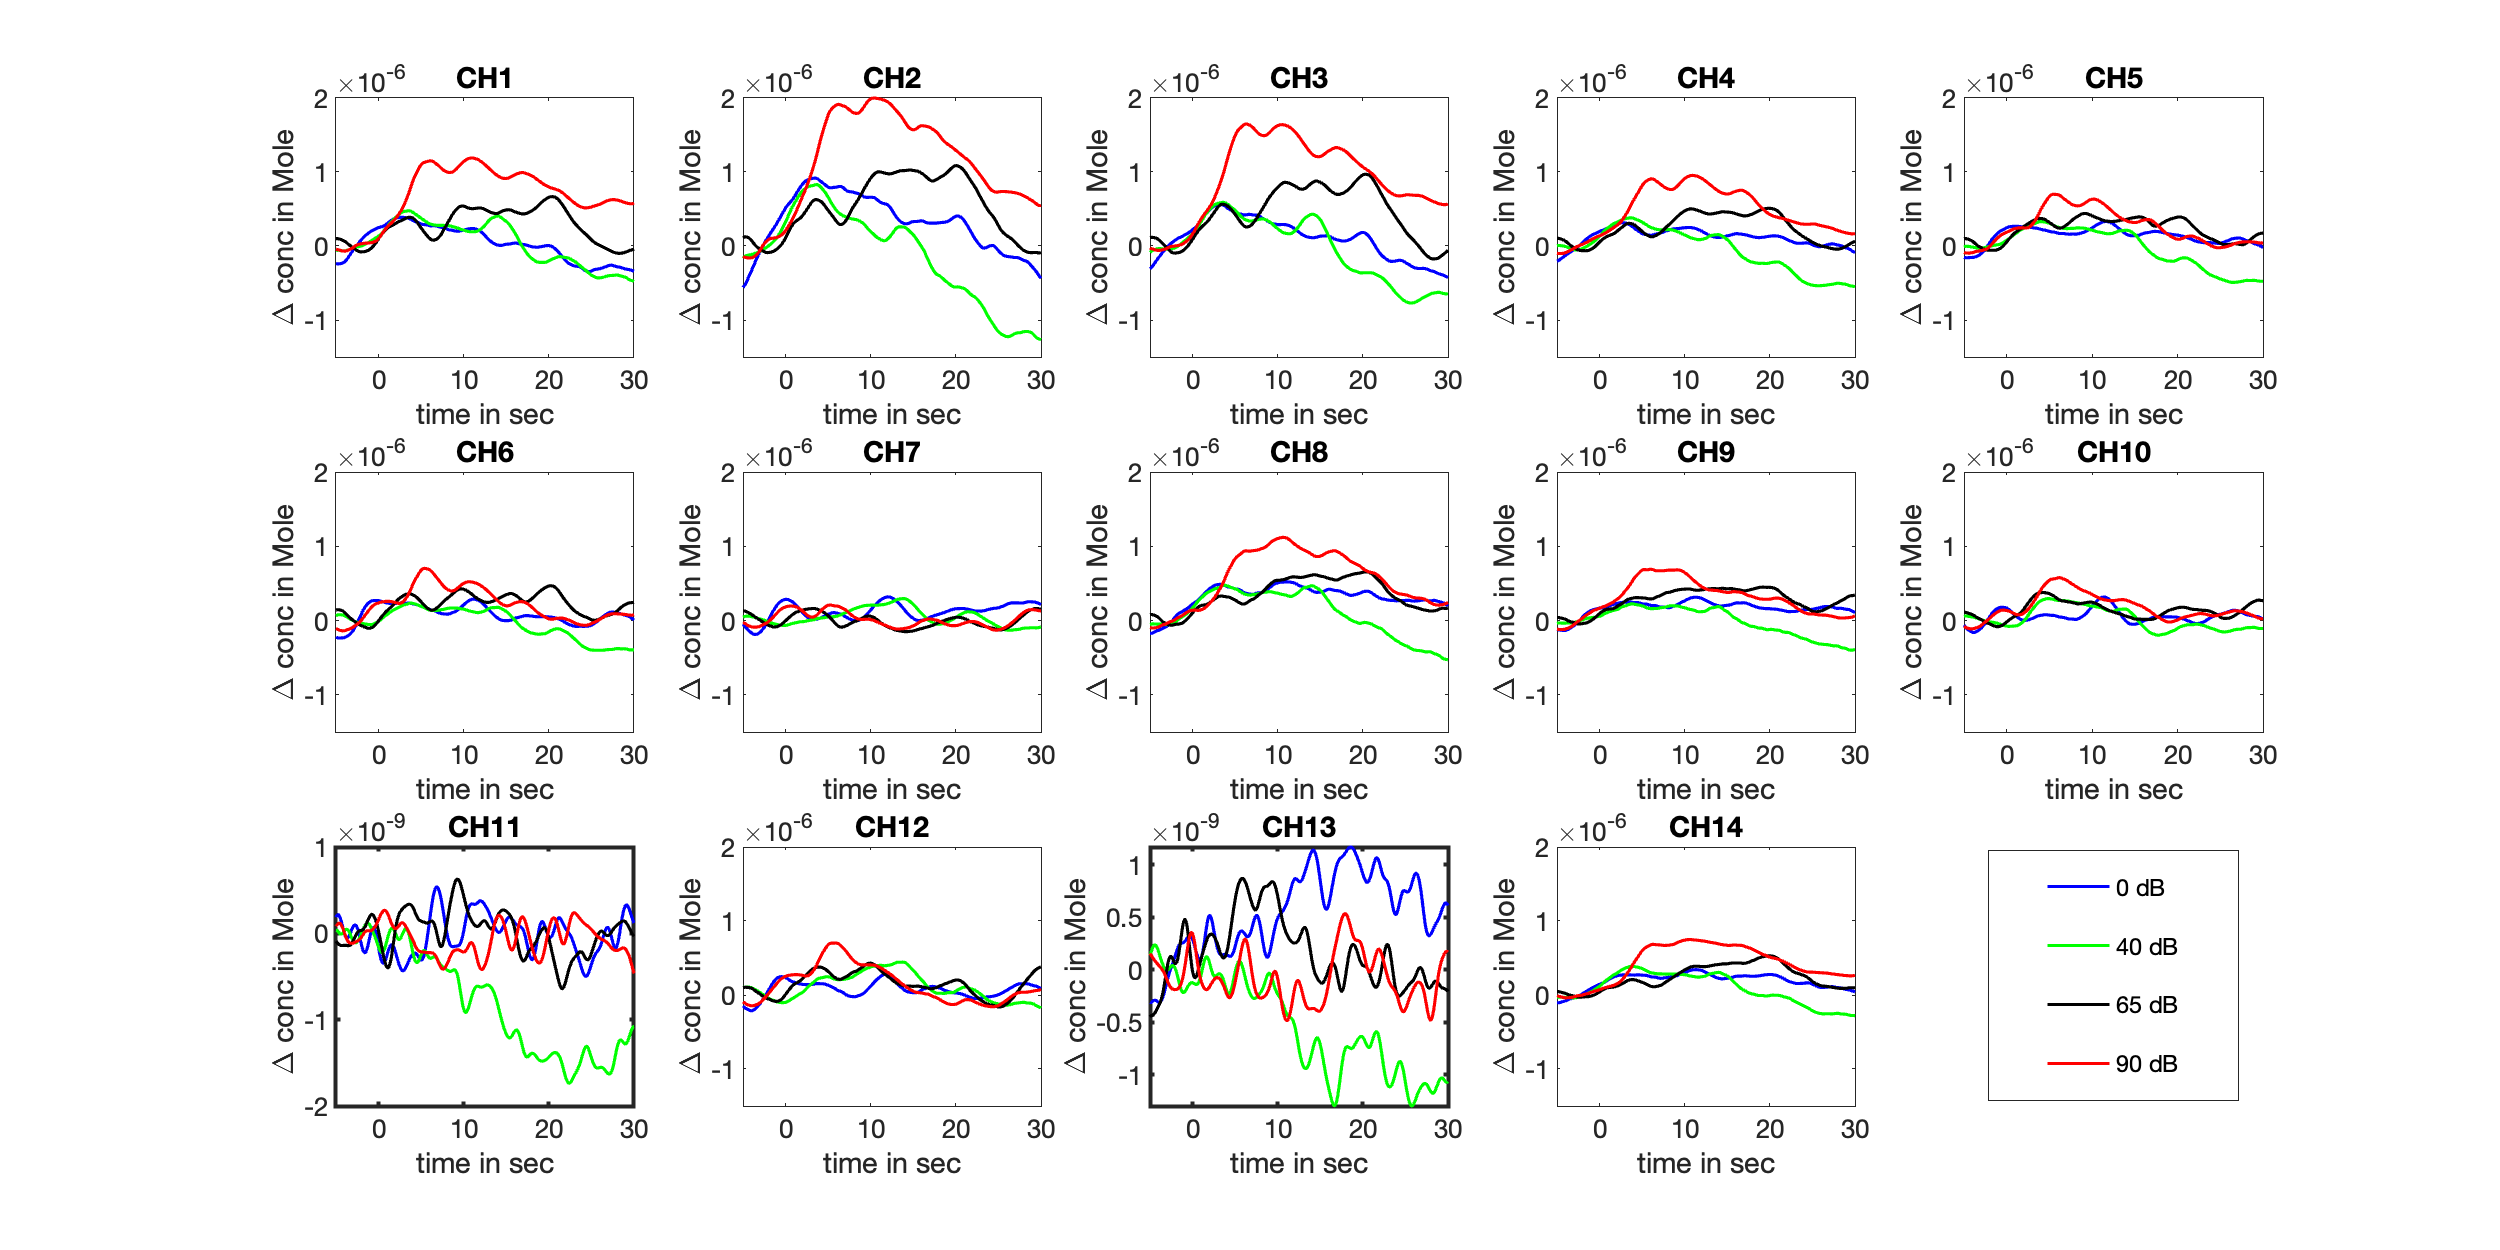
\includegraphics[scale=.4]{bilder/HbO_Mole/sub_jonas_s_HbO.png}
  \caption{Measurement from participant 3.}
  \label{fig:somesignal}
\end{figure}

\begin{figure}[H]
  \centering
    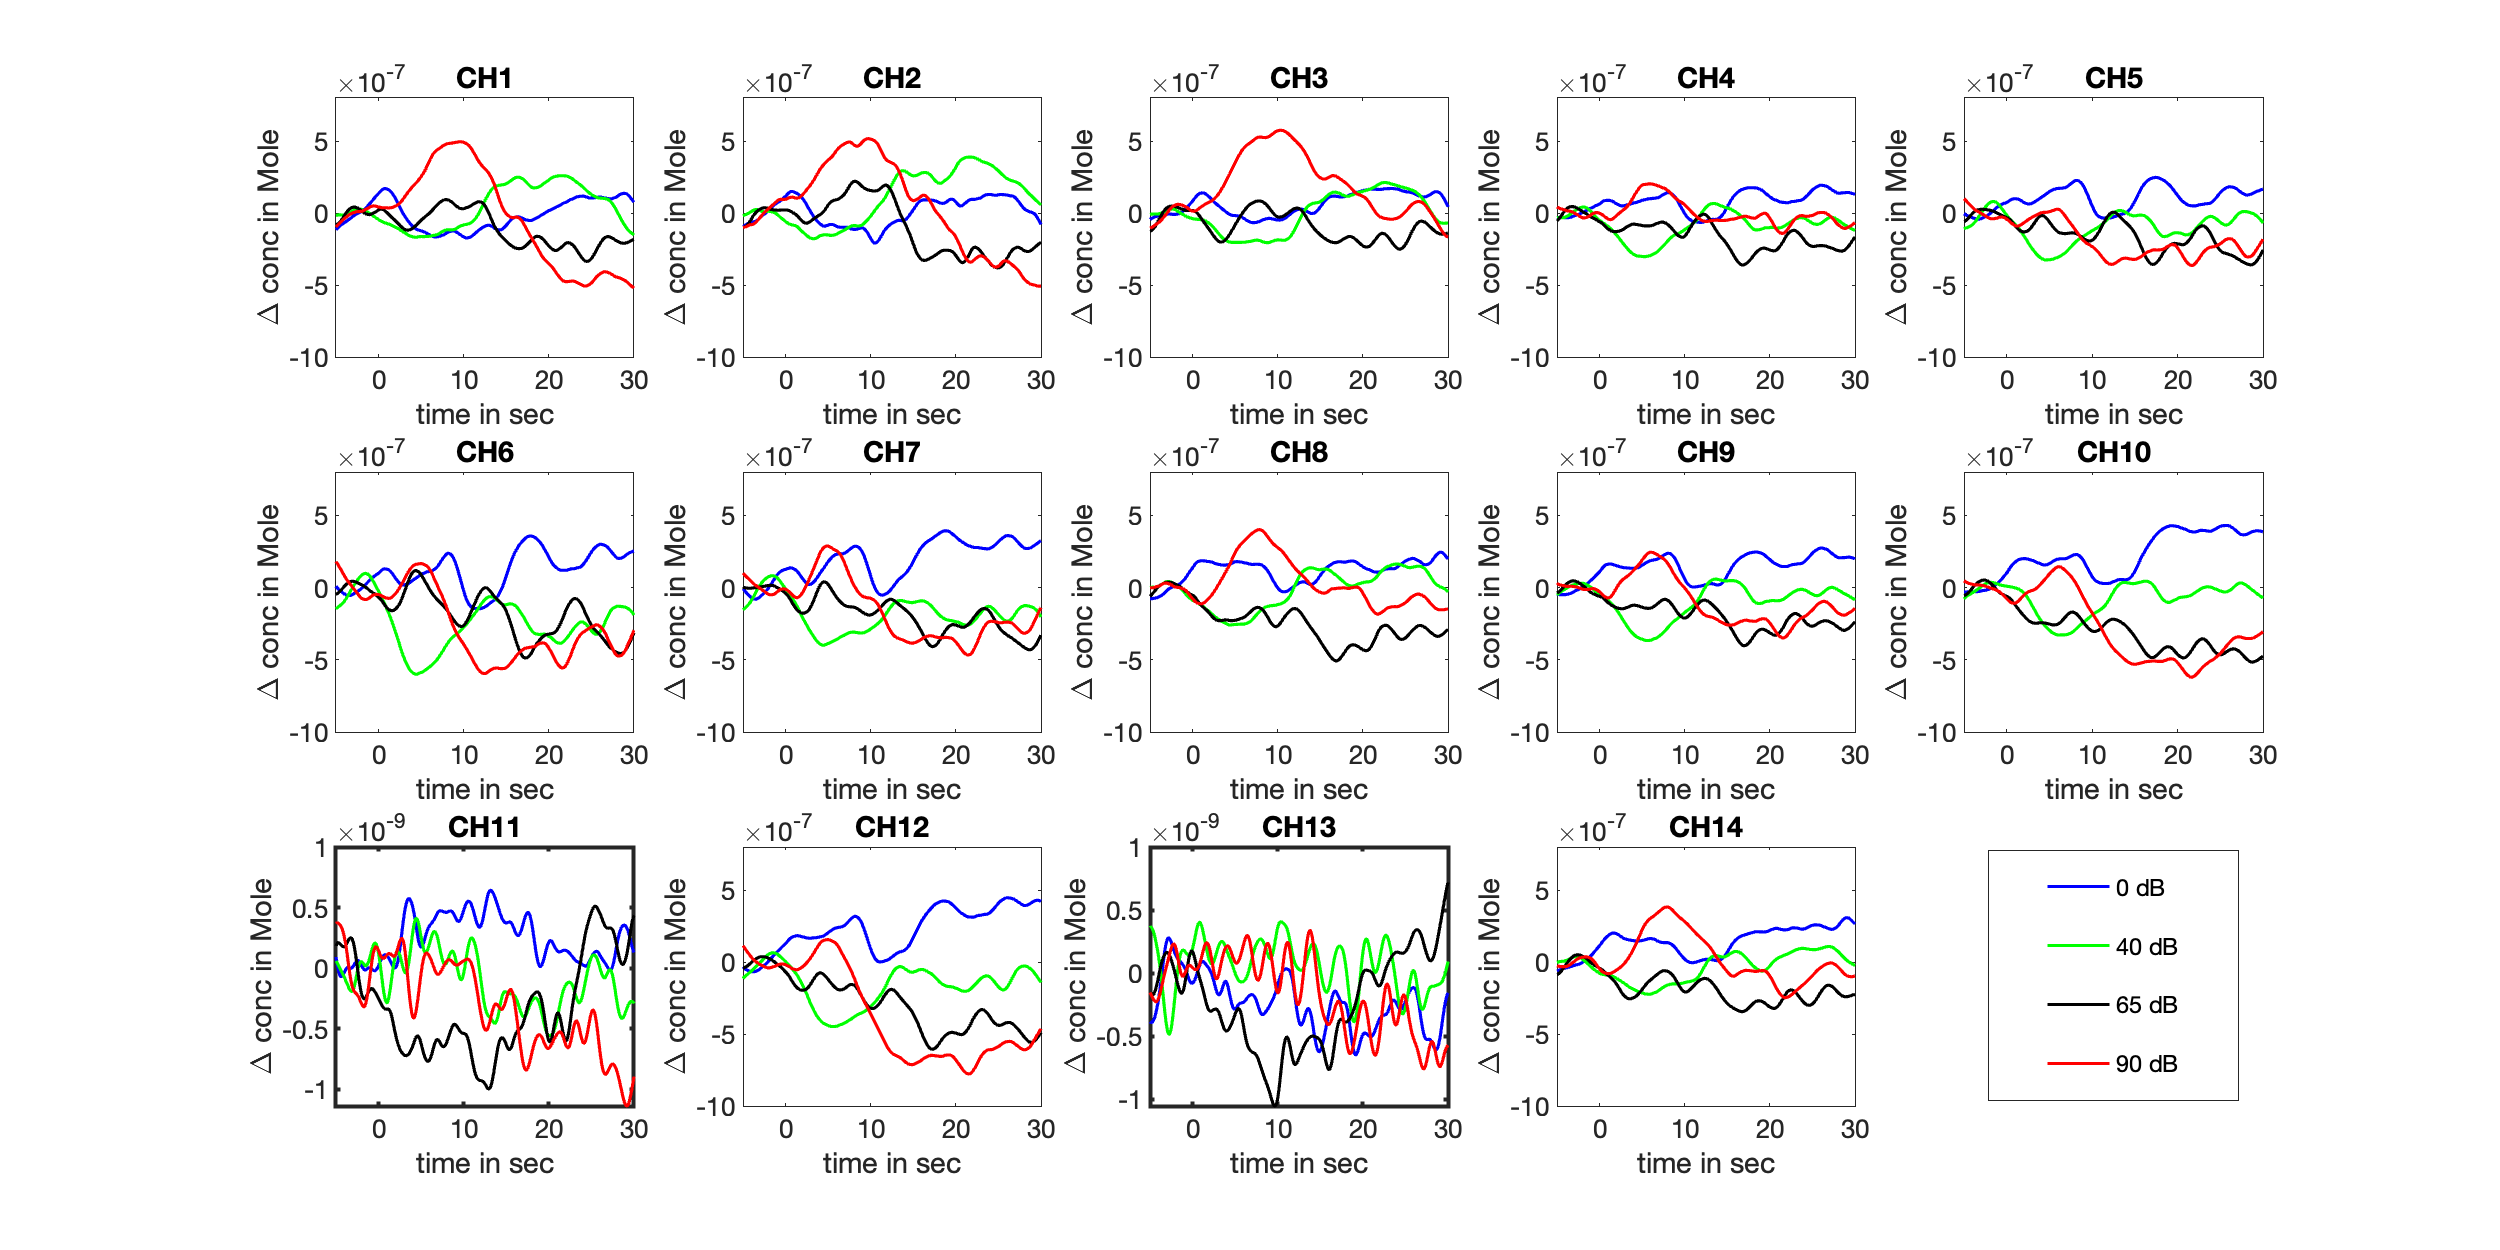
\includegraphics[scale=.4]{bilder/HbO_Mole/sub_lukas_s_HbO.png}
  \caption{Measurement from participant 5.}
  \label{fig:somesignal}
\end{figure}

\begin{figure}[H]
  \centering
    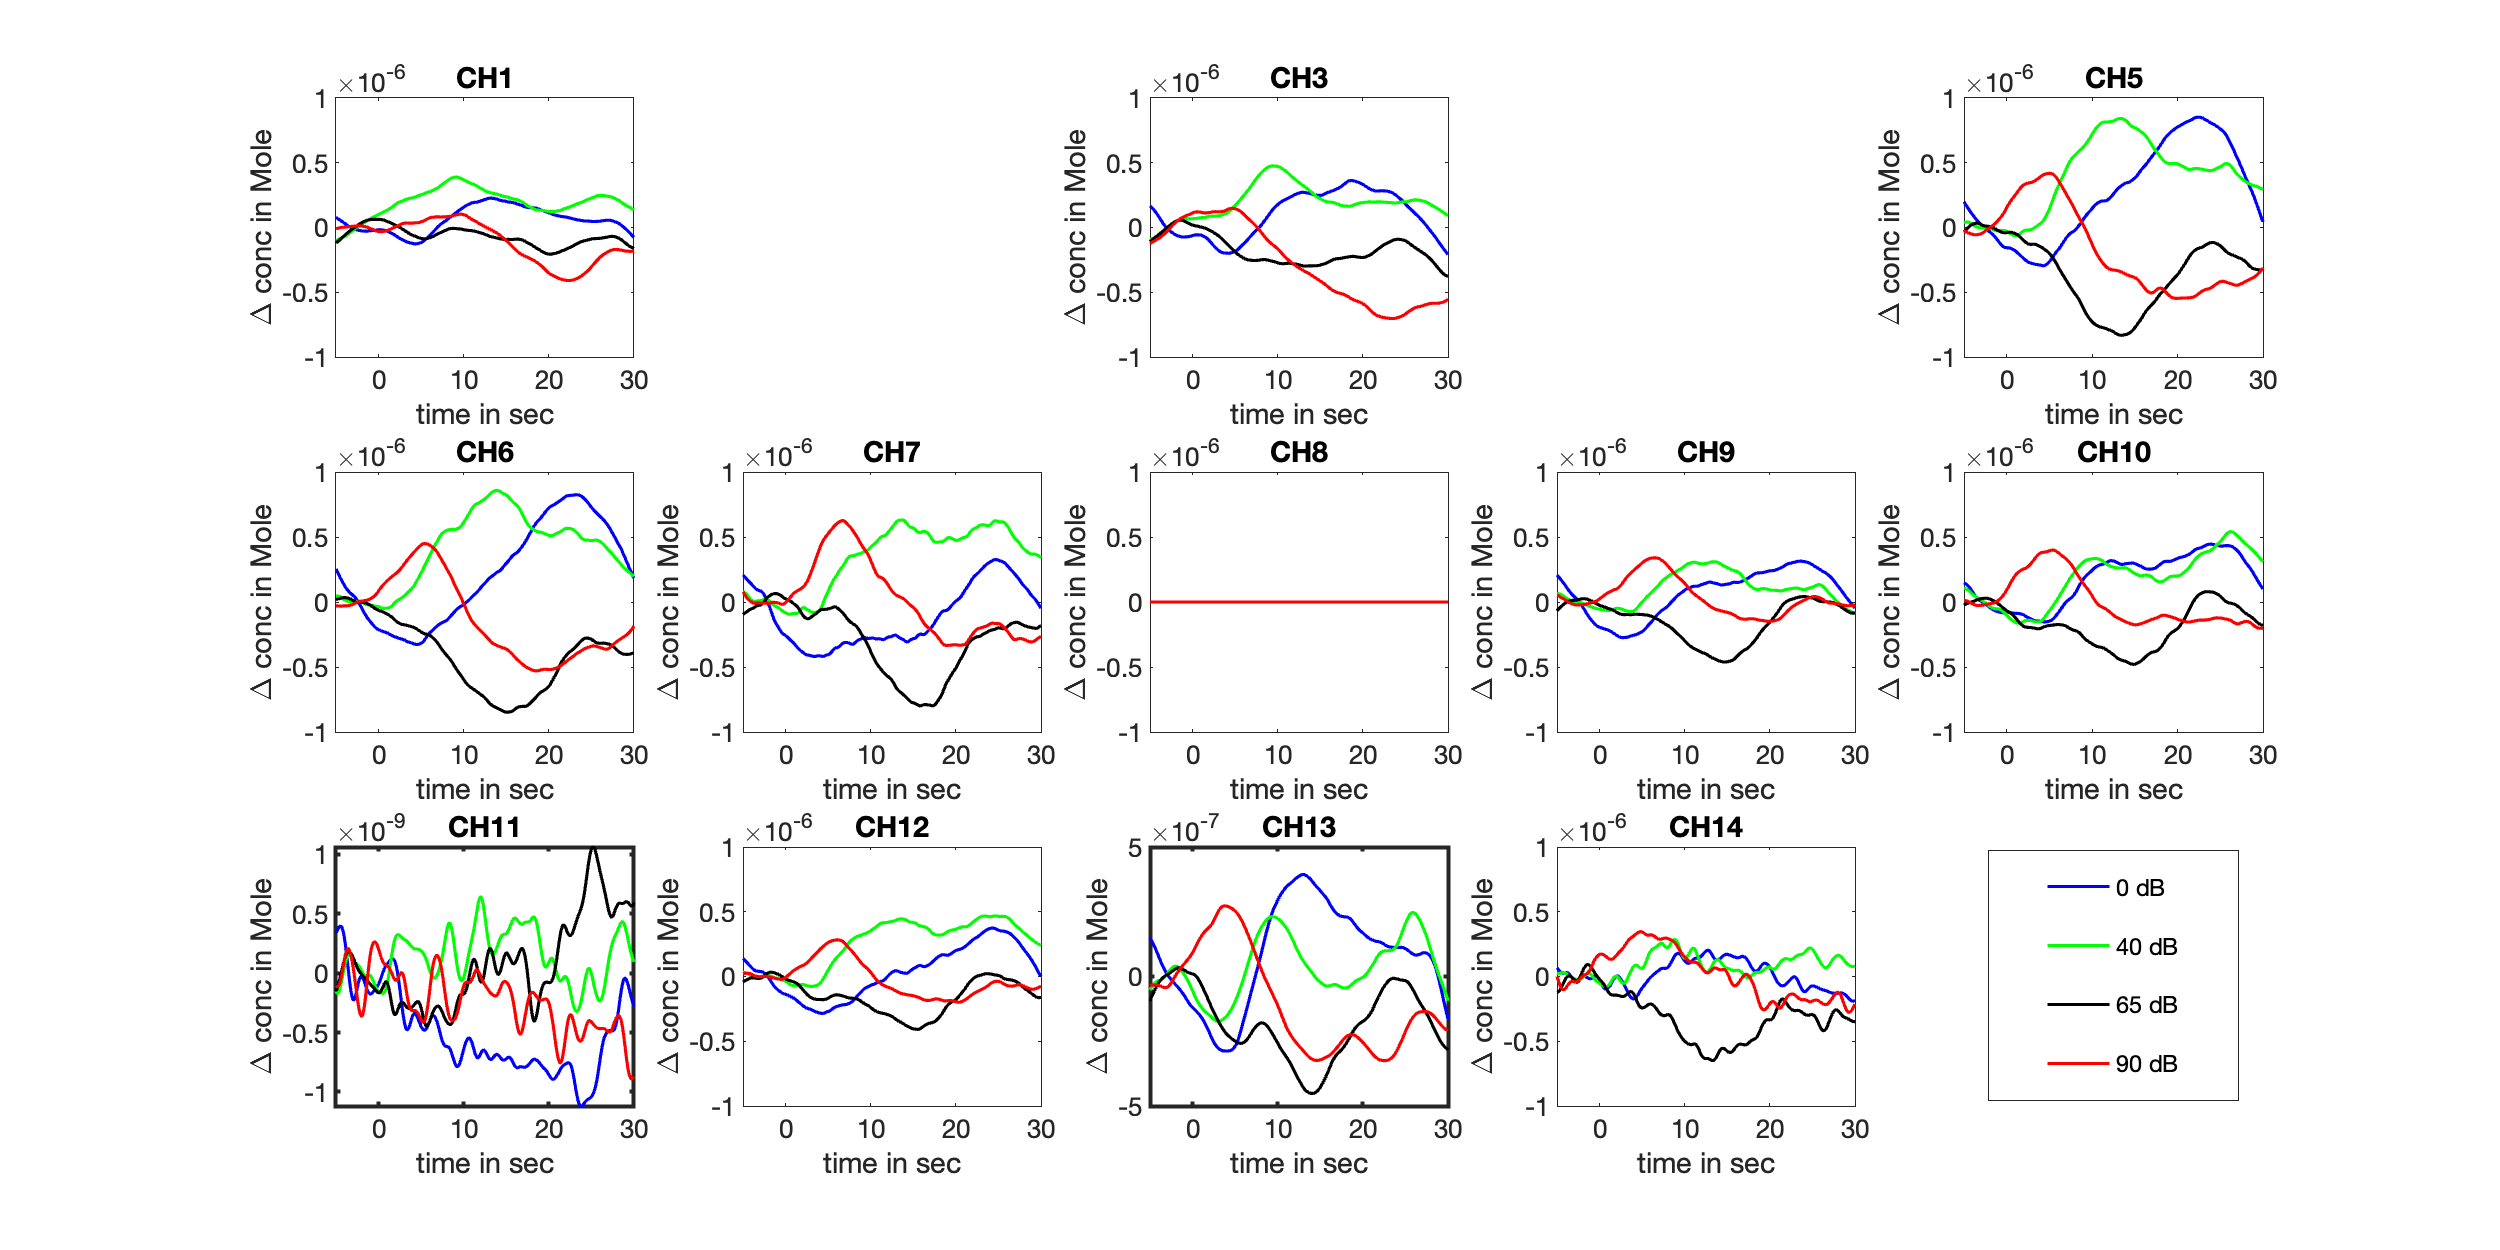
\includegraphics[scale=.4]{bilder/HbO_Mole/sub_shelia_s_HbO.png}
  \caption{Measurement from participant 6.}
  \label{fig:somesignal}
\end{figure}

\begin{figure}[H]
  \centering
    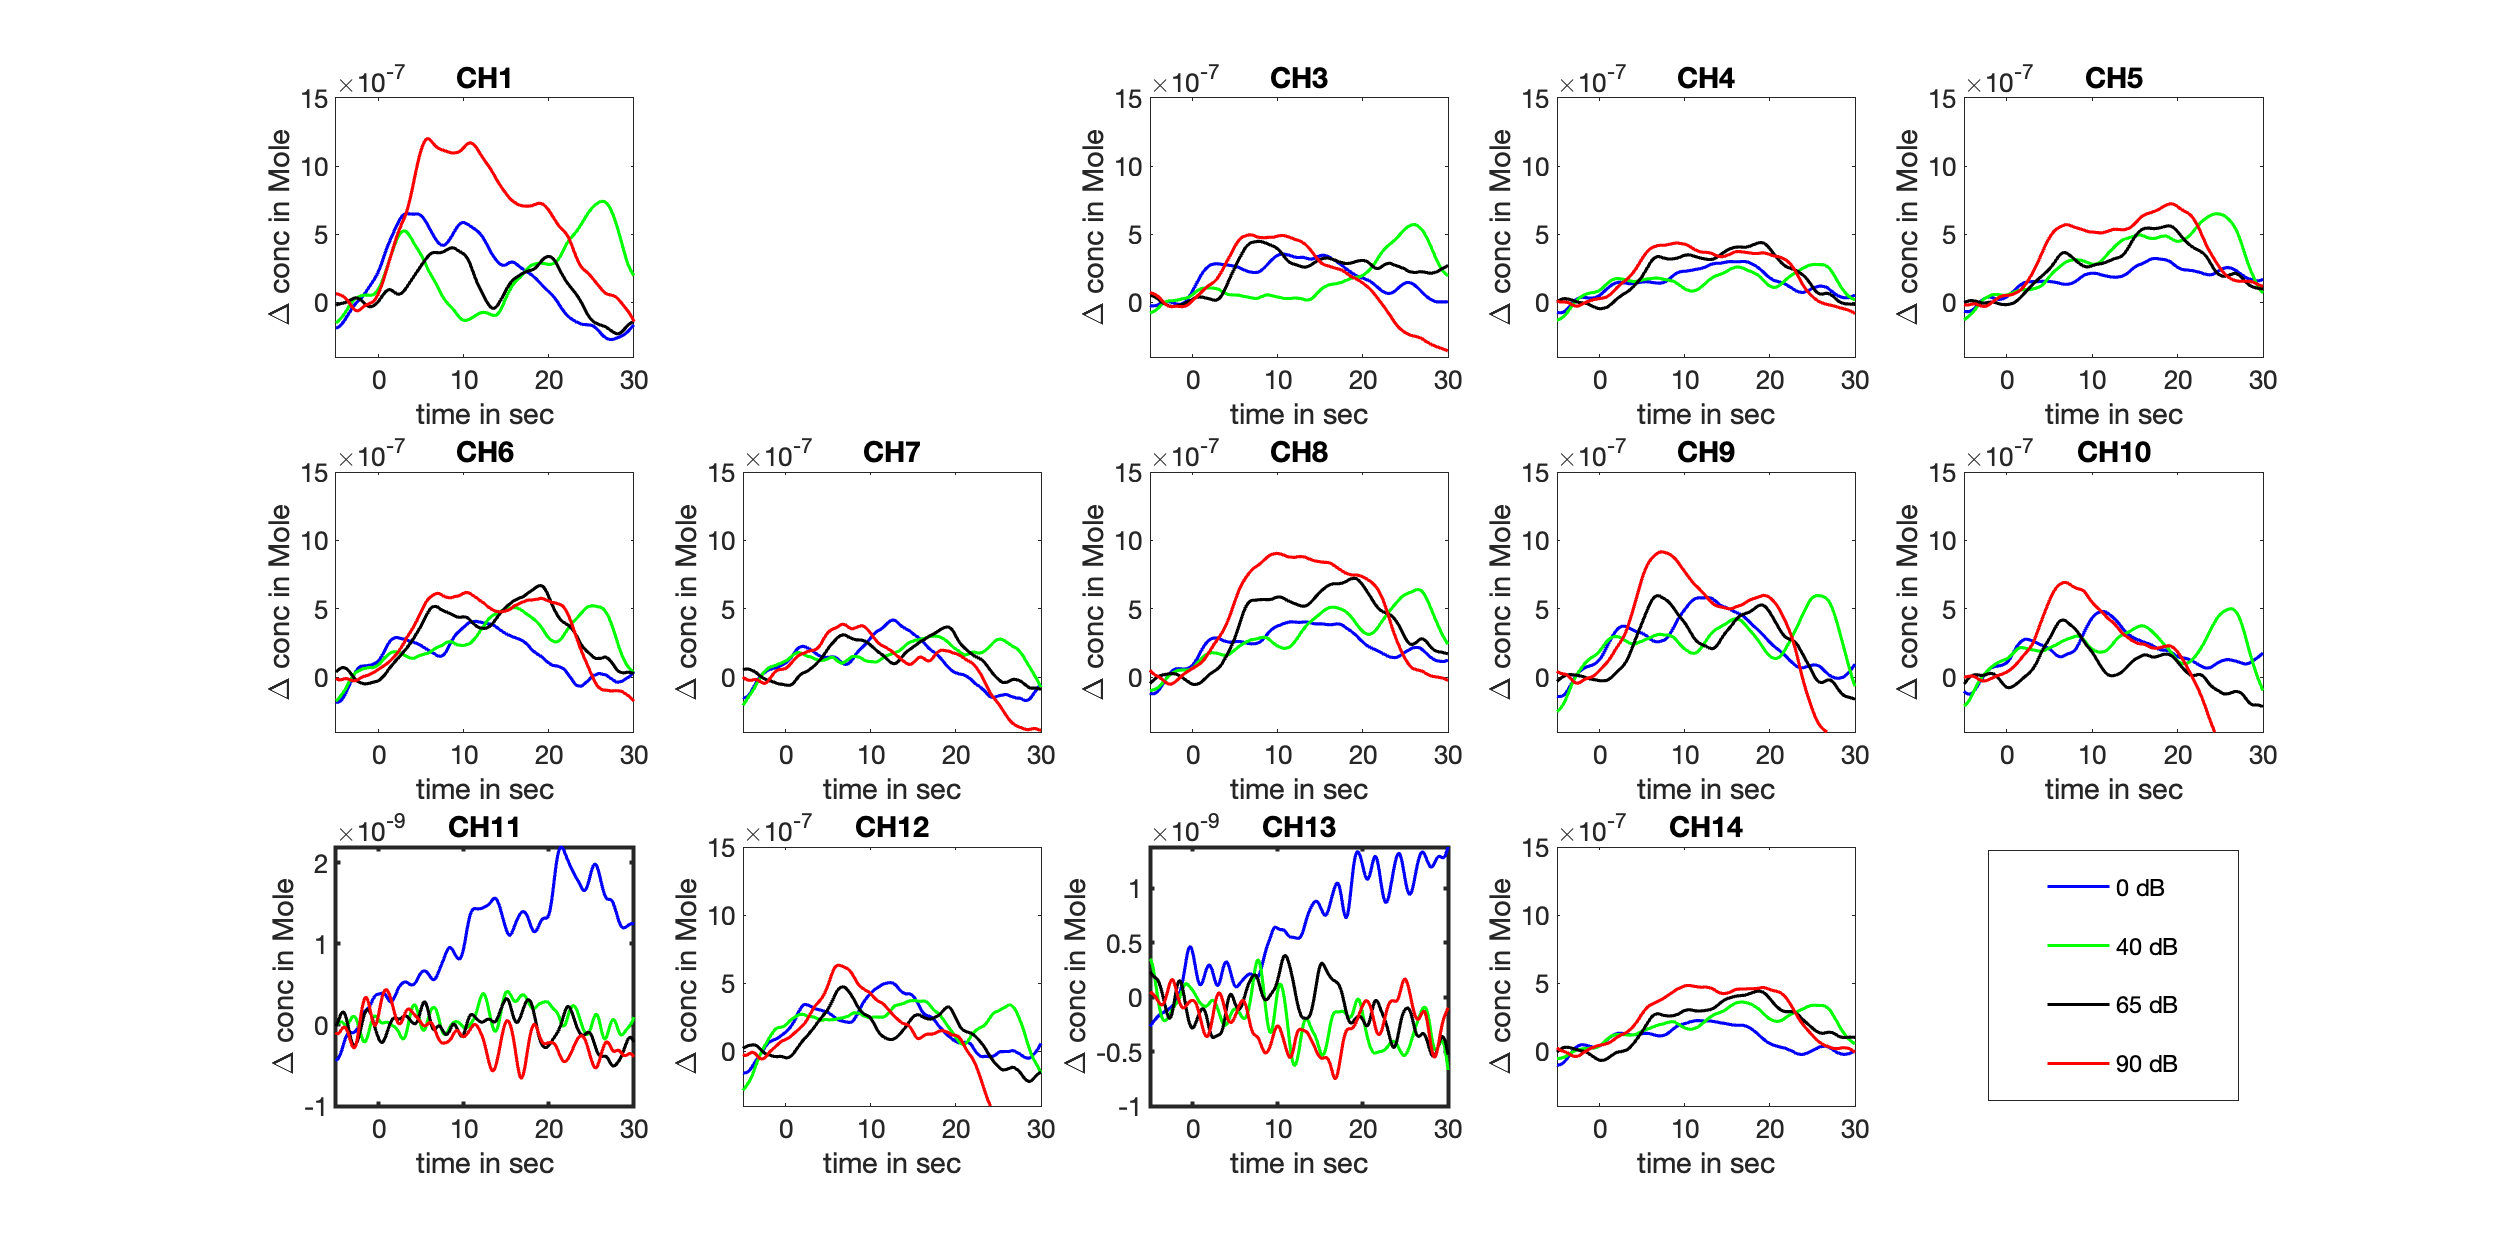
\includegraphics[scale=.4]{bilder/HbO_Mole/sub_liao_s_HbO.png}
  \caption{Measurement from participant 7.}
  \label{fig:somesignal}
\end{figure}


\begin{figure}[H]
  \centering
    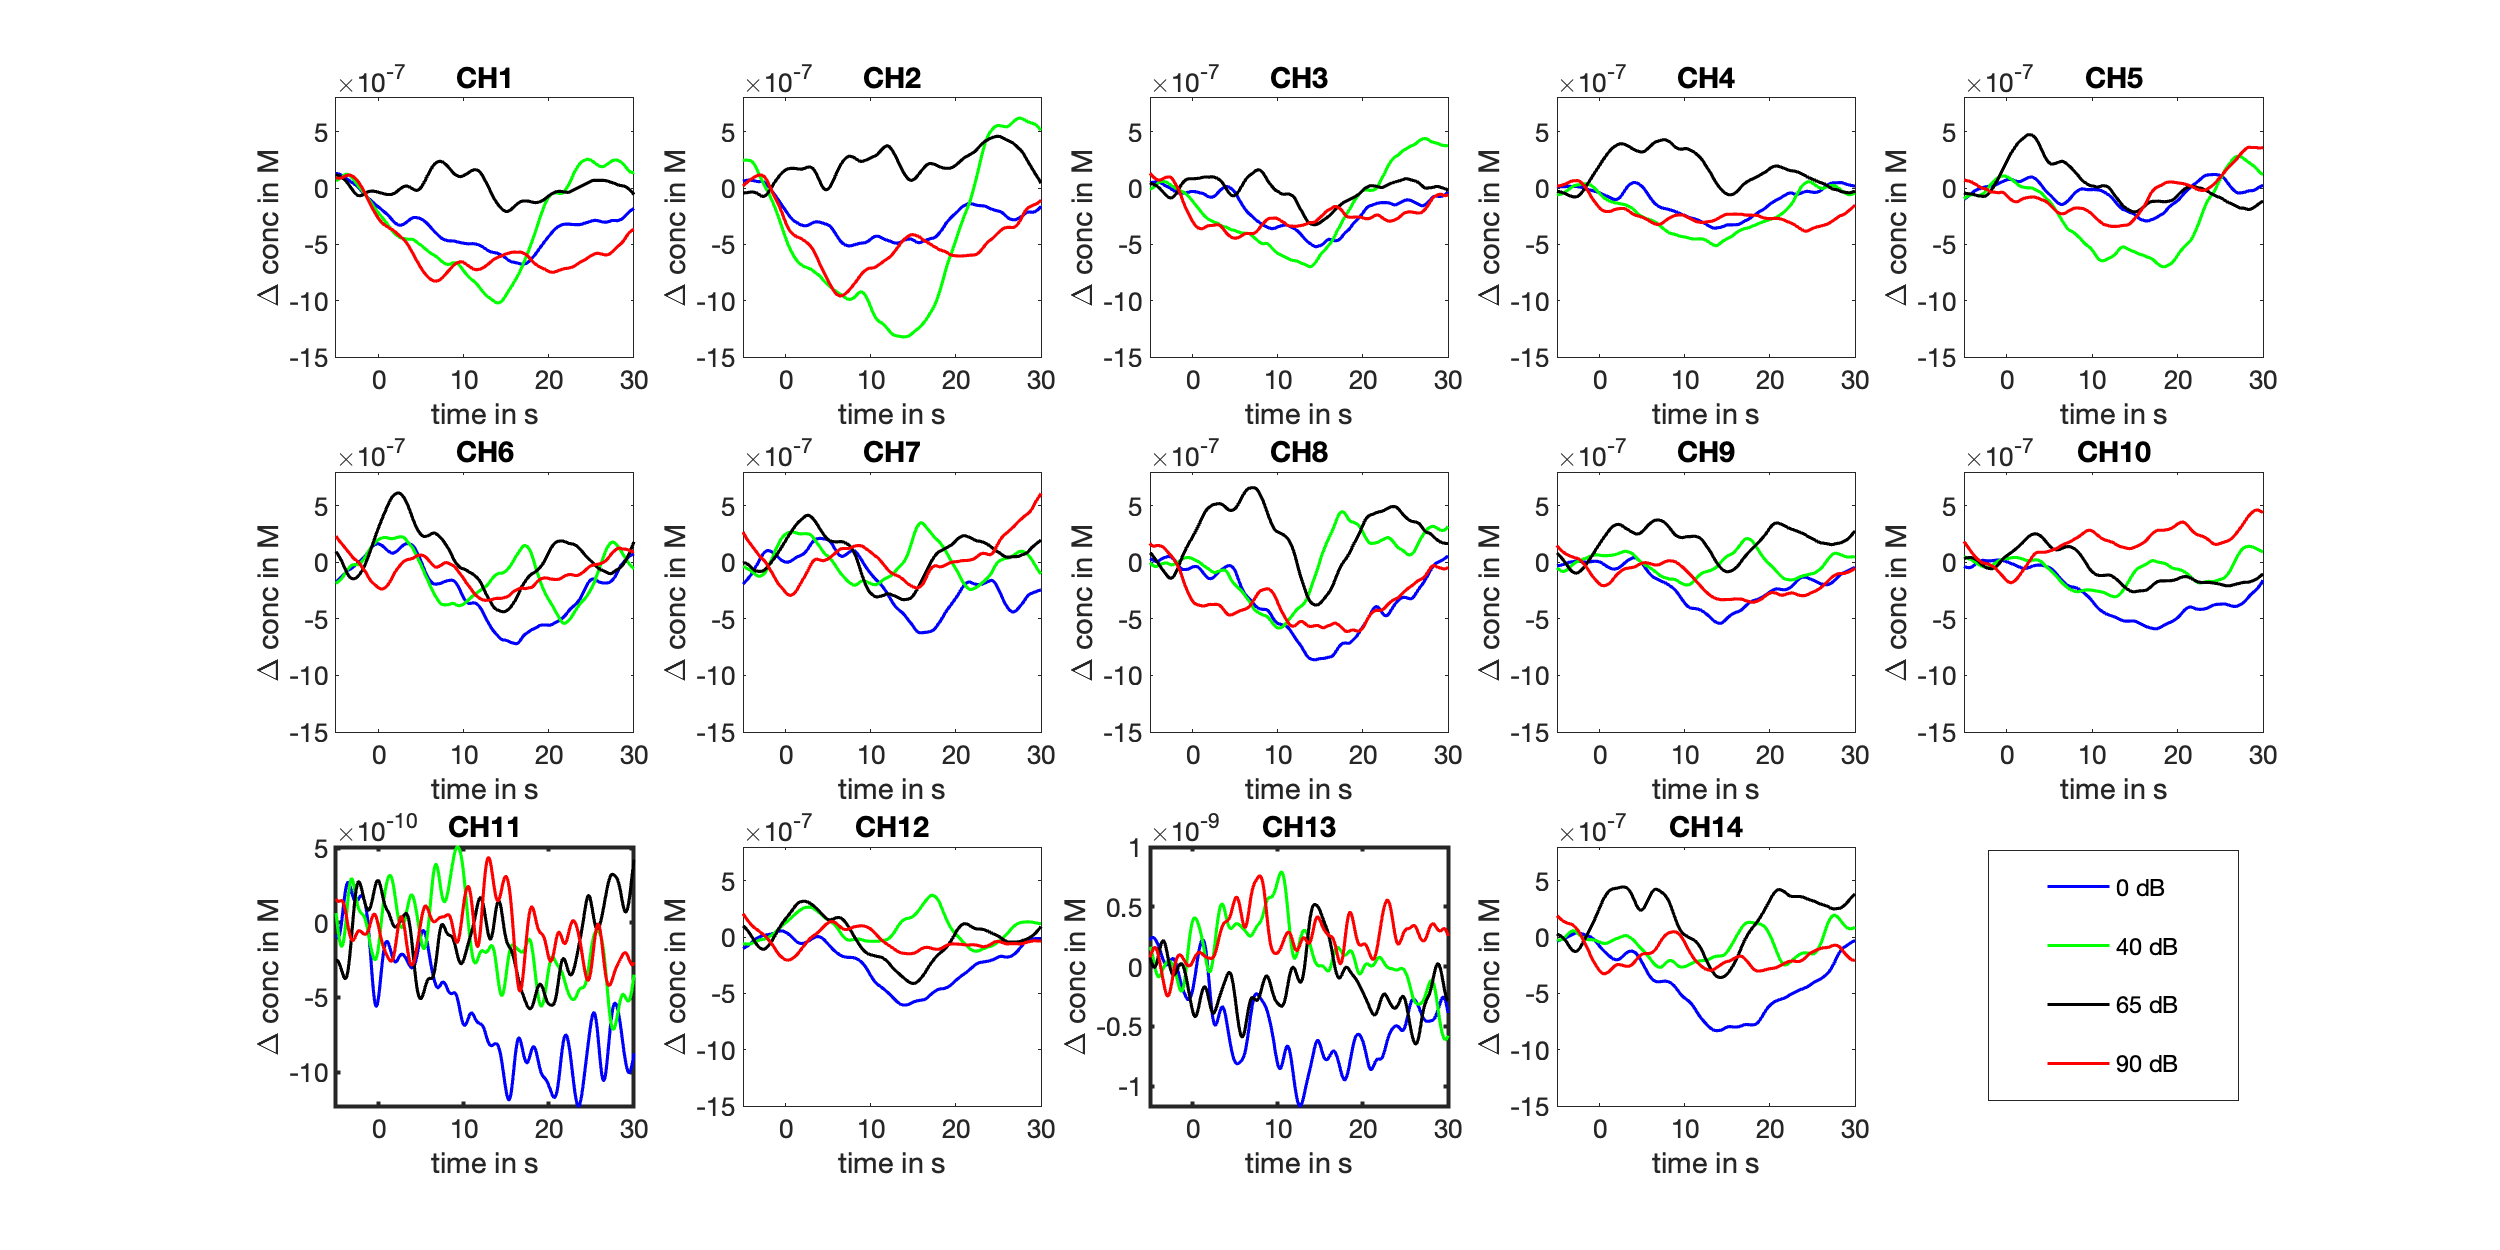
\includegraphics[scale=.4]{bilder/HbO_Mole/sub_luca2_s_HbO.png}
  \caption{Measurement from participant 8. Silent comparison}
  \label{fig:somesignal}
\end{figure}



\newpage

\subsection{Deoxygenated Hemoglobin, HbR}

\begin{figure}[H]
  \centering
    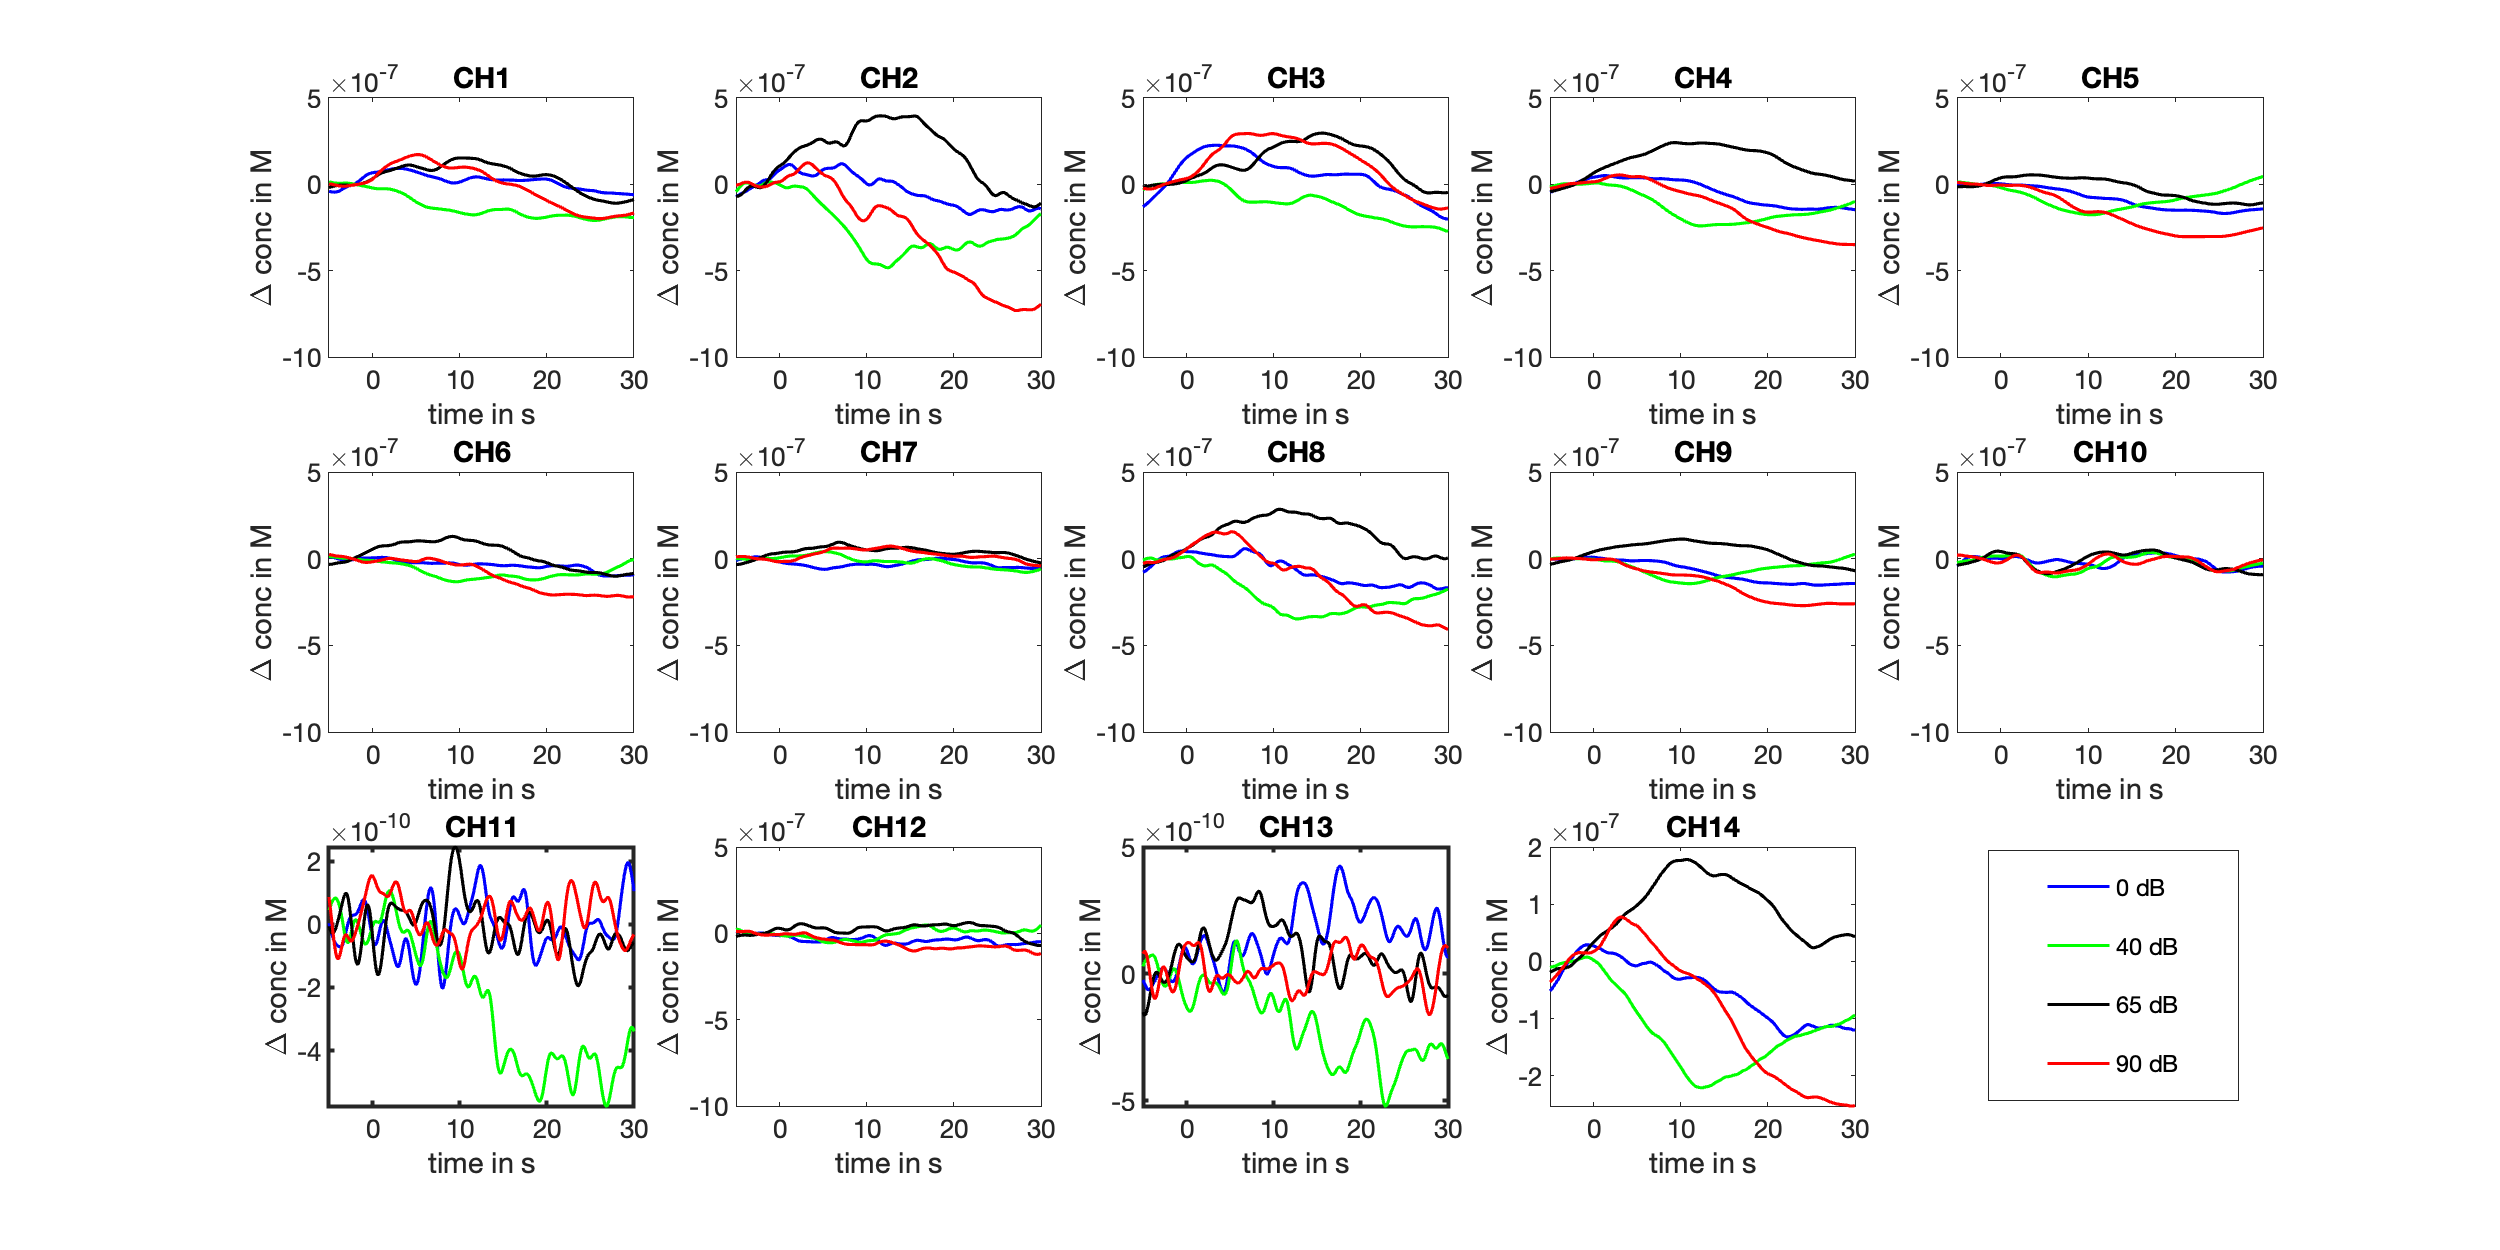
\includegraphics[scale=.4]{bilder/HbR_Mole/sub_jonas_s_HbR.png}
  \caption{Measurement from participant 3.}
  \label{fig:somesignal}
\end{figure}

\begin{figure}[H]
  \centering
    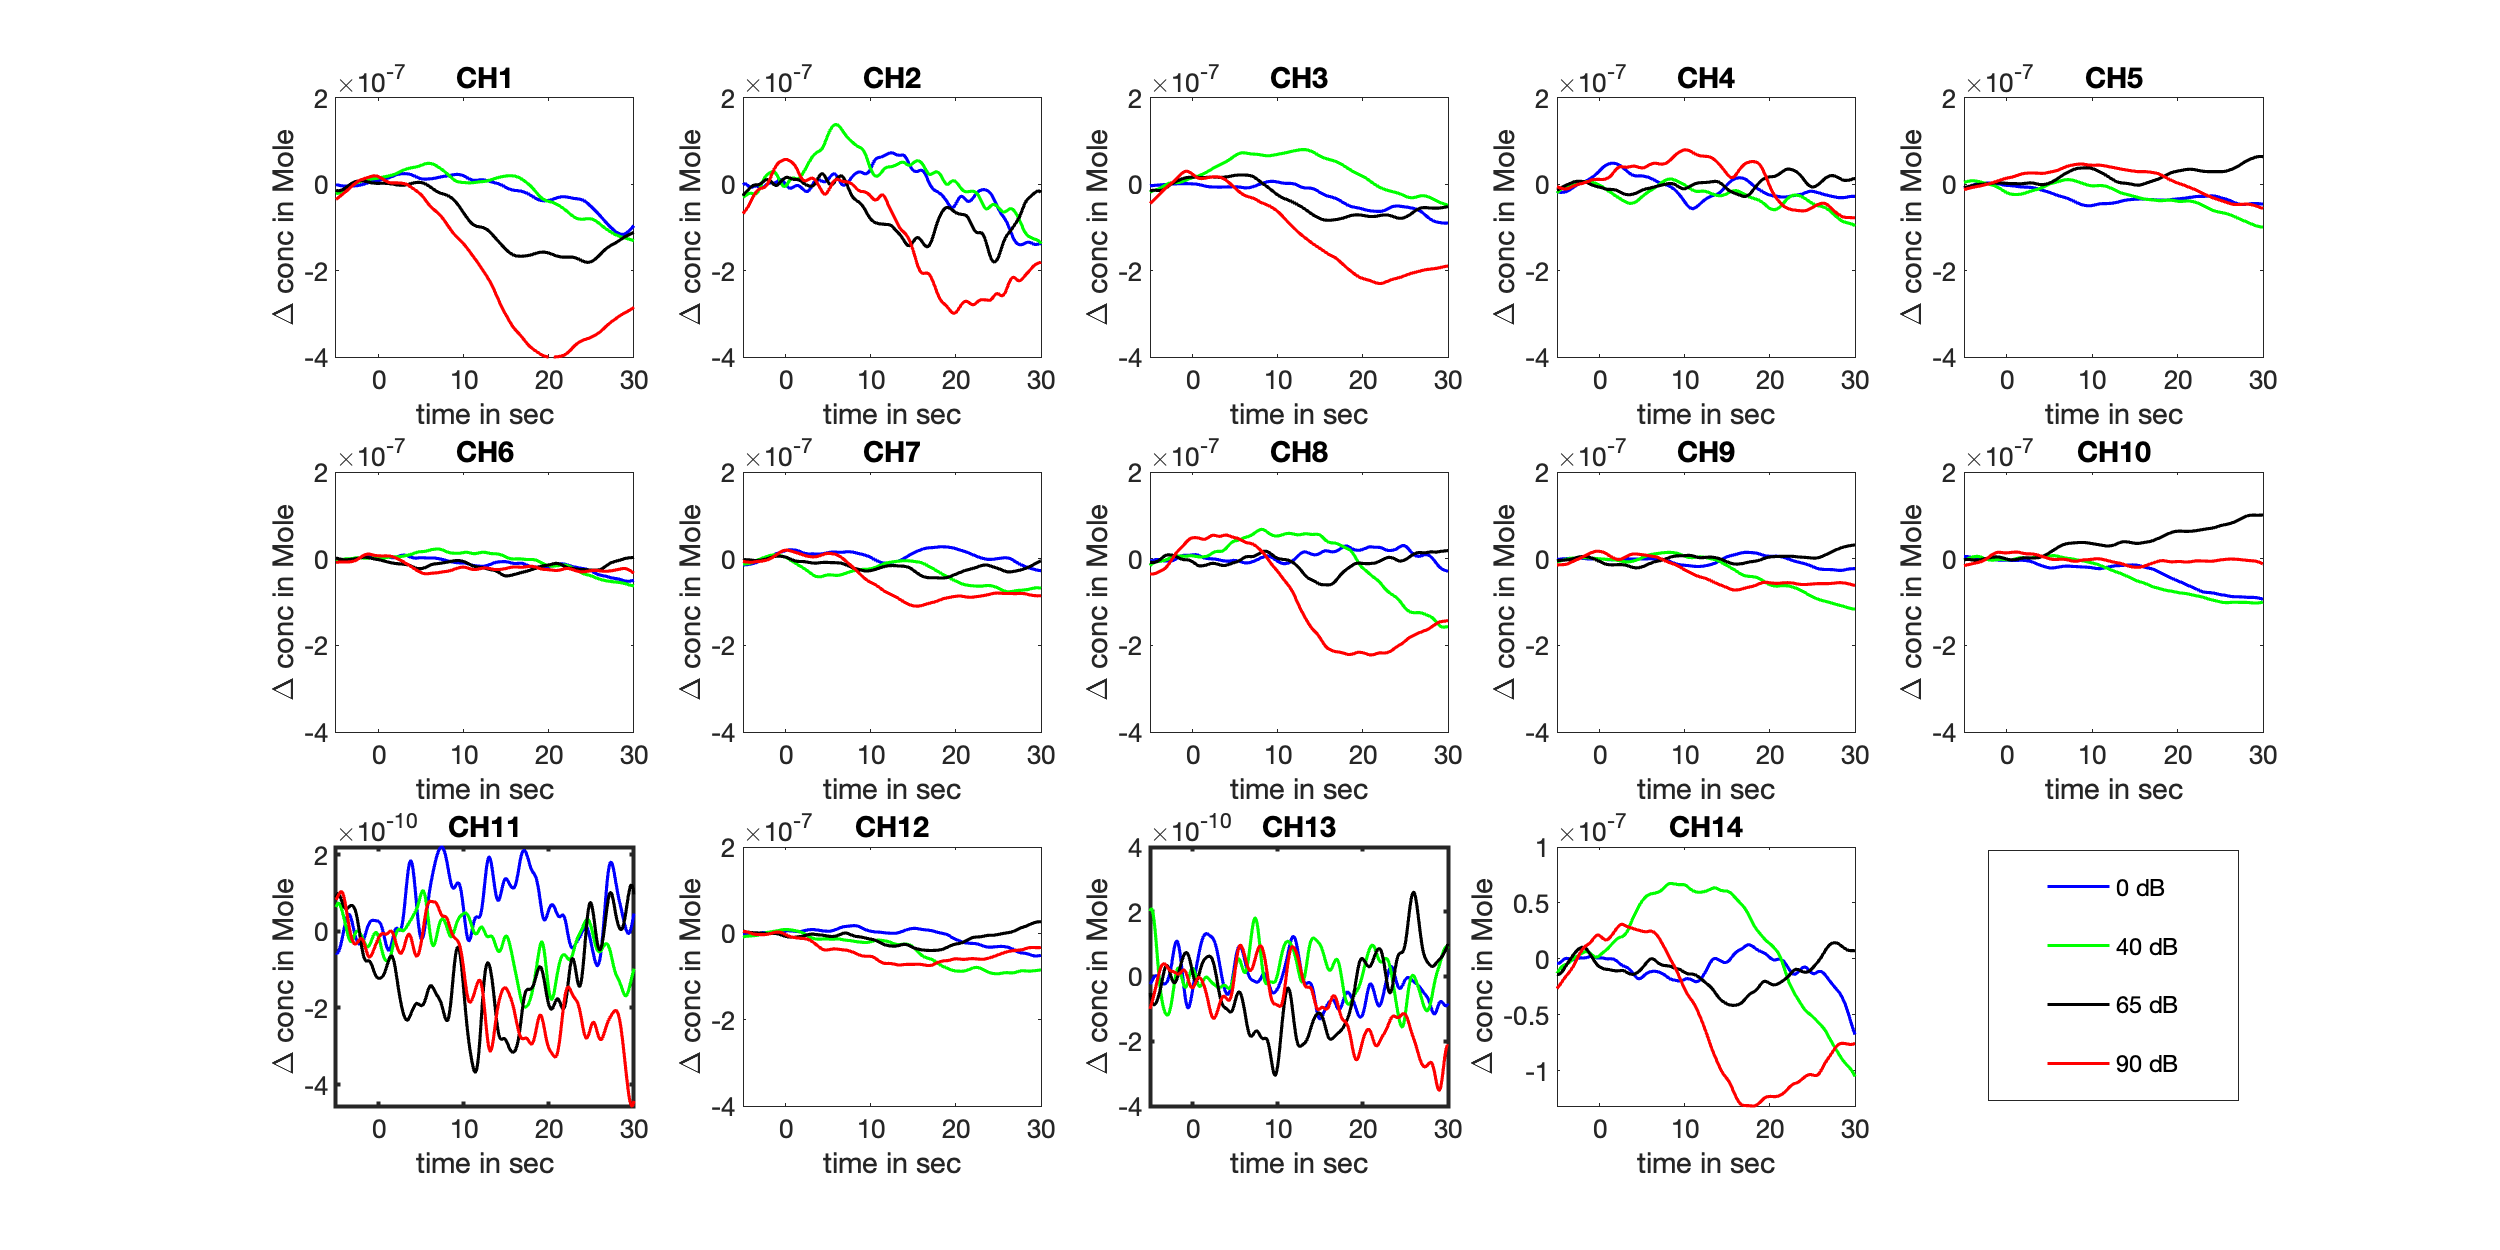
\includegraphics[scale=.4]{bilder/HbR_Mole/sub_lukas_s_HbR.png}
  \caption{Measurement from participant 5.}
  \label{fig:somesignal}
\end{figure}

\begin{figure}[H]
  \centering
    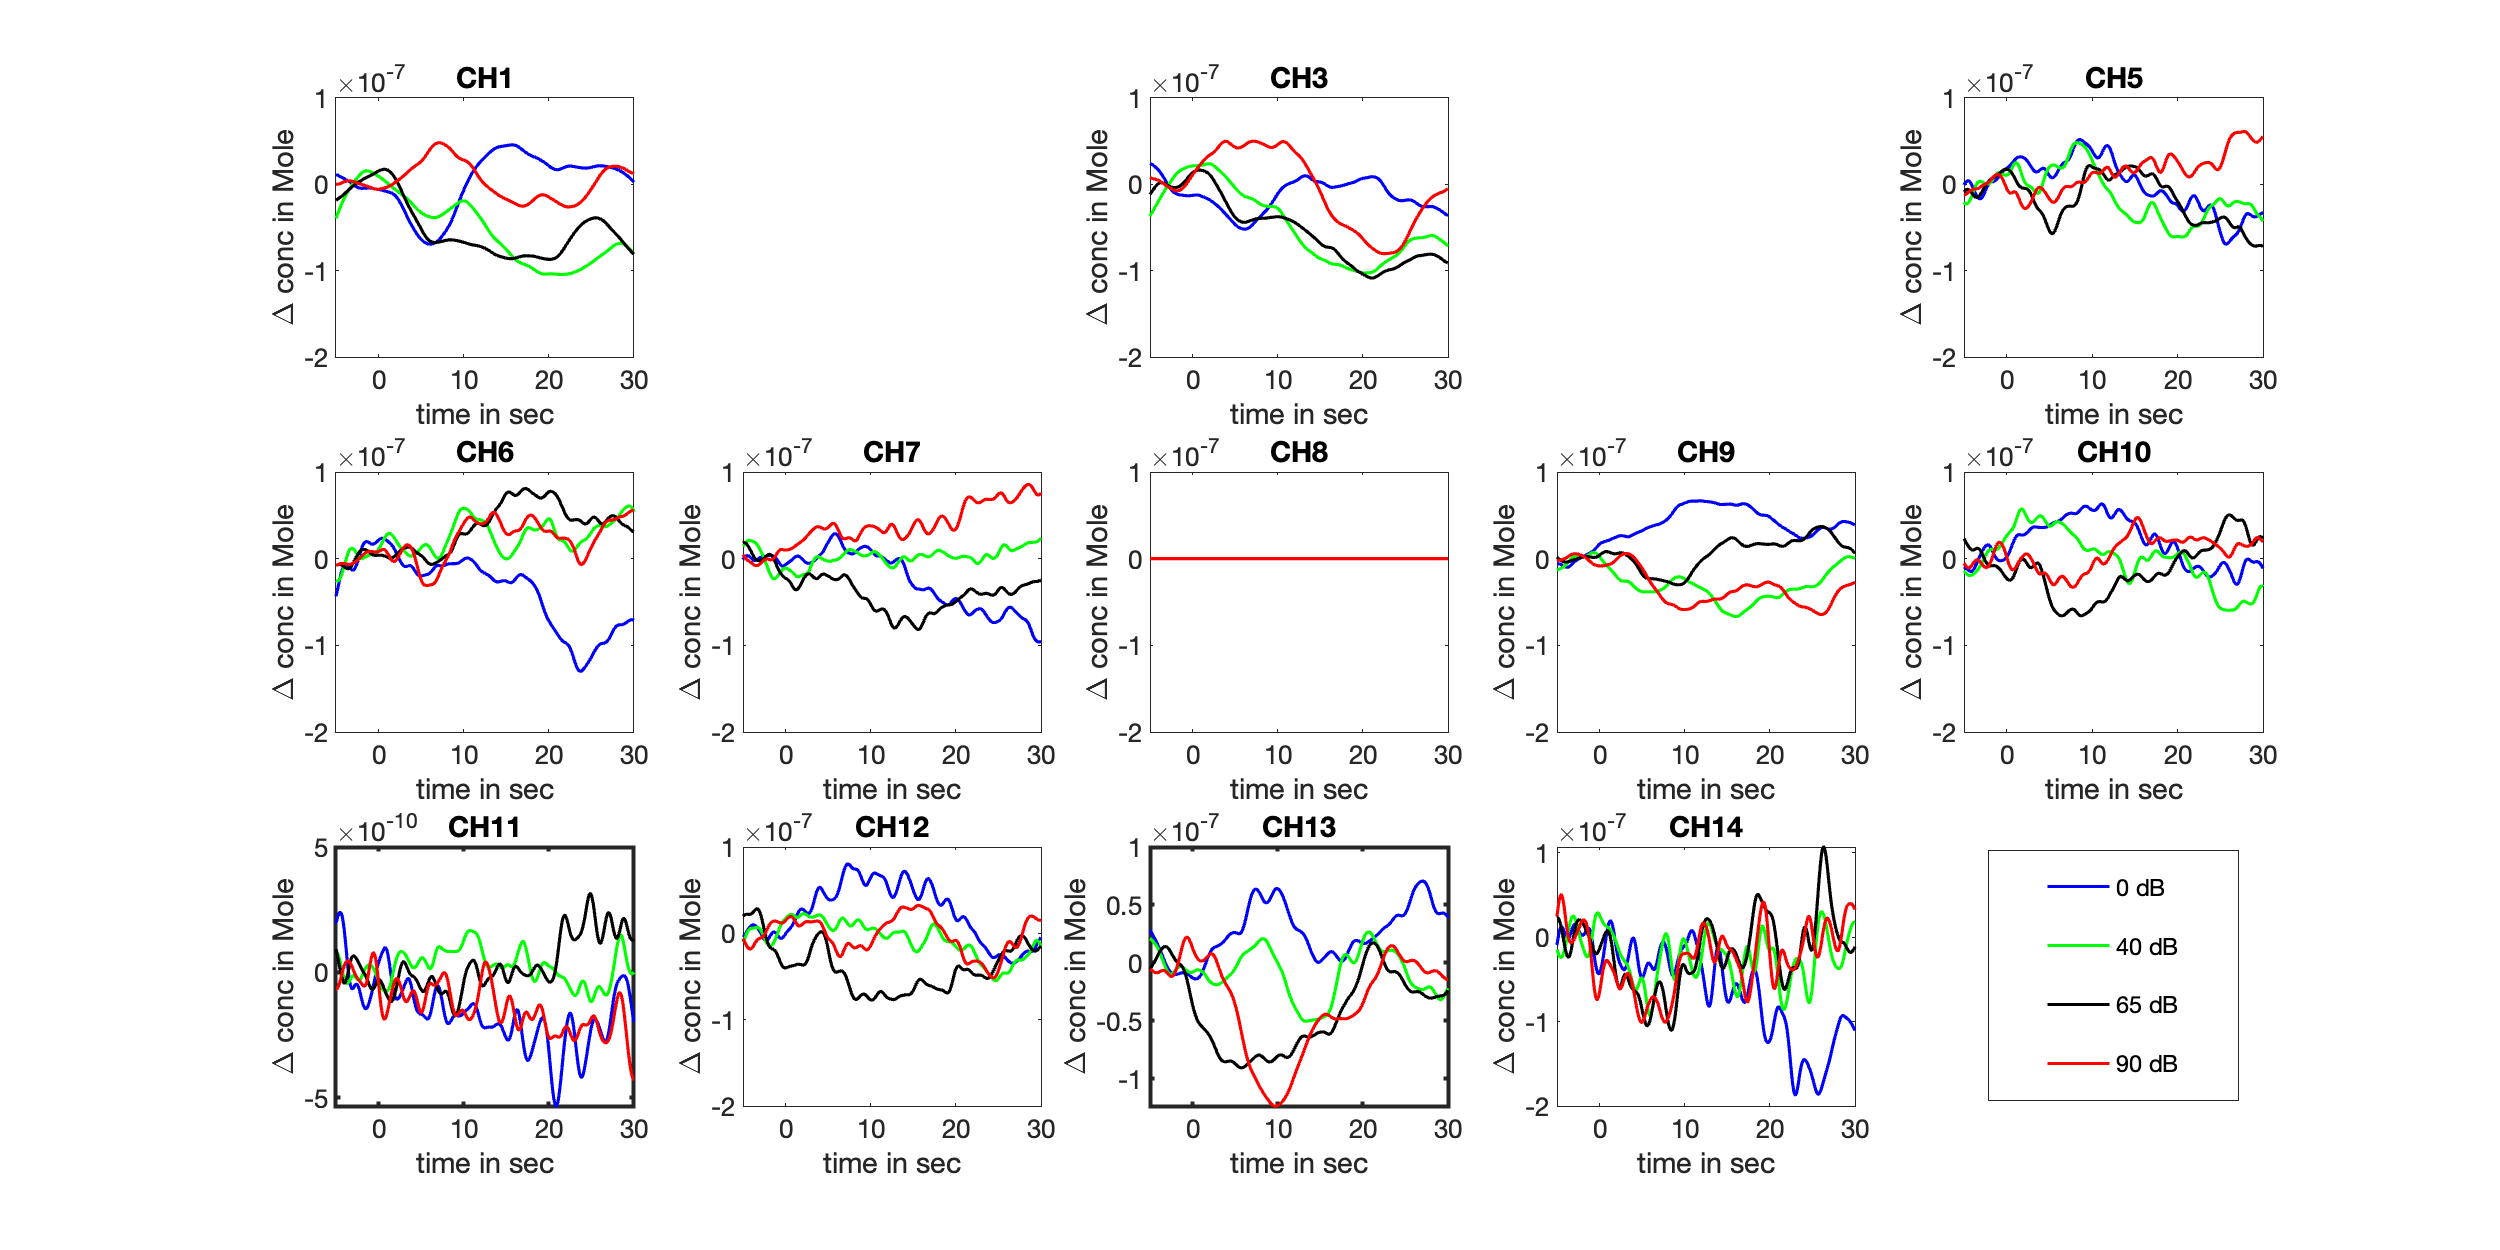
\includegraphics[scale=.4]{bilder/HbR_Mole/sub_shelia_s_HbR.png}
  \caption{Measurement from participant 6.}
  \label{fig:somesignal}
\end{figure}

\begin{figure}[H]
  \centering
    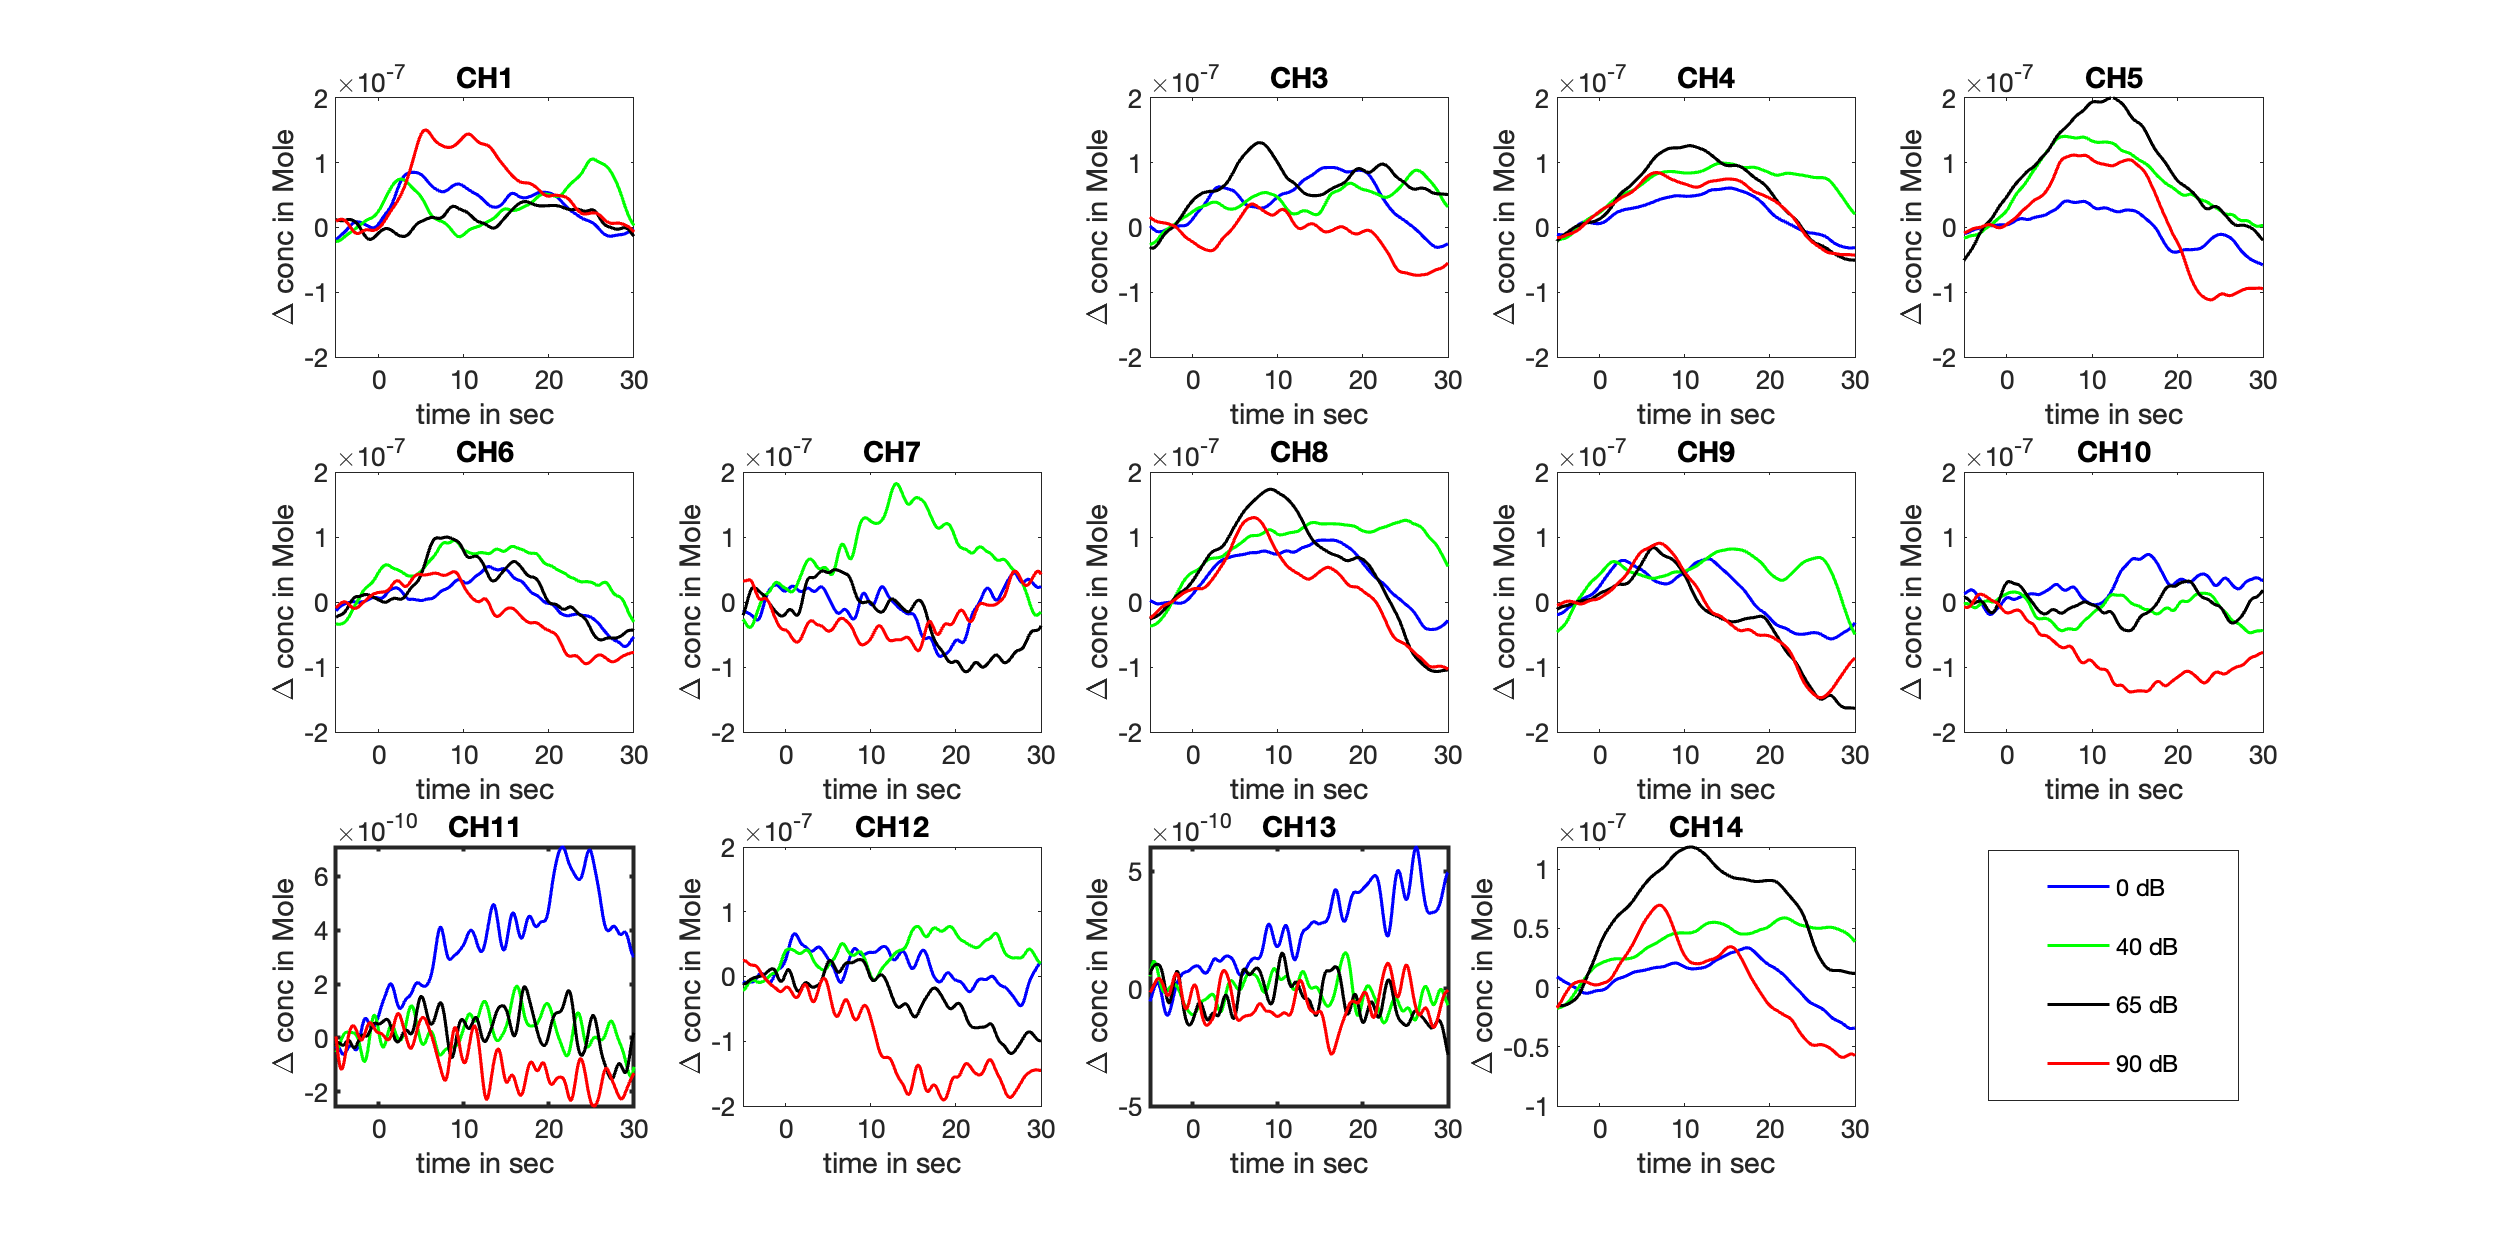
\includegraphics[scale=.4]{bilder/HbR_Mole/sub_liao_s_HbR.png}
  \caption{Measurement from participant 7.}
  \label{fig:somesignal}
\end{figure}


\begin{figure}[H]
  \centering
    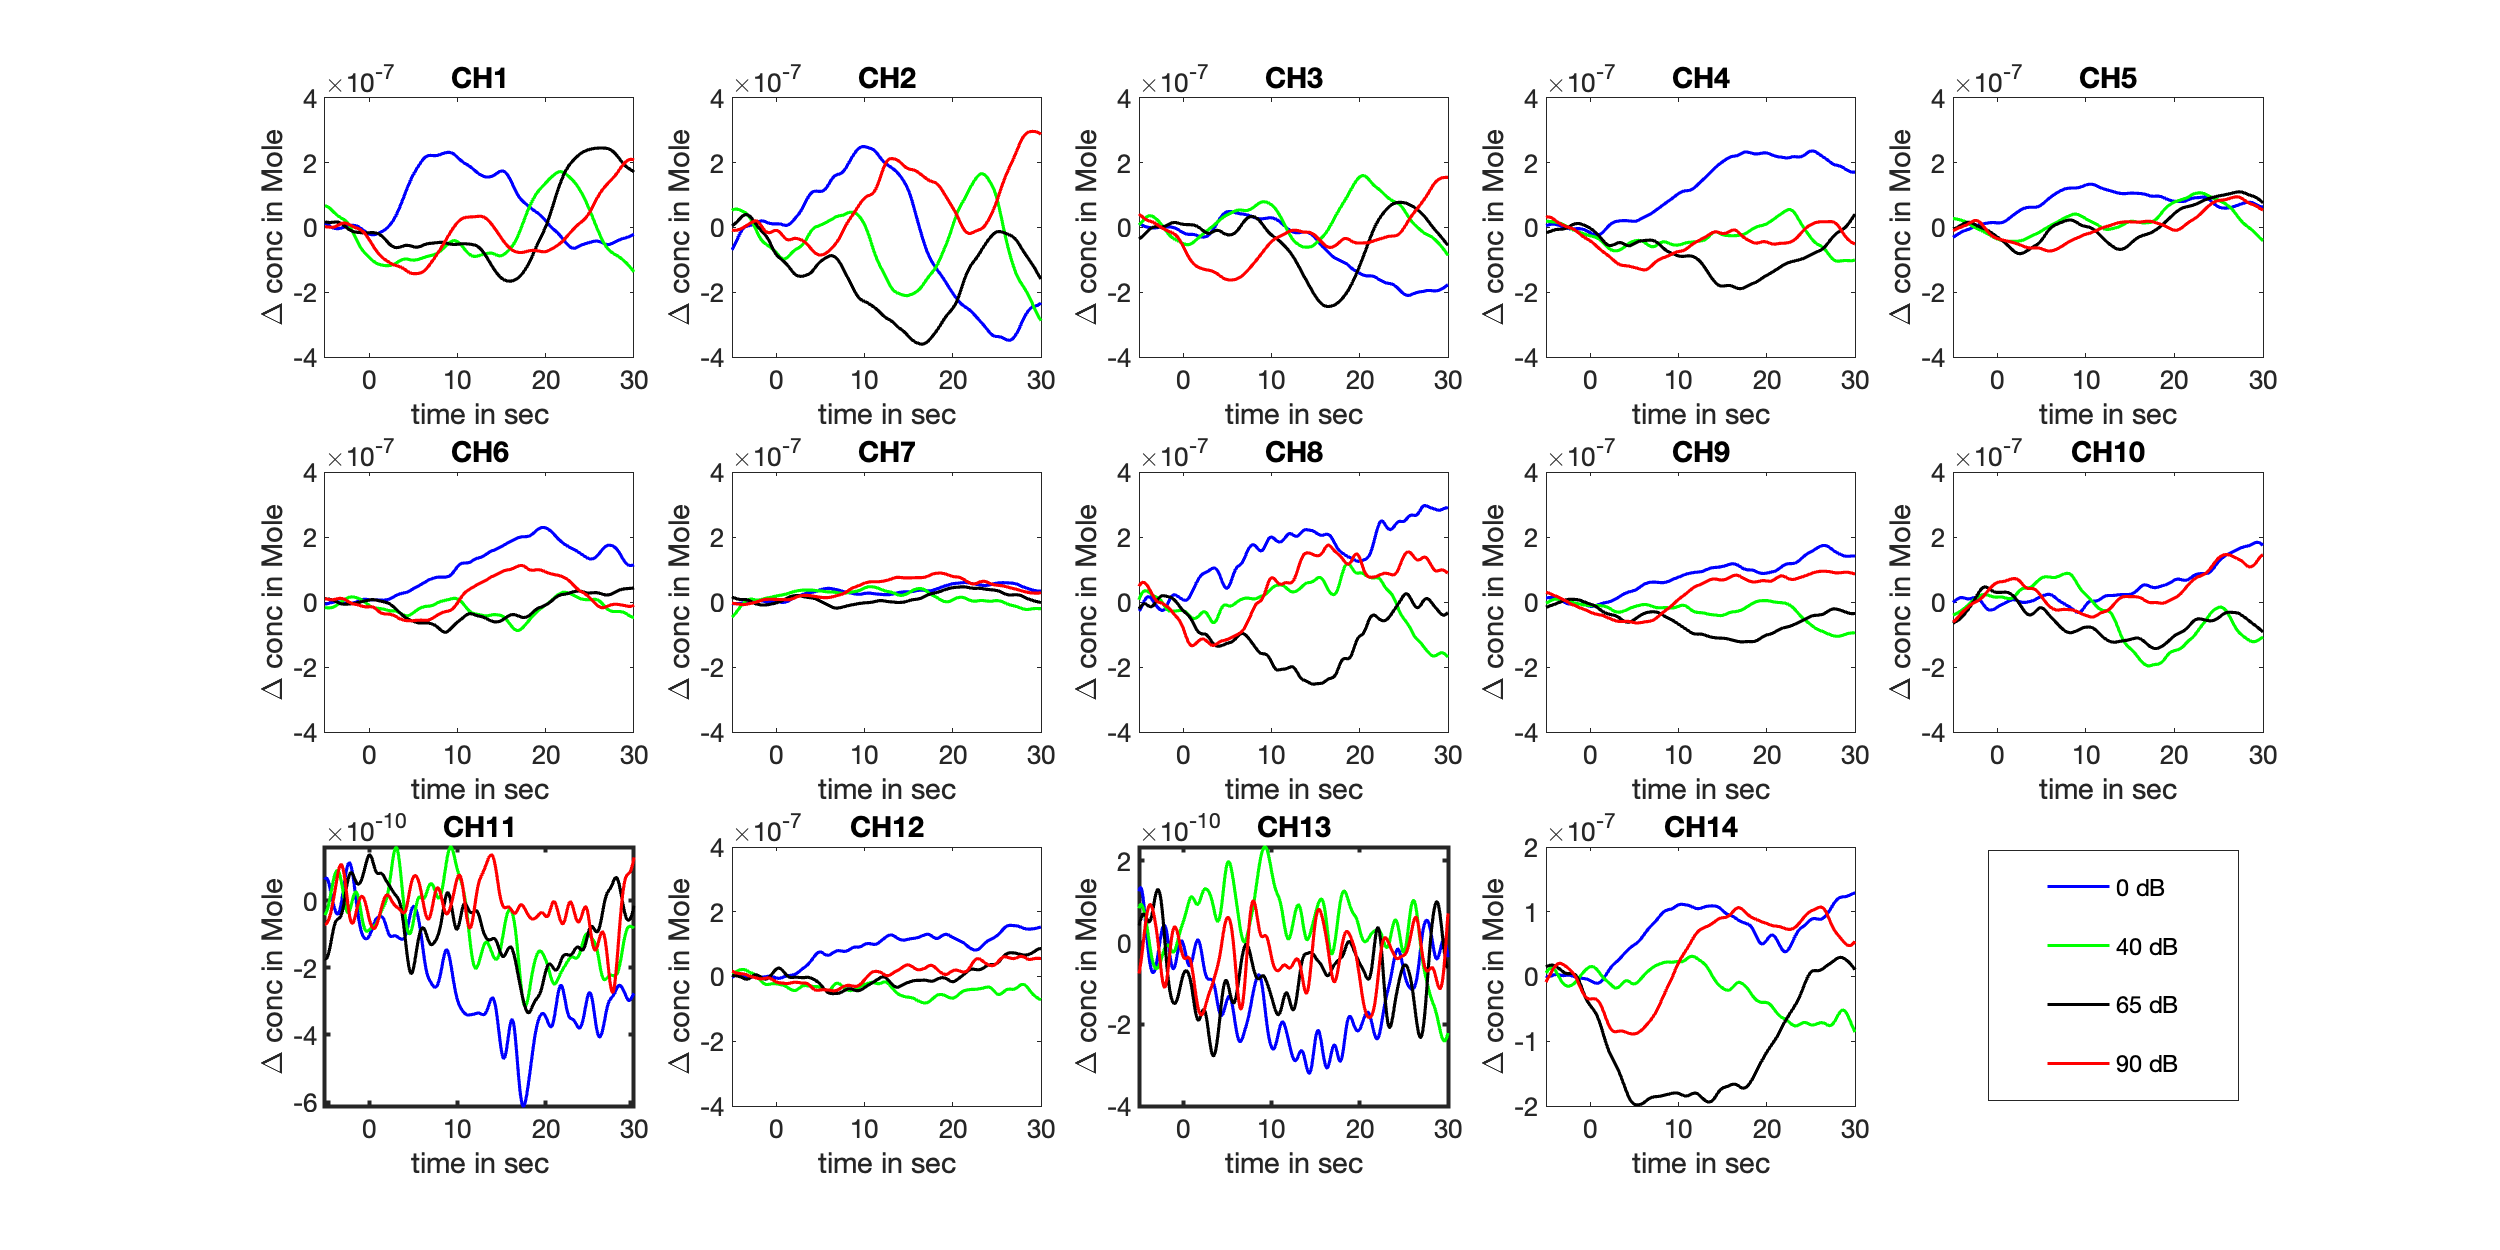
\includegraphics[scale=.4]{bilder/HbR_Mole/sub_luca2_s_HbR.png}
  \caption{Measurement from participant 8. Silent comparison}
\end{figure}





\section {Region of Interest}
In the following, regions of interest (ROI) are defined as the following figures. The auditory cortex is in particular of our interest. Hence, channel 4, channel 8, and channel 9 together formed one region (ROI 2). The rest of the channels formed ROI 1. It is of our interest to compare how the response of the auditory cortex differ from the rest of the left brain hemisphere.

\begin{figure}[H]
  \centering
    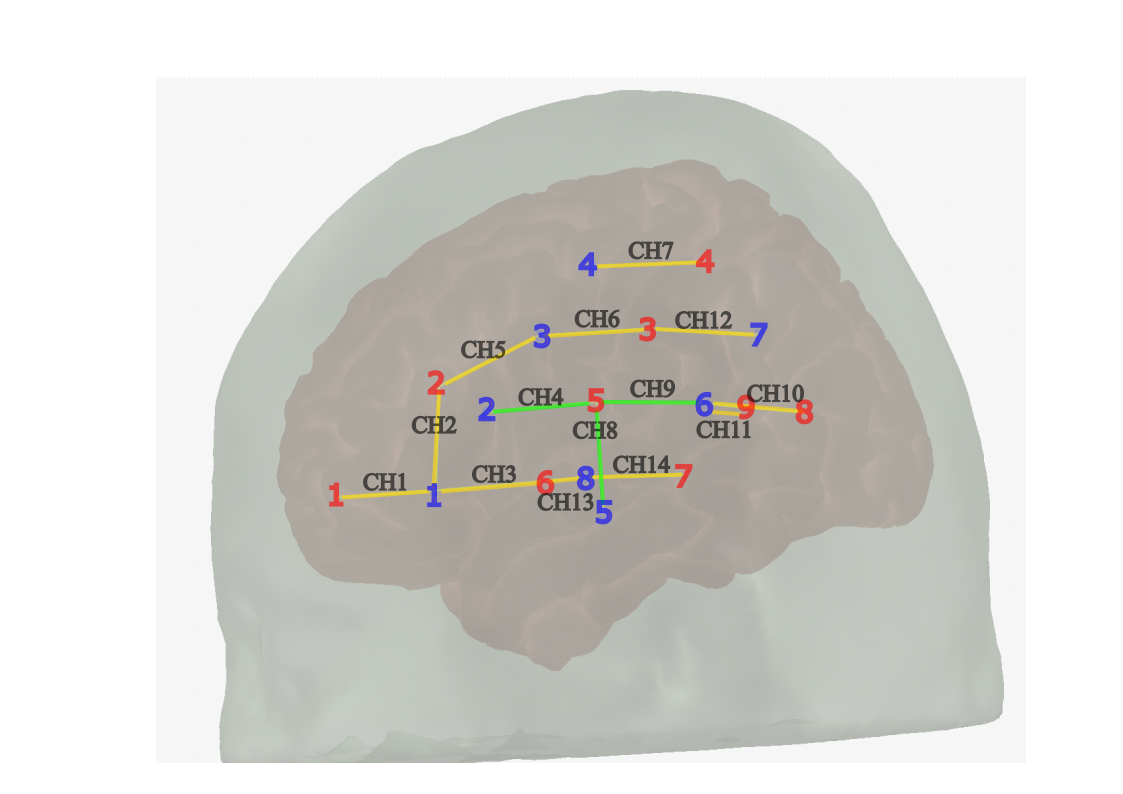
\includegraphics[scale=.45]{bilder/optode_roi_ink.png}
  \caption{ROI Definition}
\end{figure}



The following plots shows the averaged \textbf {HbO} response of all the valid channels in the defined region.
\begin{figure}[H]
  \centering
    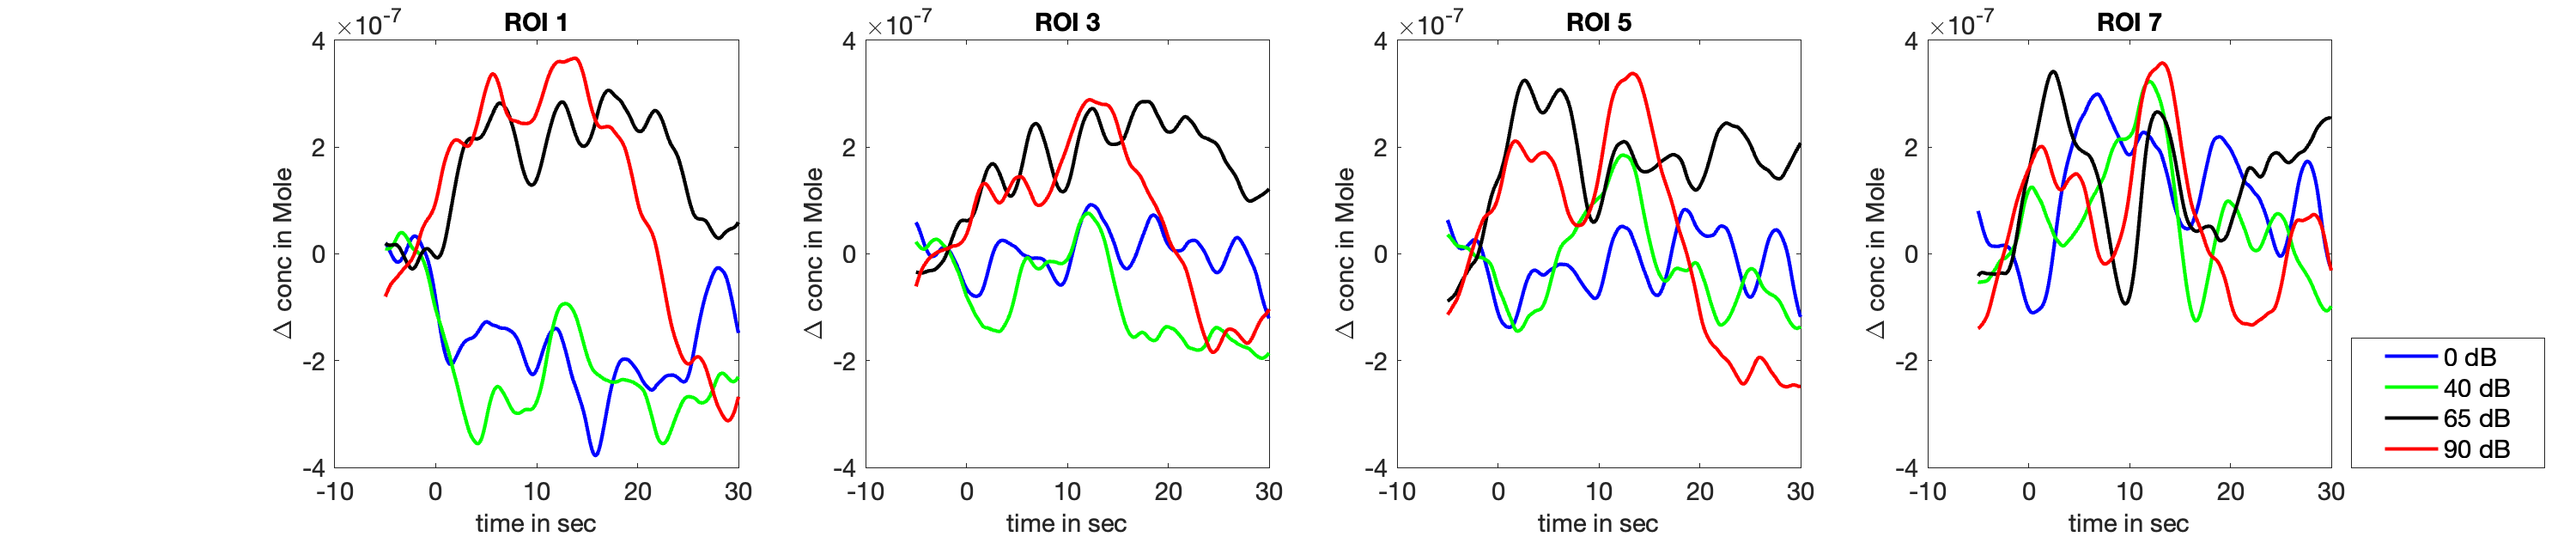
\includegraphics[scale=.29]{bilder/ROI/sub_chang_s_HbO.png}
  \caption{Measurement from participant  1.}
\end{figure}

\begin{figure}[H]
  \centering
    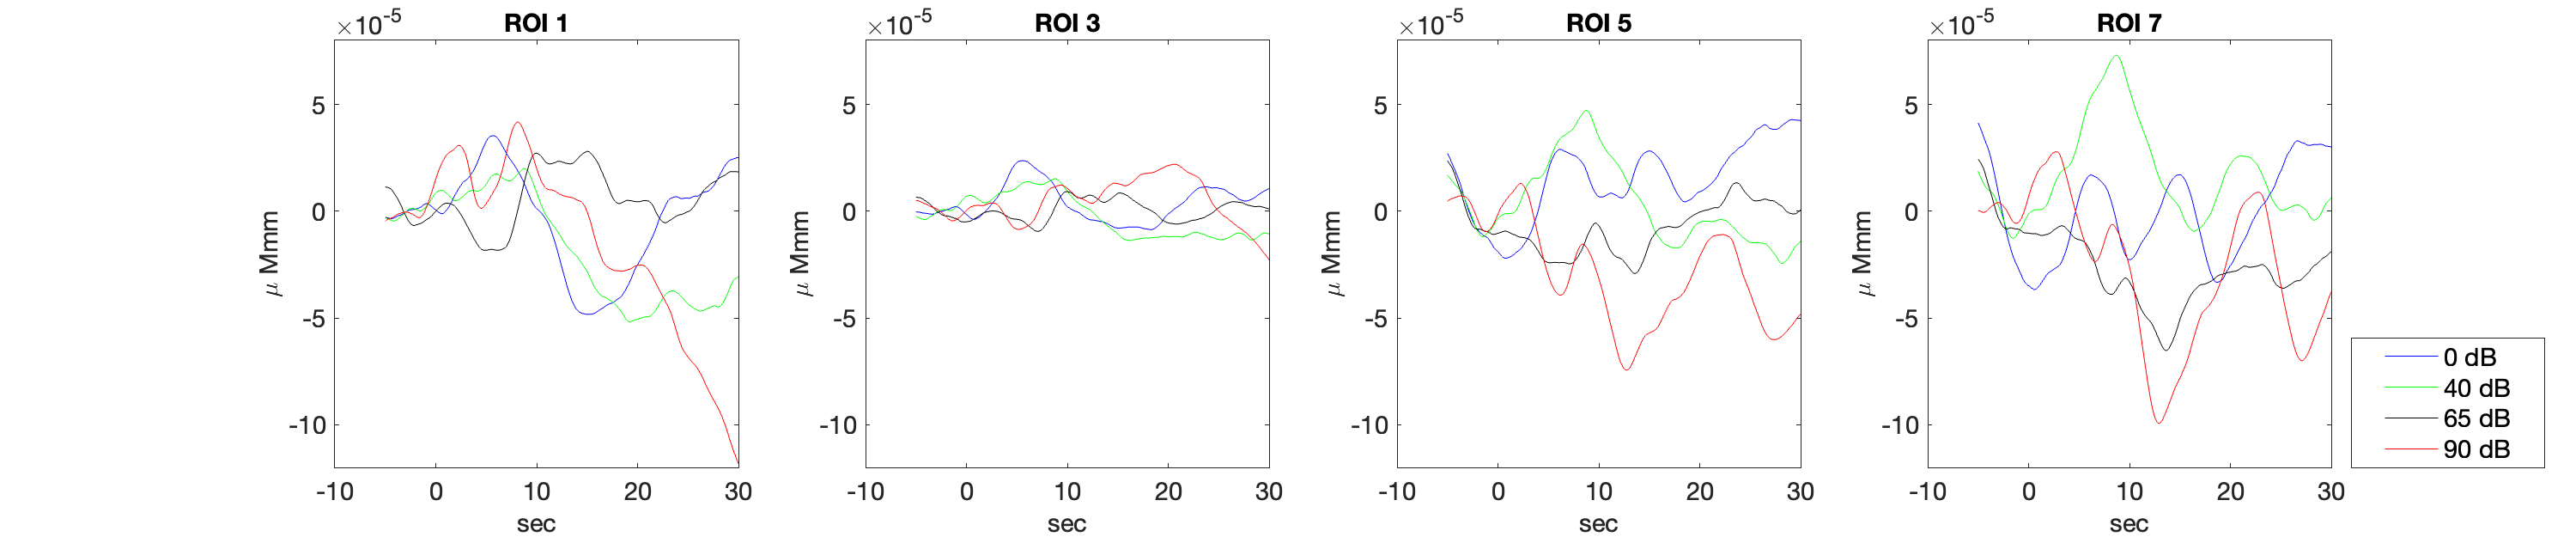
\includegraphics[scale=.29]{bilder/ROI/sub_gleb2_s_HbO.png}
  \caption{Measurement from participant  2.}
\end{figure}

\begin{figure}[H]
  \centering
    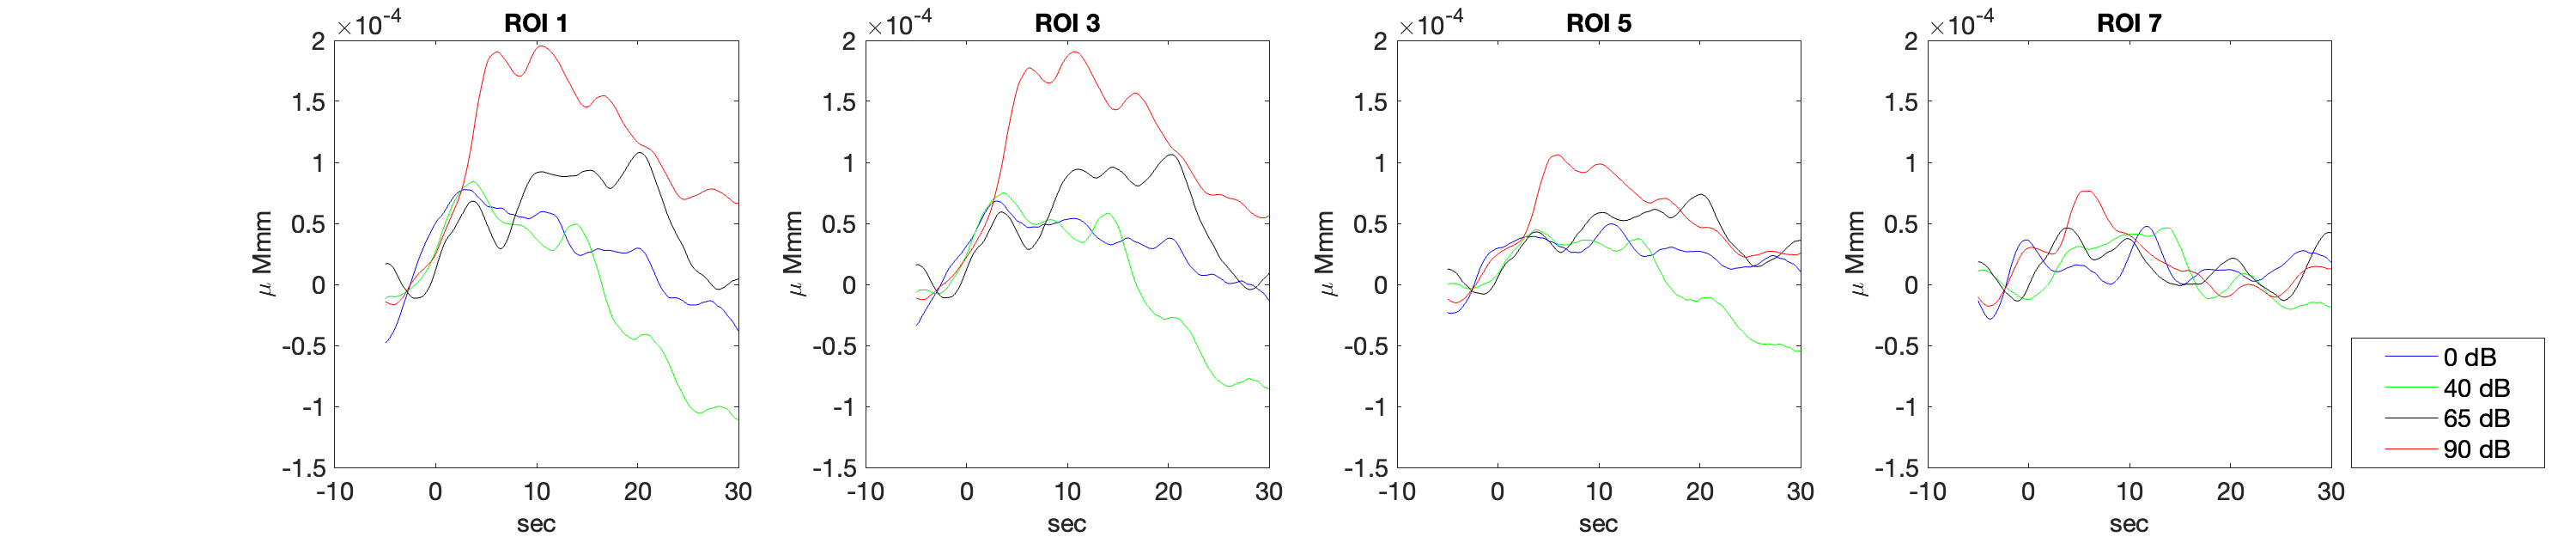
\includegraphics[scale=.29]{bilder/ROI/sub_jonas_s_HbO.png}
  \caption{Measurement from participant  3.}
\end{figure}

\begin{figure}[H]
  \centering
    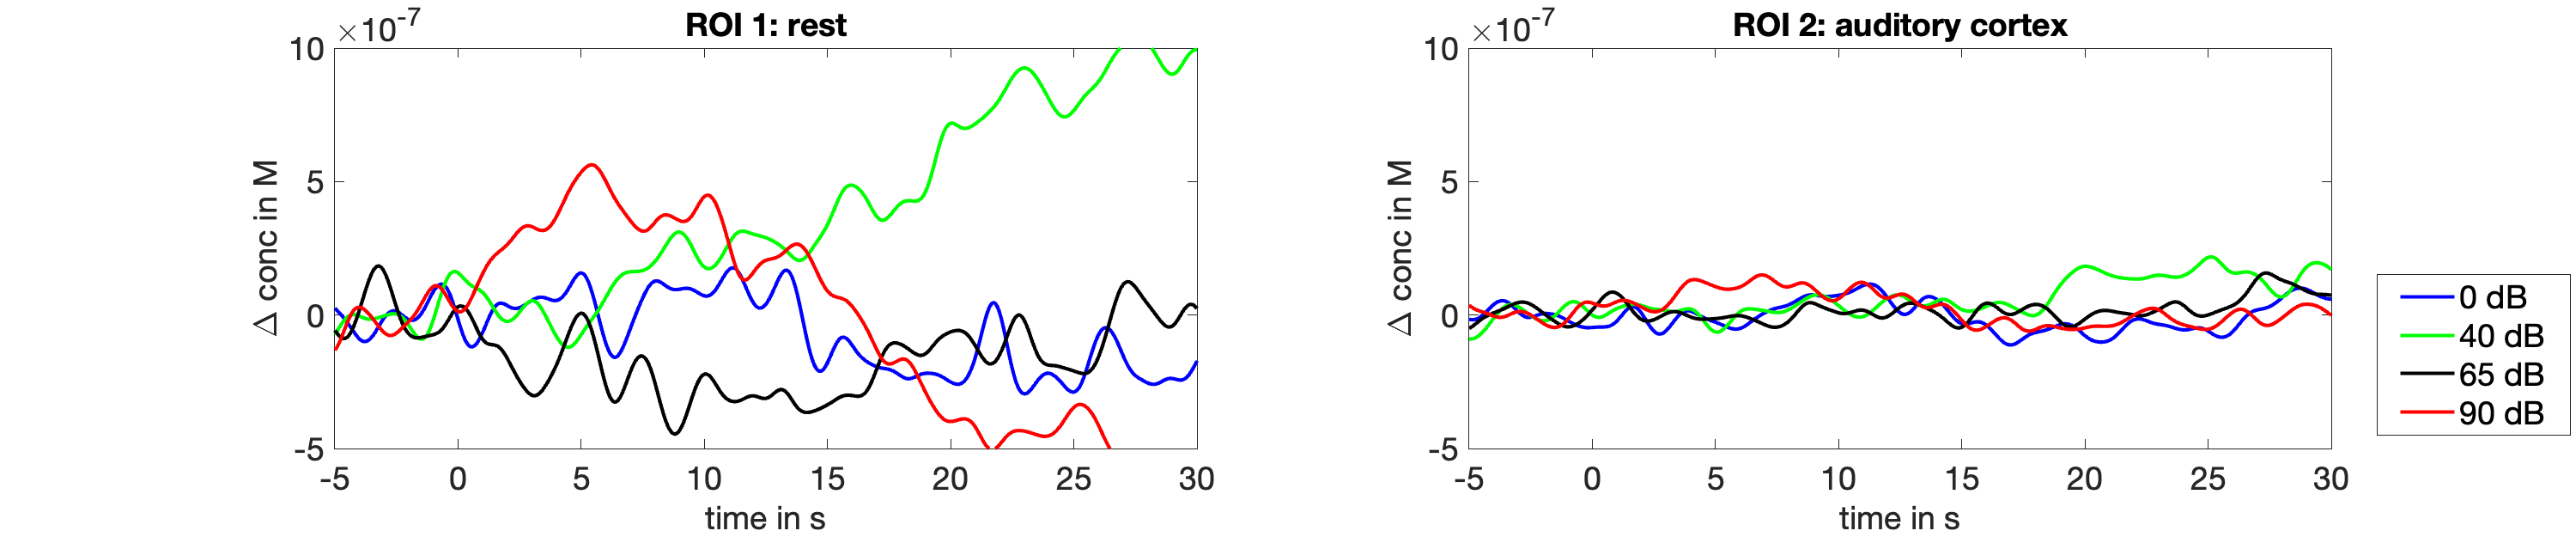
\includegraphics[scale=.29]{bilder/ROI/sub_lin_s_HbO.png}
  \caption{Measurement from participant  4.}
\end{figure}

\begin{figure}[H]
  \centering
    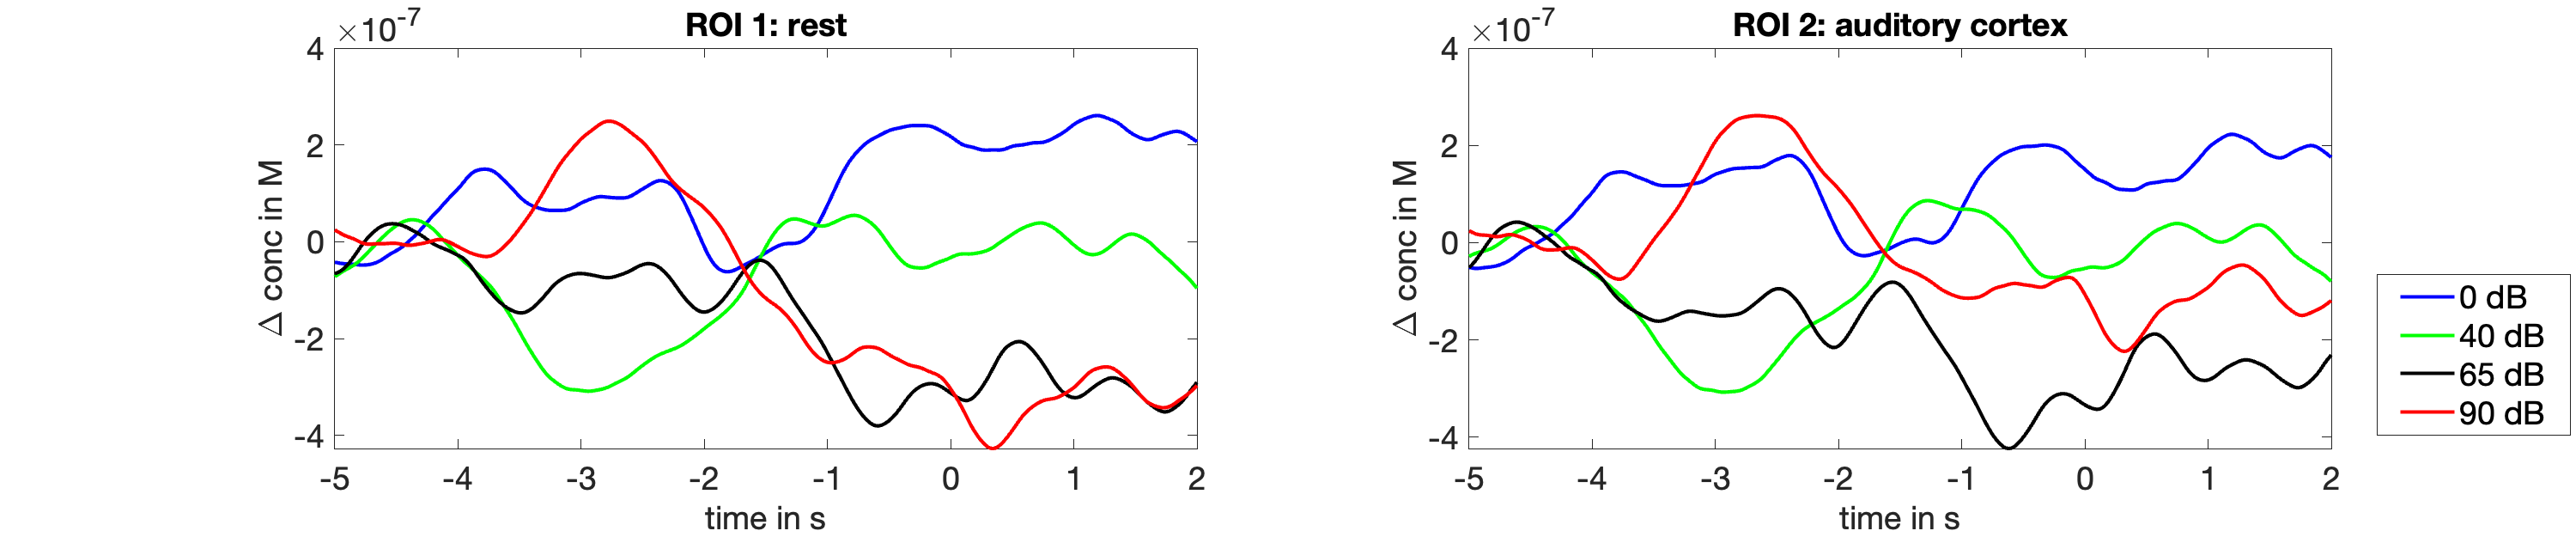
\includegraphics[scale=.29]{bilder/ROI/sub_lukas_s_HbO.png}
  \caption{Measurement from participant 5.}
\end{figure}

\begin{figure}[H]
  \centering
    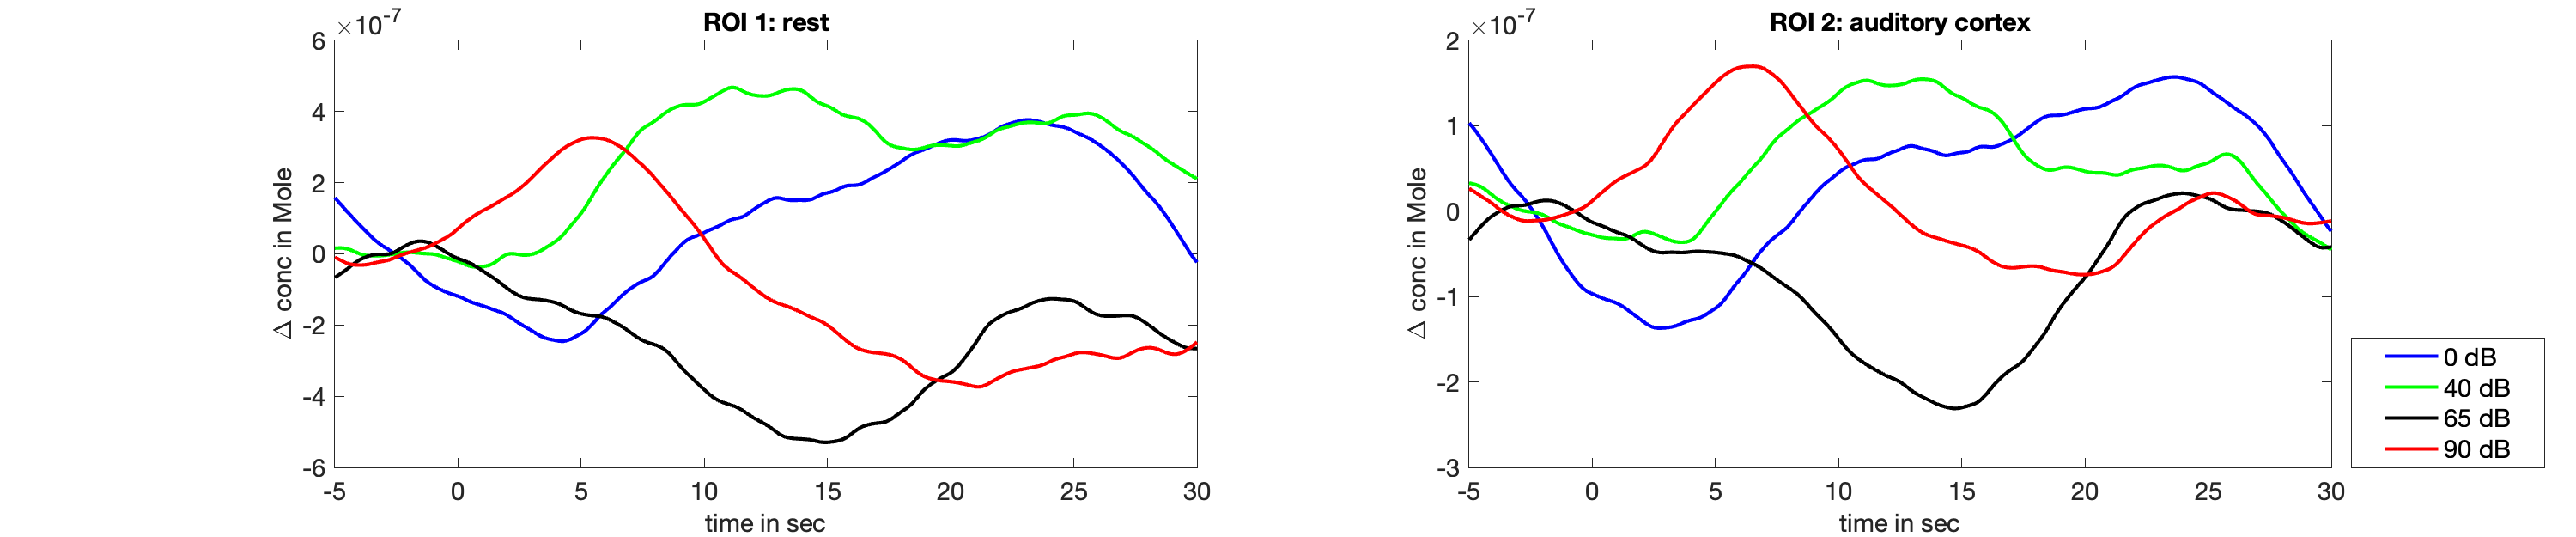
\includegraphics[scale=.29]{bilder/ROI/sub_shelia_s_HbO.png}
  \caption{Measurement from participant  6.}
\end{figure}


\begin{figure}[H]
  \centering
    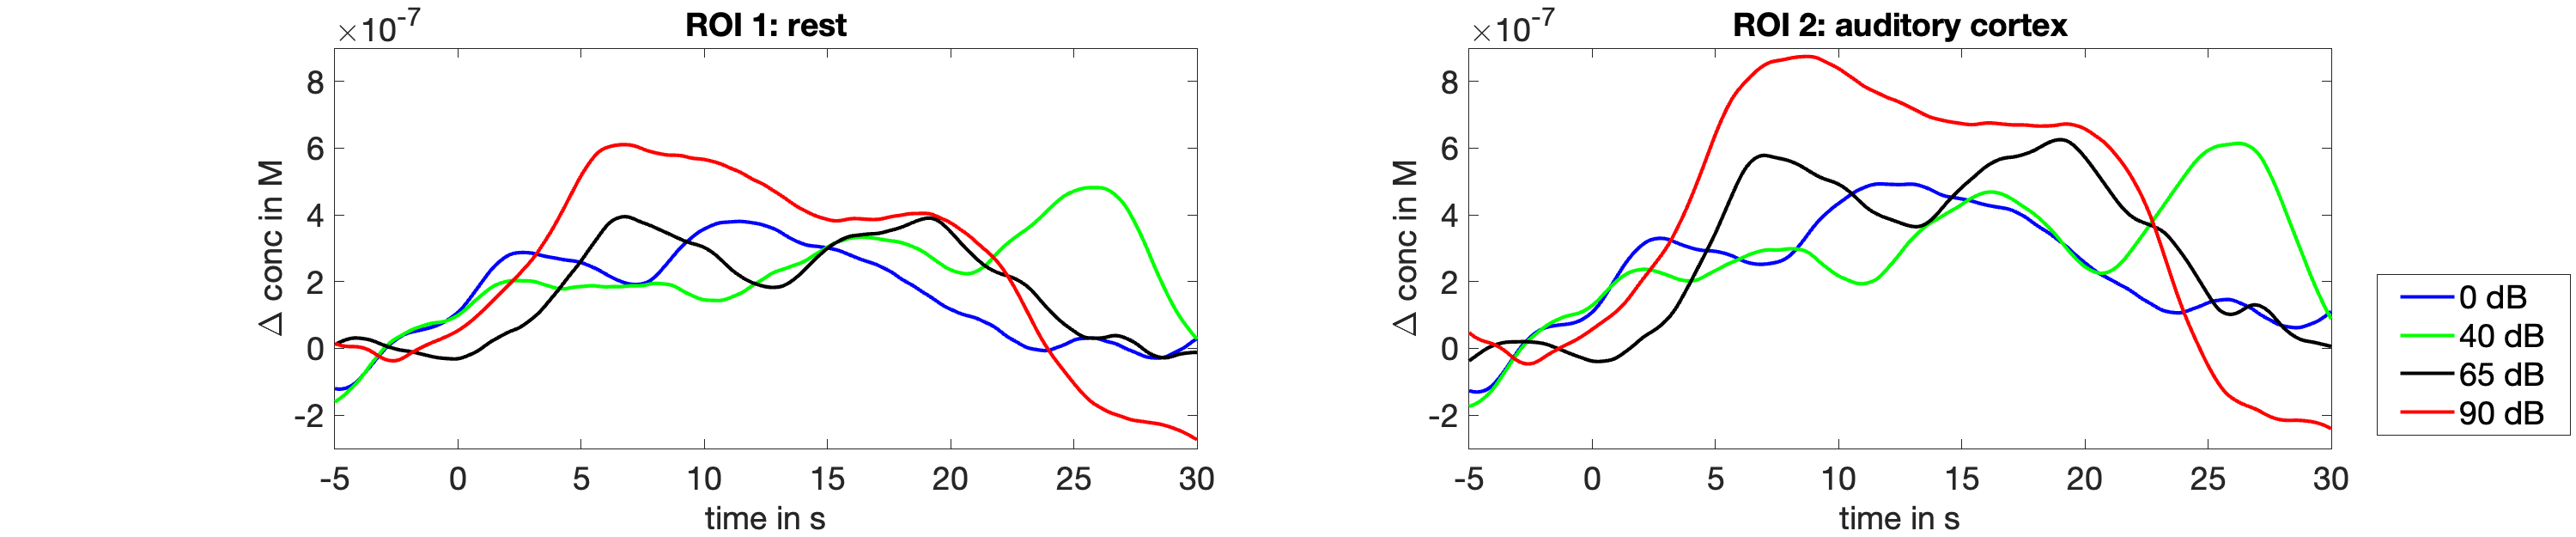
\includegraphics[scale=.29]{bilder/ROI/sub_liao_s_HbO.png}
  \caption{Measurement from participant 7.}
\end{figure}



\begin{figure}[H]
  \centering
    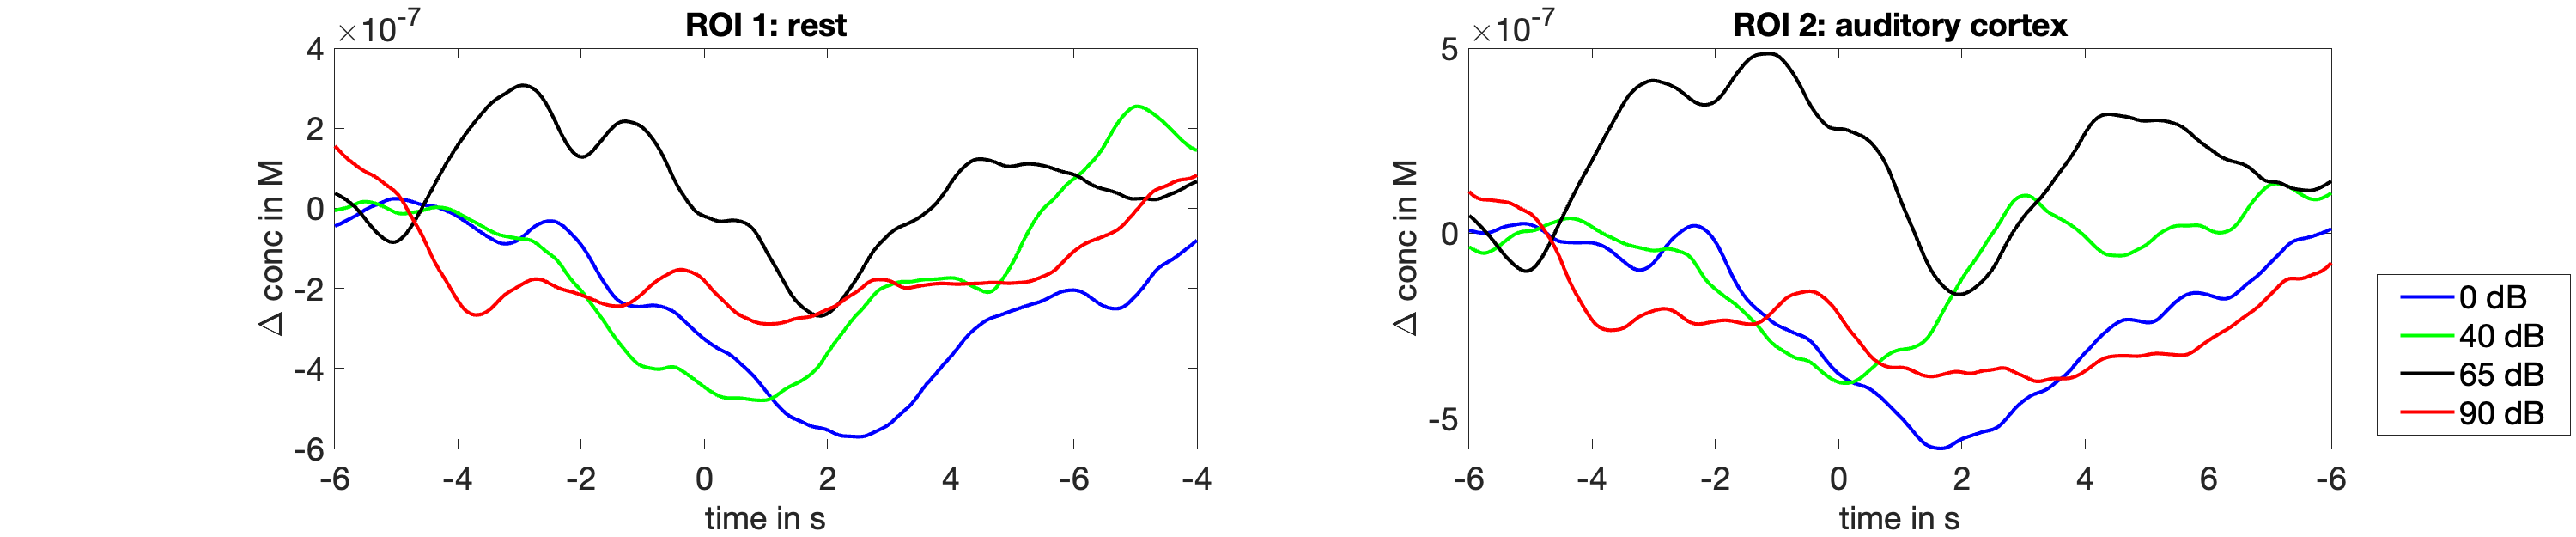
\includegraphics[scale=.29]{bilder/ROI/sub_luca2_s_HbO.png}
  \caption{Measurement from participant 8. Silent comparision.}
\end{figure}

\newpage

\section {Poor Measurements}
There were also some poor measurements even though the SCI is above the threshold 0.75. For example, in our case of participant 4. One possible reason can be due to the thick dark hair of the participant. Light absorption can affect the result greatly.

\begin{figure}[H]
  \centering
    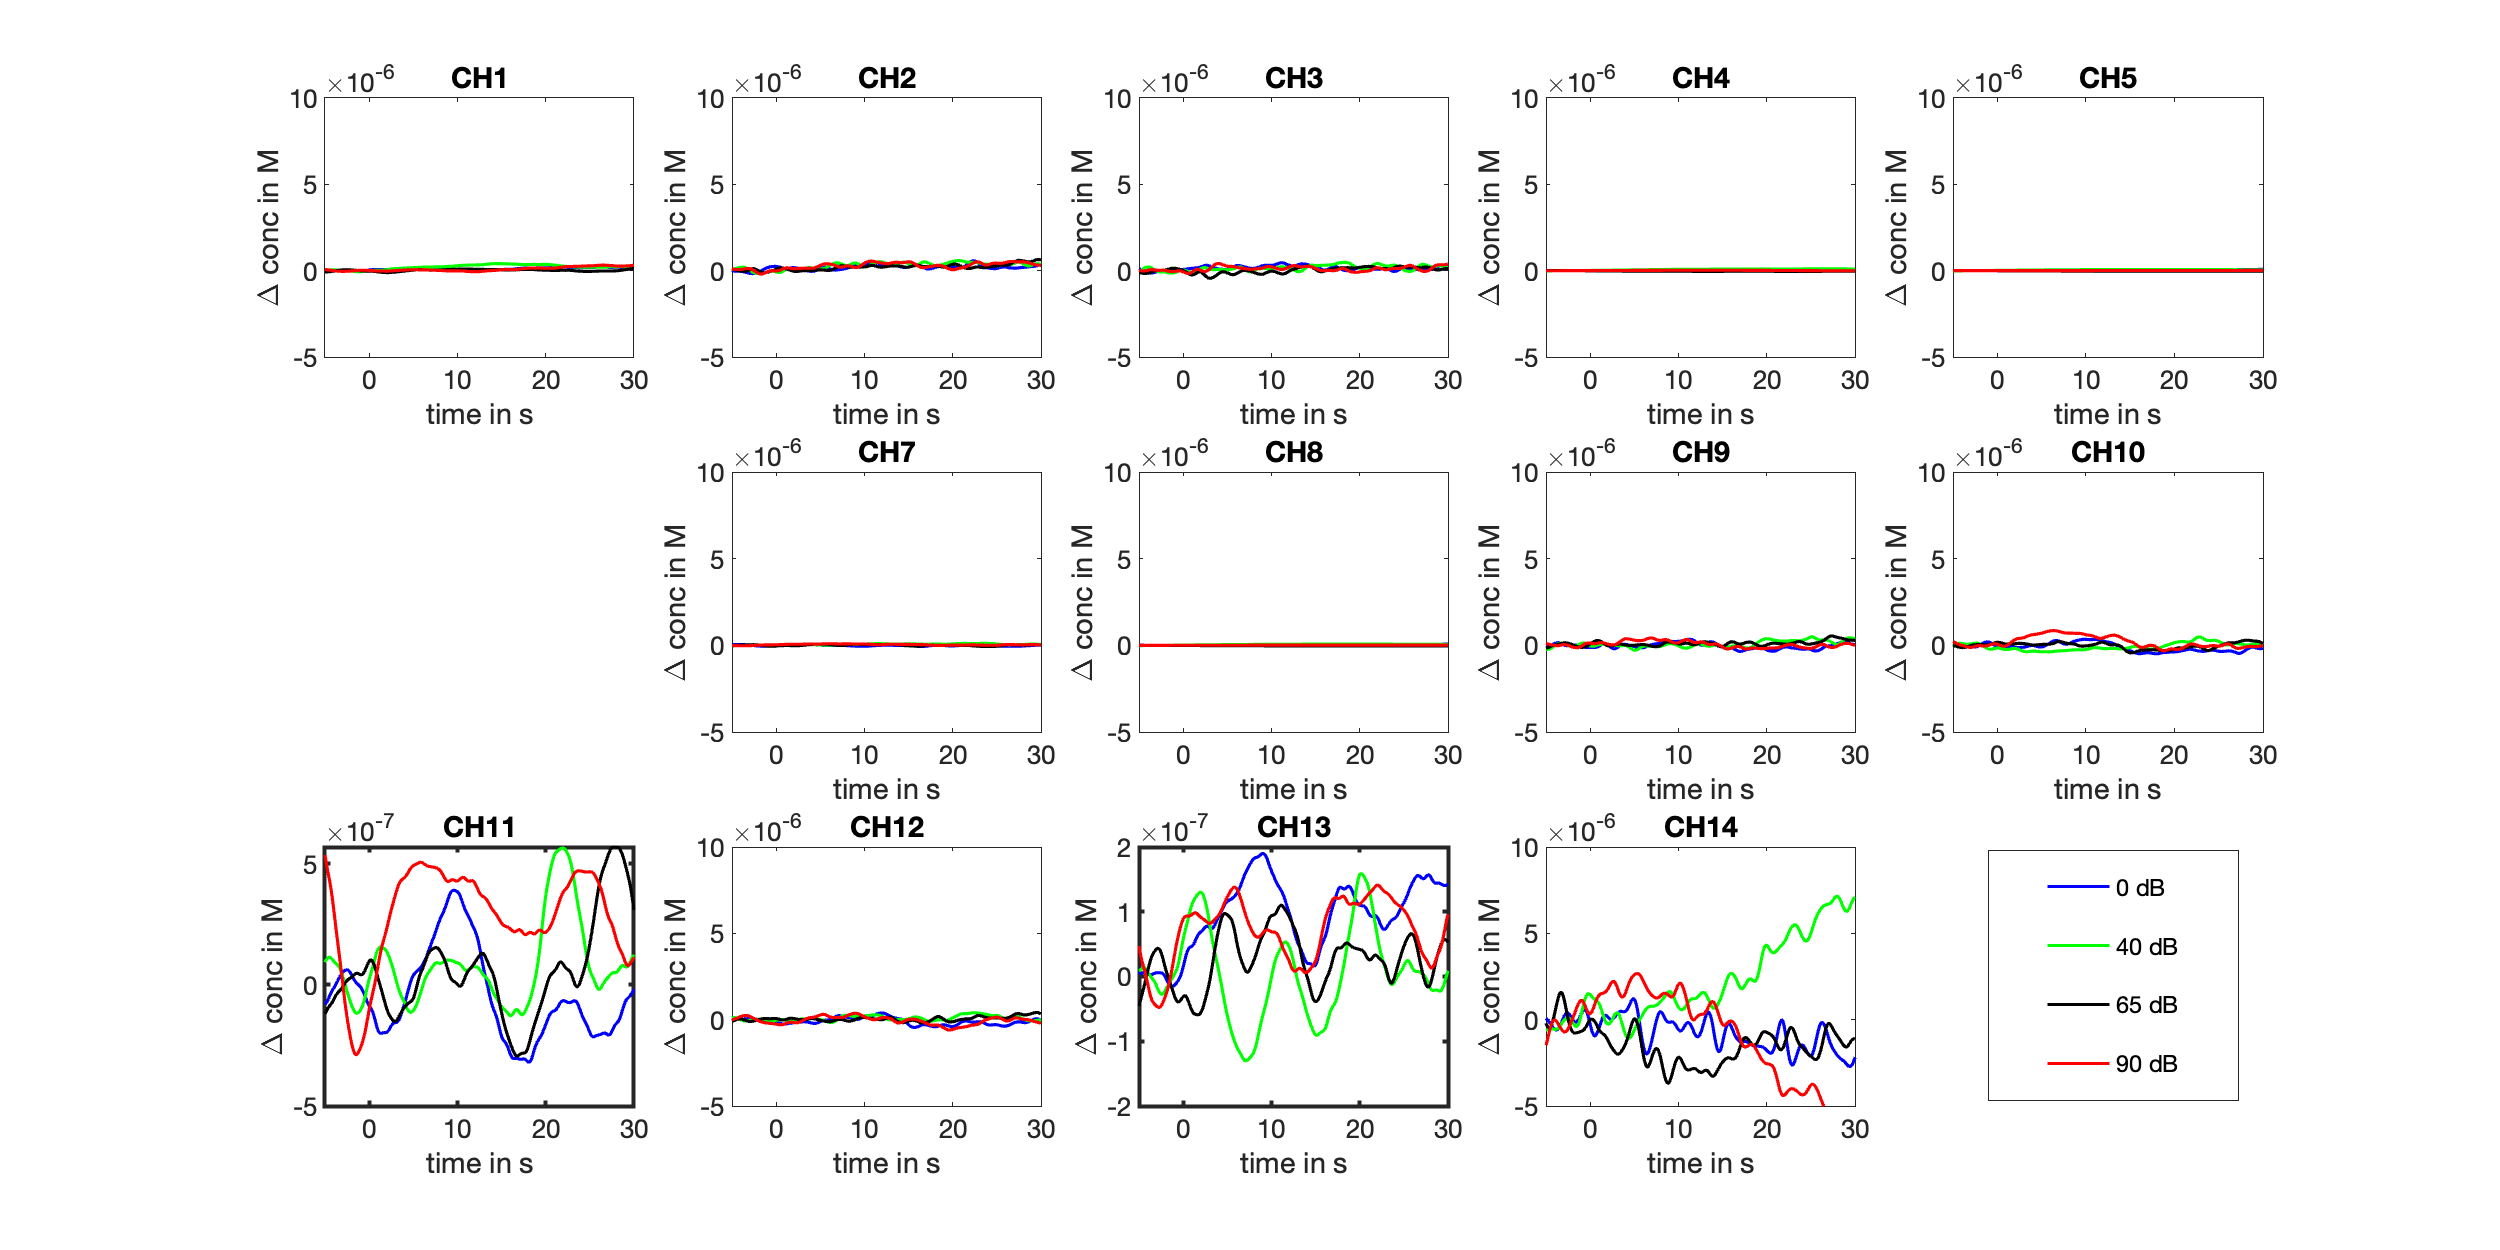
\includegraphics[scale=.35]{bilder/HbO_Mole/sub_lin_s_HbO.png}
  \caption{HbO Measurement from participant 4.}
\end{figure}


\begin{figure}[H]
  \centering
    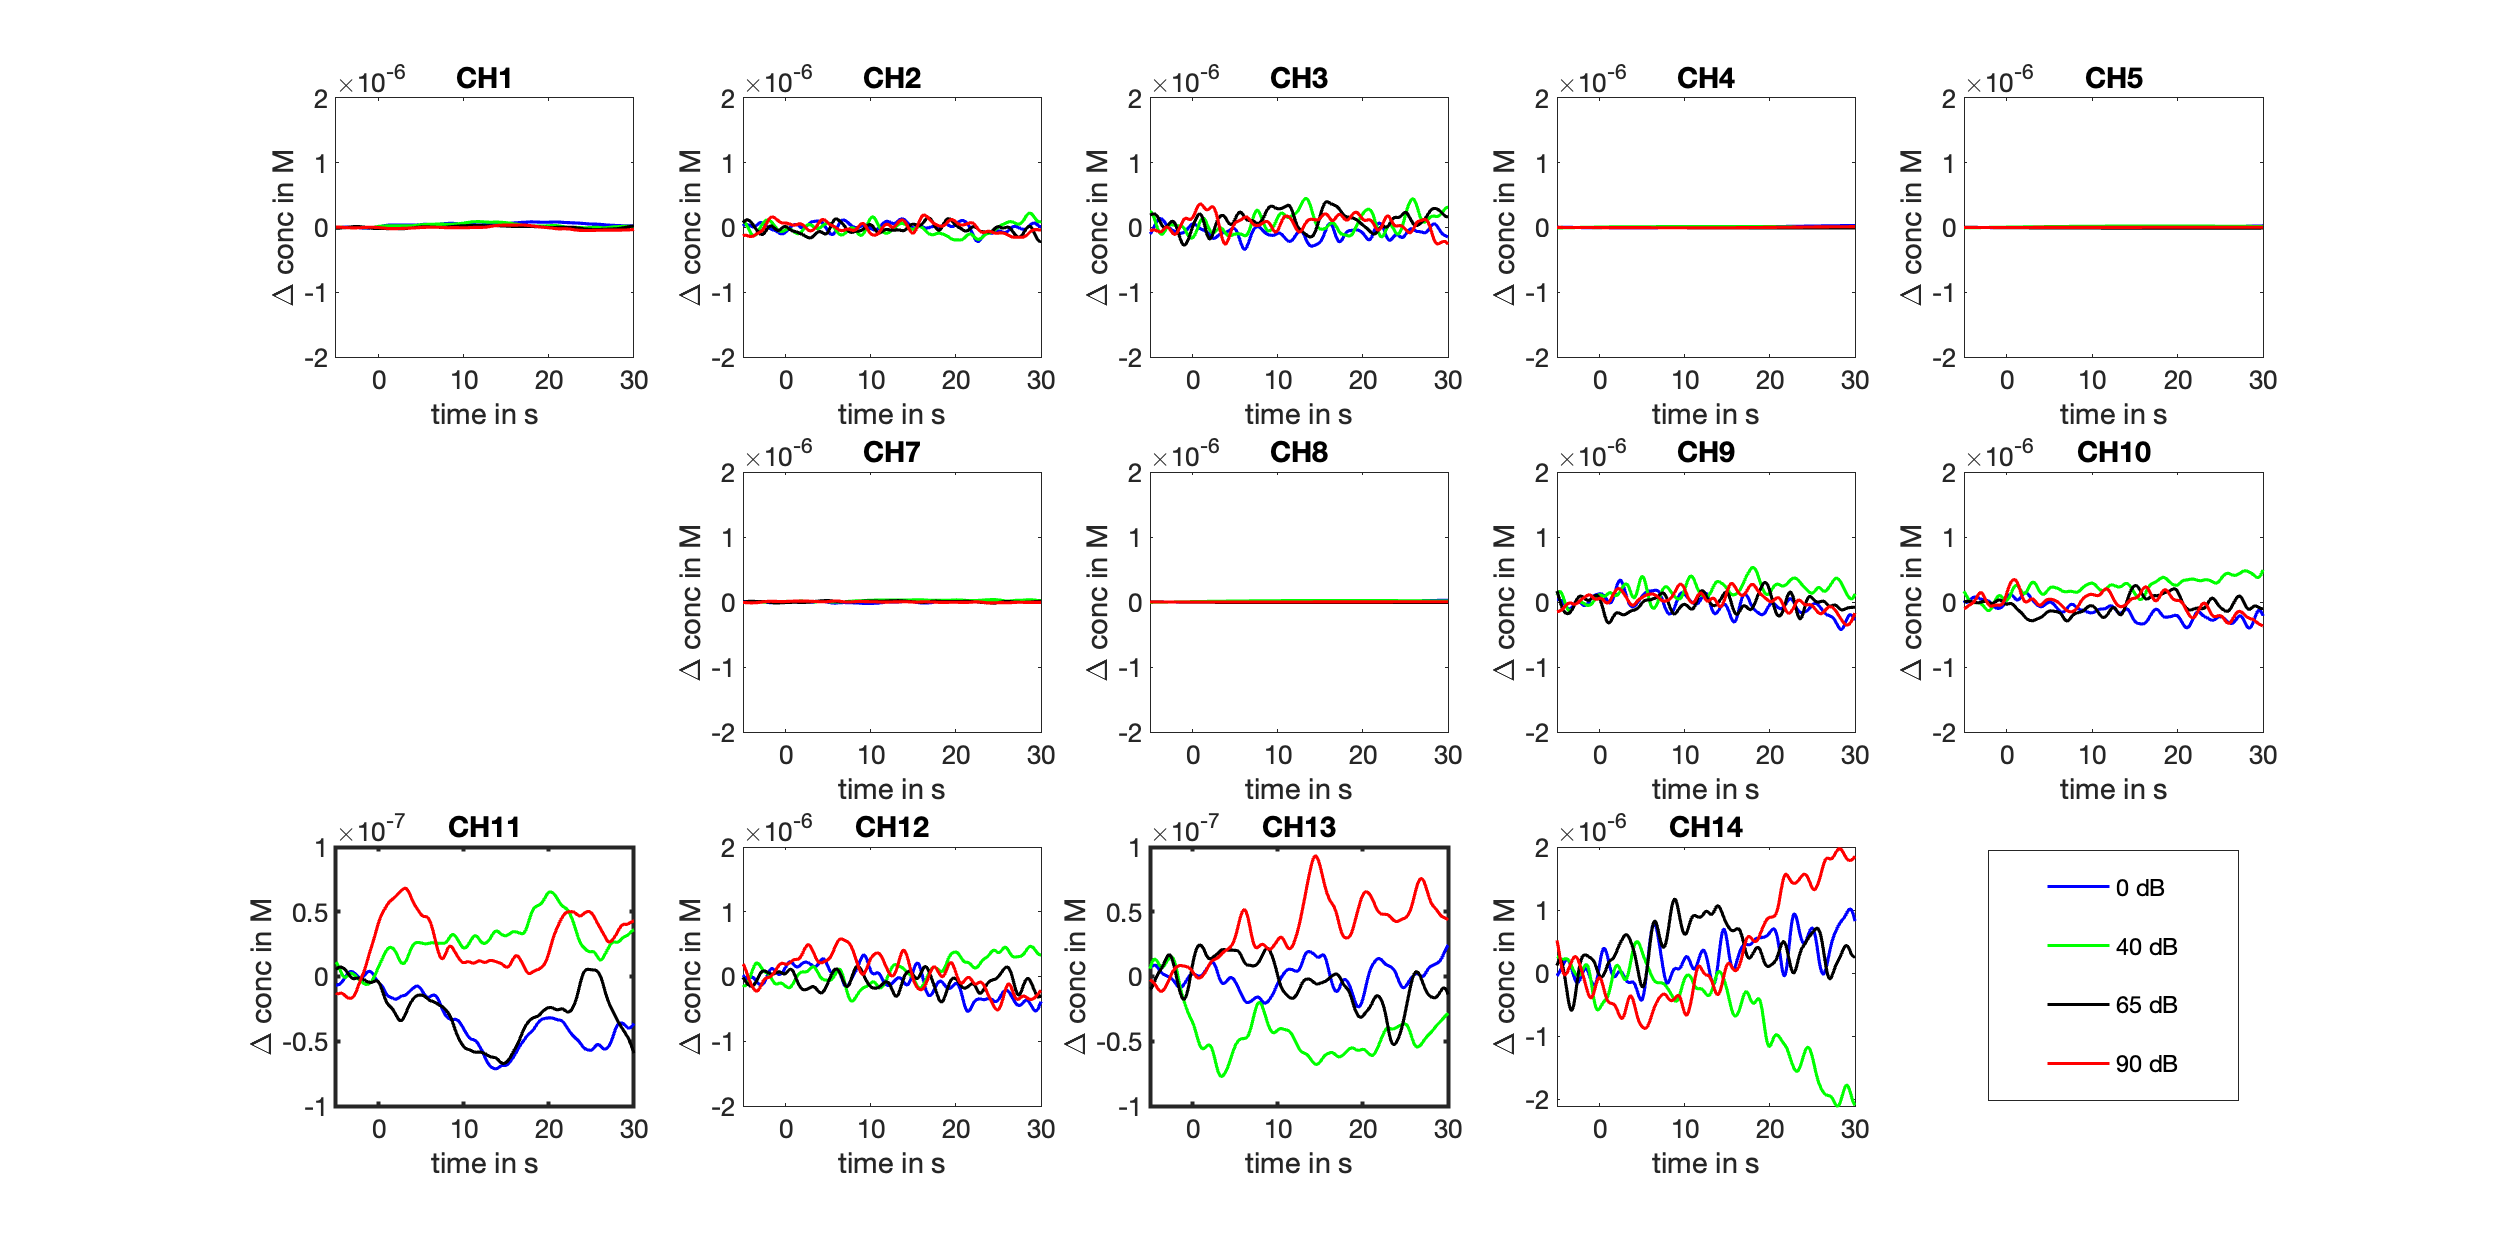
\includegraphics[scale=.35]{bilder/HbR_Mole/sub_lin_s_HbR.png}
  \caption{HbR Measurement from participant 4.}
\end{figure}


\chapter{Discussion}
In this chapter, individual case-by-case study will be discussed in detail. The results from our measurements will also be compared with the counterparts form Weder et al.

\section {Participant 3}
The results from this participant was the closest one to the results reported by Weder et al. For the oxygenated hemoglobin HbO waveform morphology, tonic response could be observed in channel 1, 2, and 3, and phasic response could be observed in channel 10 and 12.

\section {Participant 5}
For the oxygenated hemoglobin HbO waveform, there were significantly larger on-sets for the 90 dB sound stimuli in Channel 1, 2, and 3, i.e. around the Broca's area.

Apart from this, the waveforms for deoxygenated hemoglobin, HbR, were also quite different from the ones Weder et al. reported. For the loudest sound stimuli, channels overlying the caudal superior temporal gyrus and channels over Broca's area showed clear phasic response. 

\section {Participant 6}

For the oxygenated hemoglobin, HbO waveform, the loudest sound stimuli resulted in phasic response for almost all the channels. In addition, it also resulted in faster on-set compared with other stimuli of lower sound pressure levels.

On the other hand, as for the deoxygenated hemoglobin, HbR response, results from multiple channels appeared to be noisy even if the SCI values were already above the suggested threshold.


\section {Participant 7}

The results from this participant are rather indeterminant to differentiate between response to different sound pressure levels.


\section {Participant 8}
This participant was given only silence stimuli. No pattern could be concluded for the measured waveform morphology. Nonetheless, it's noteworthy to know that even if there are almost no visual and sound stimuli, dynamic hemoglobin response still exists.
\chapter{Conclusion and Future Prospectives}
//conclusion
In this project, we aimed to confirm and reproduce the results from Weder et al. With limited devices, we made our measurement conditions, i.e. optode template configuration and audio sound stimuli as similar as those of the previous research from Weder et al. as possible.

data processing
-> almost
->still not yet mentioned the beta and short channel extra cebrelle thingy
->dpf

waveform 

roi

//future

what could have gone wrong:
software different
cap position (optode template design and offsets when putting on a cap) mention the broca's area having phasic response (jonas?)

different device, different wavelength

more participants

better understanding of the spatial position with the optode templates (e.g. which channels are over brocas area, which are over supramarginal or caudal superior temporal gyrus, etc.

%%% Appendix
\appendix{}
%
\chapter{Important equation}
\label{cha:important-equation}

\begin{equation}
  \label{eq:1}
  \lim_{n \to \infty} \sum_{k=1}^n \frac{1}{k^2} = \frac{\pi^2}{6}
\end{equation}


%%% Local Variables:
%%% mode: latex
%%% TeX-master: "../thesis"
%%% End:



%%% Lists
\chapter {Acronym}
%\printglossary[type=main,style=long,nonumberlist]
\printglossary[type=\acronymtype]
%\addcontentsline{toc}{chapter}{A. Acronym}

\chapter {\listfigurename}
\listoffigures{}
%\addcontentsline{toc}{chapter}{B. \listfigurename}

\chapter {\listtablename}
\listoftables{}
%\addcontentsline{toc}{chapter}{C. \listtablename}

\chapter{Other Measurement Data}

\section {Participant 1}
\begin{figure}[H]
  \centering
    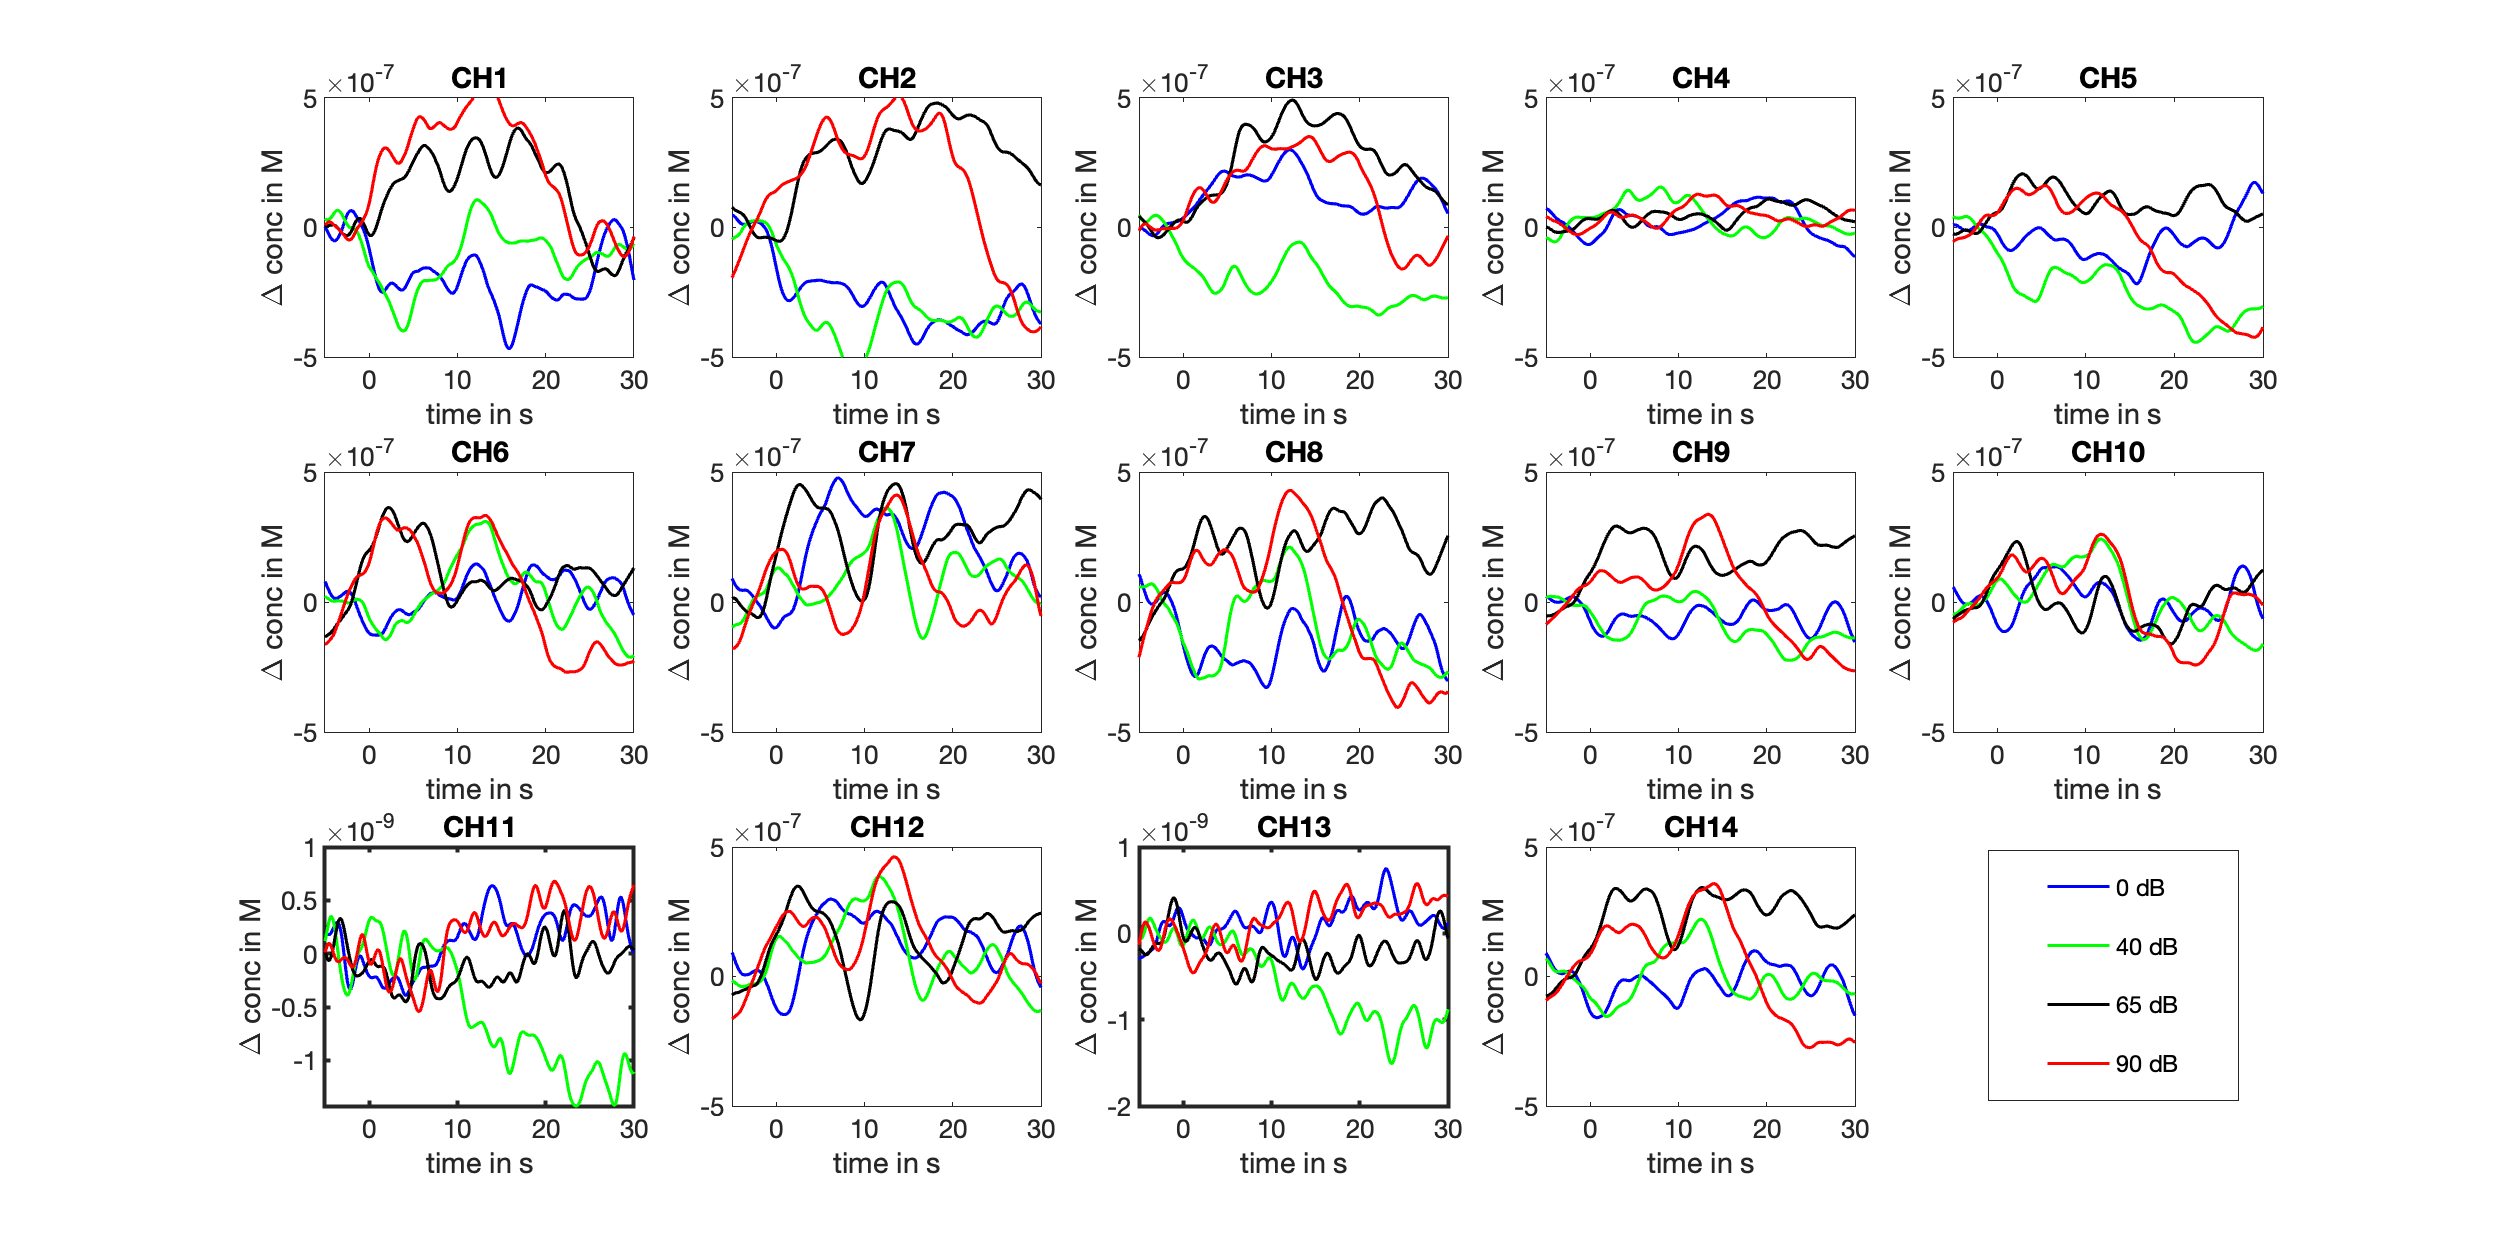
\includegraphics[scale=.4]{bilder/HbO_Mole/sub_chang_s_HbO.png}
  \caption{HbO measurement from participant 1.}
  \label{fig:somesignal}
  \medskip
  \footnotesize {Lines represent the block-averaged results over eight epochs. The averaged change of HbO concentration (in Mole) is plotted from 5 seconds before the start of the auditory stimuli to 30 seconds after the start of the stimuli. Four colours are used to differentiate the response from sound stimuli of different intensity levels.}
\end{figure}

\newpage

\begin{figure}[H]
  \centering
    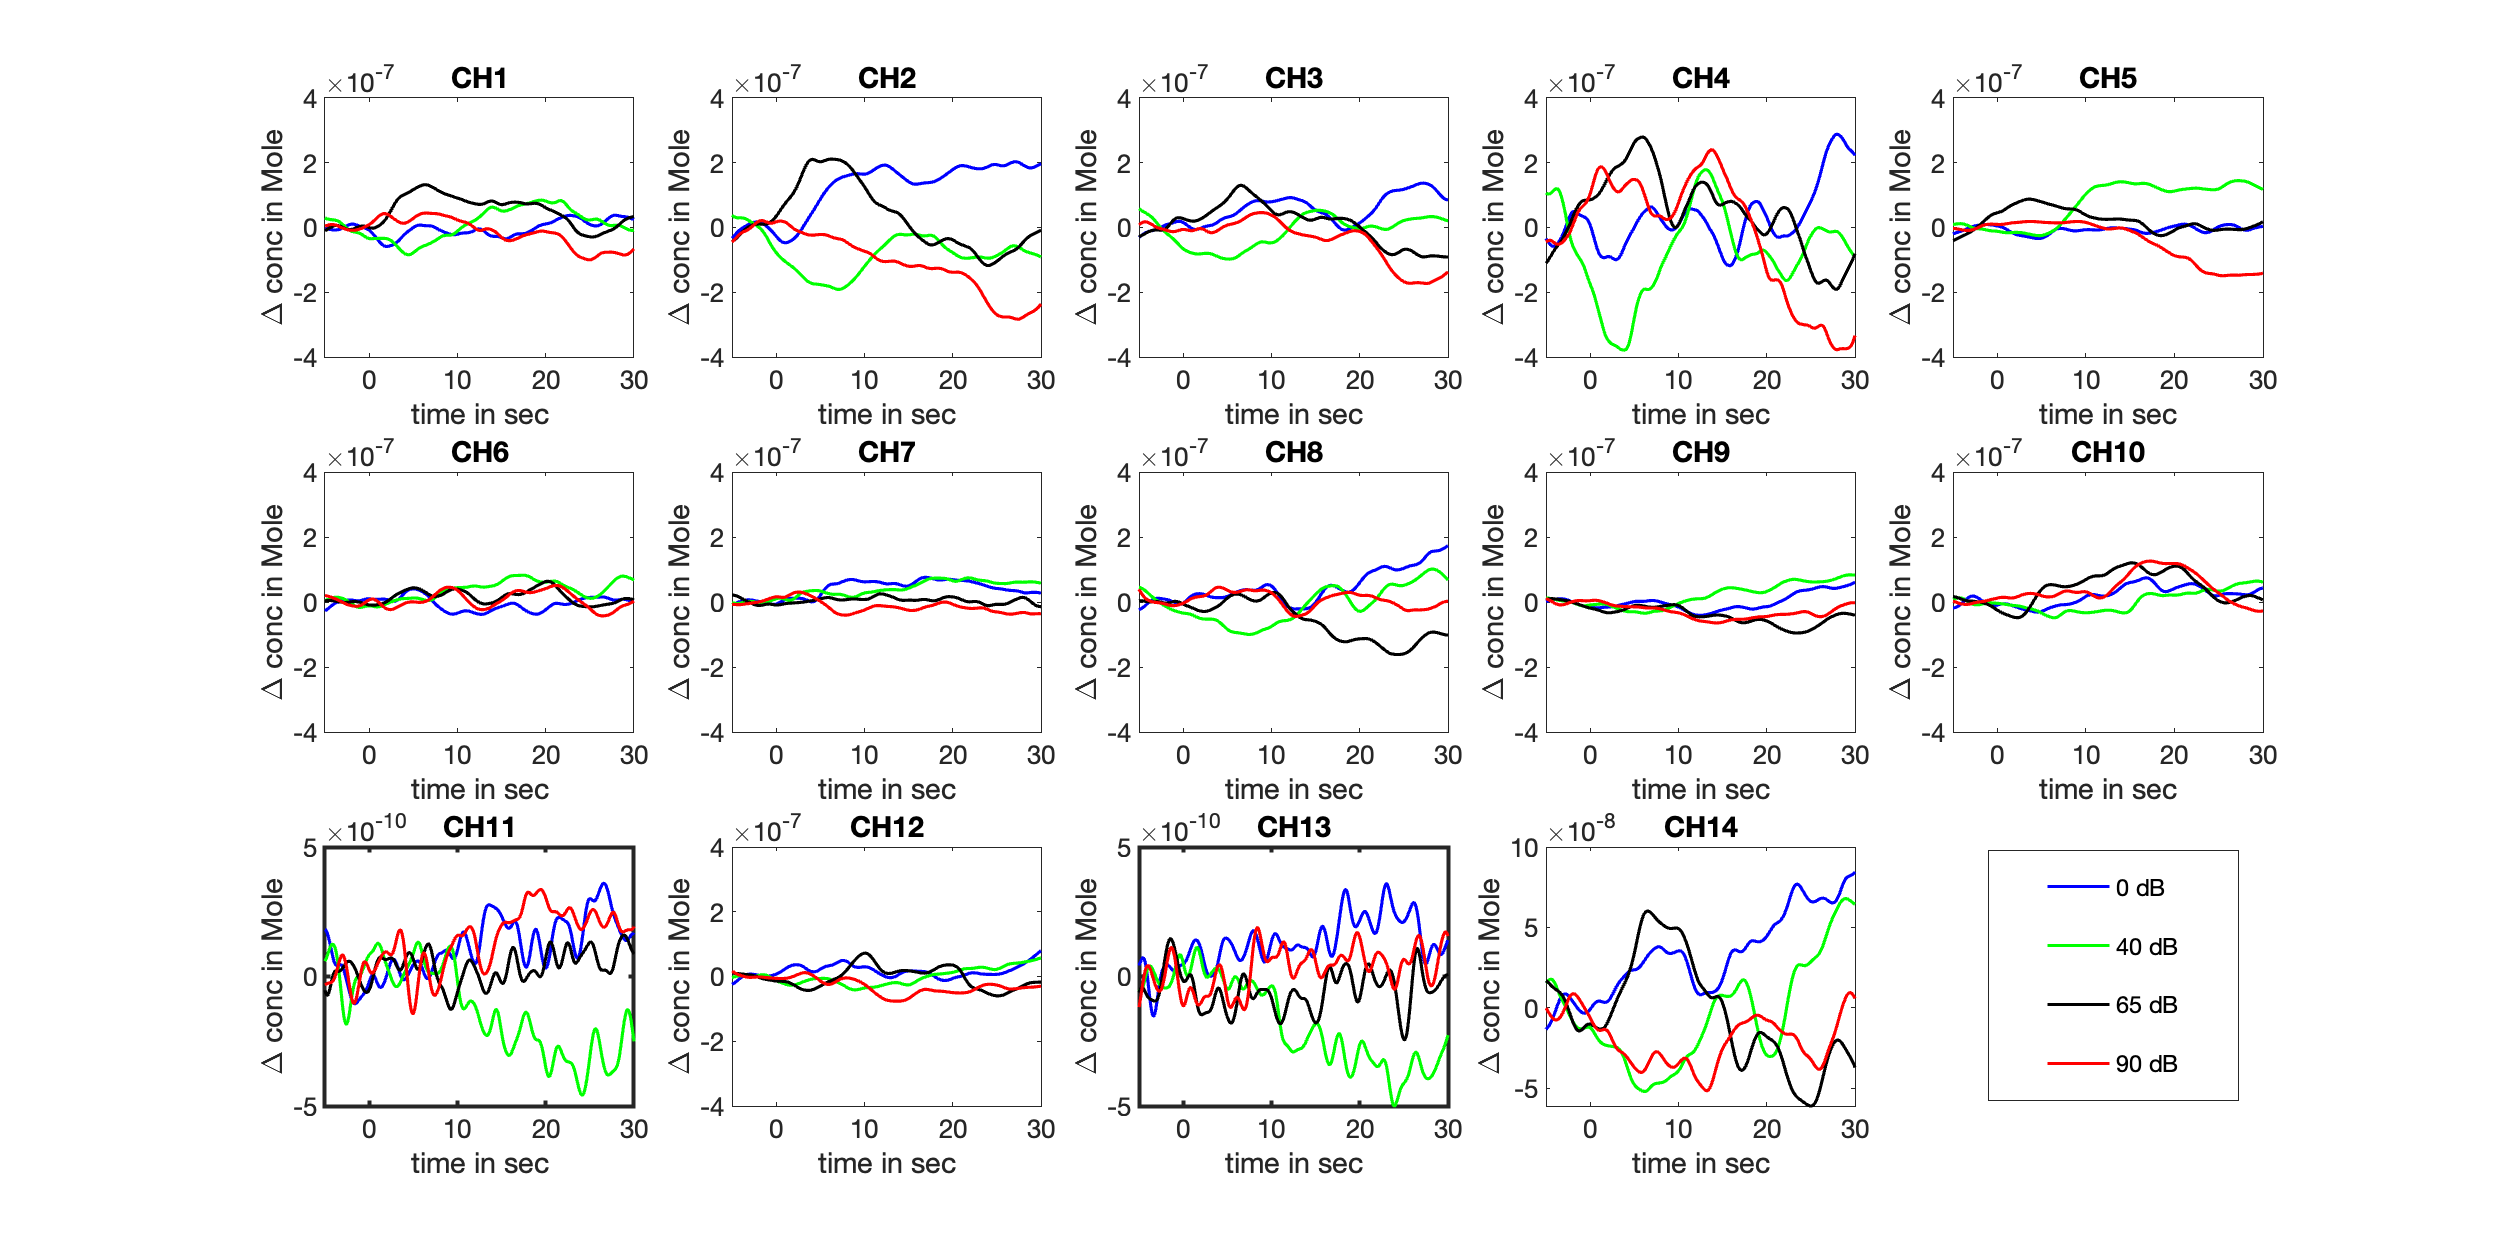
\includegraphics[scale=.4]{bilder/HbR_Mole/sub_chang_s_HbR.png}
  \caption{HbR measurement from participant 1.}
  \label{fig:somesignal}
  \medskip
  \footnotesize {Lines represent the block-averaged results over eight epochs. The averaged change of HbR concentration (in Mole) is plotted from 5 seconds before the start of the auditory stimuli to 30 seconds after the start of the stimuli. Four colours are used to differentiate the response from sound stimuli of different intensity levels.}
\end{figure}

\begin{figure}[H]
  \centering
    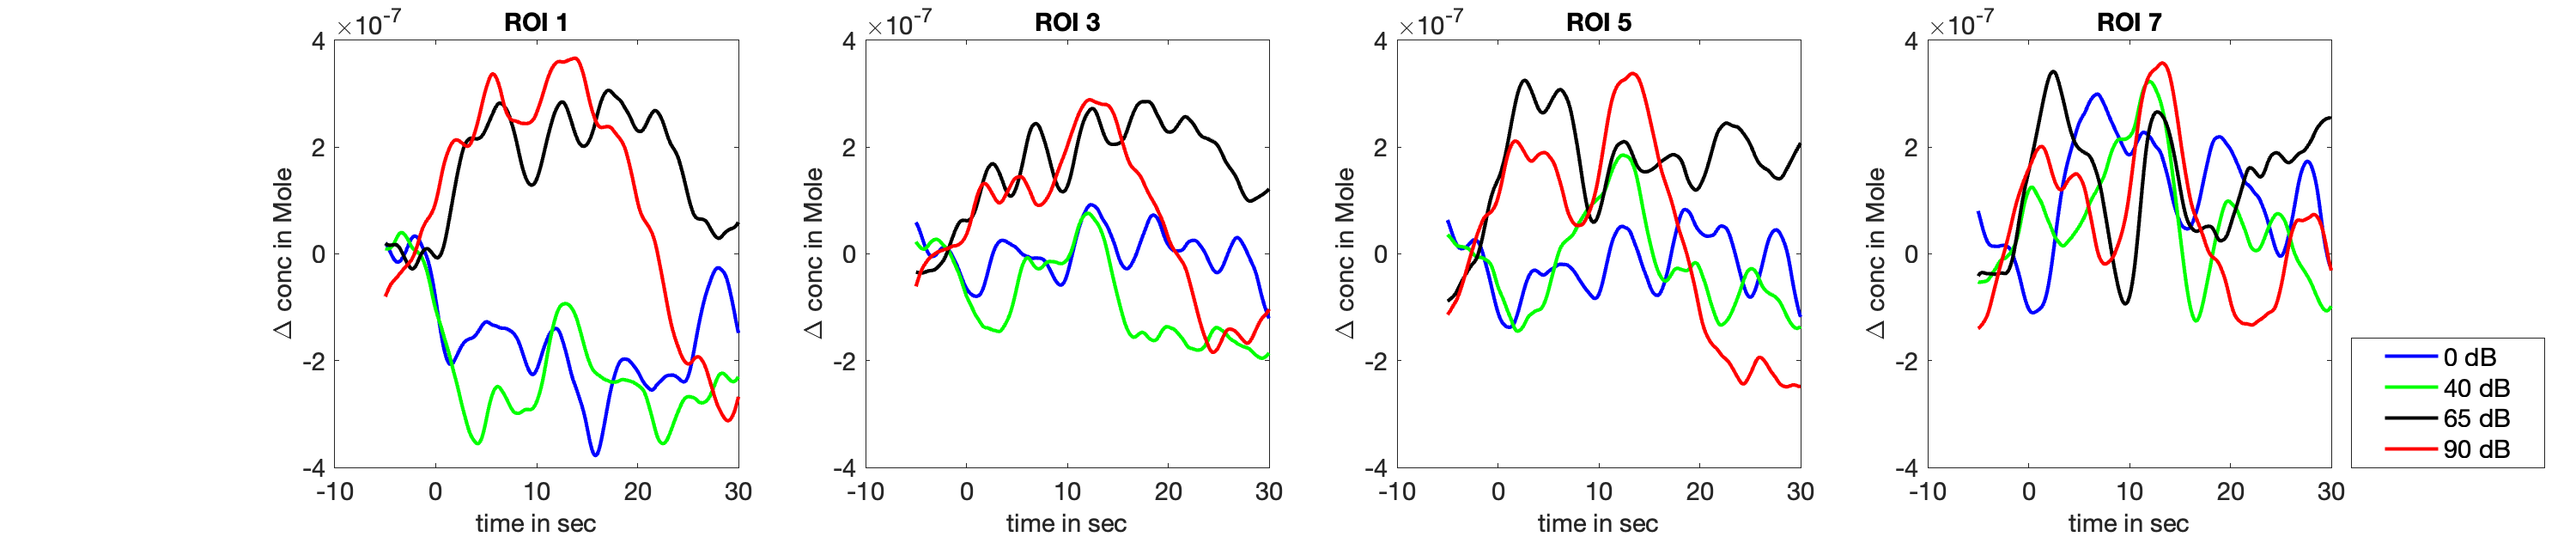
\includegraphics[scale=.29]{bilder/ROI/sub_chang_s_HbO.png}
  \caption{ROI measurement from participant 1.}
\end{figure}
\newpage


\section {Participant 2}

\begin{figure}[H]
  \centering
    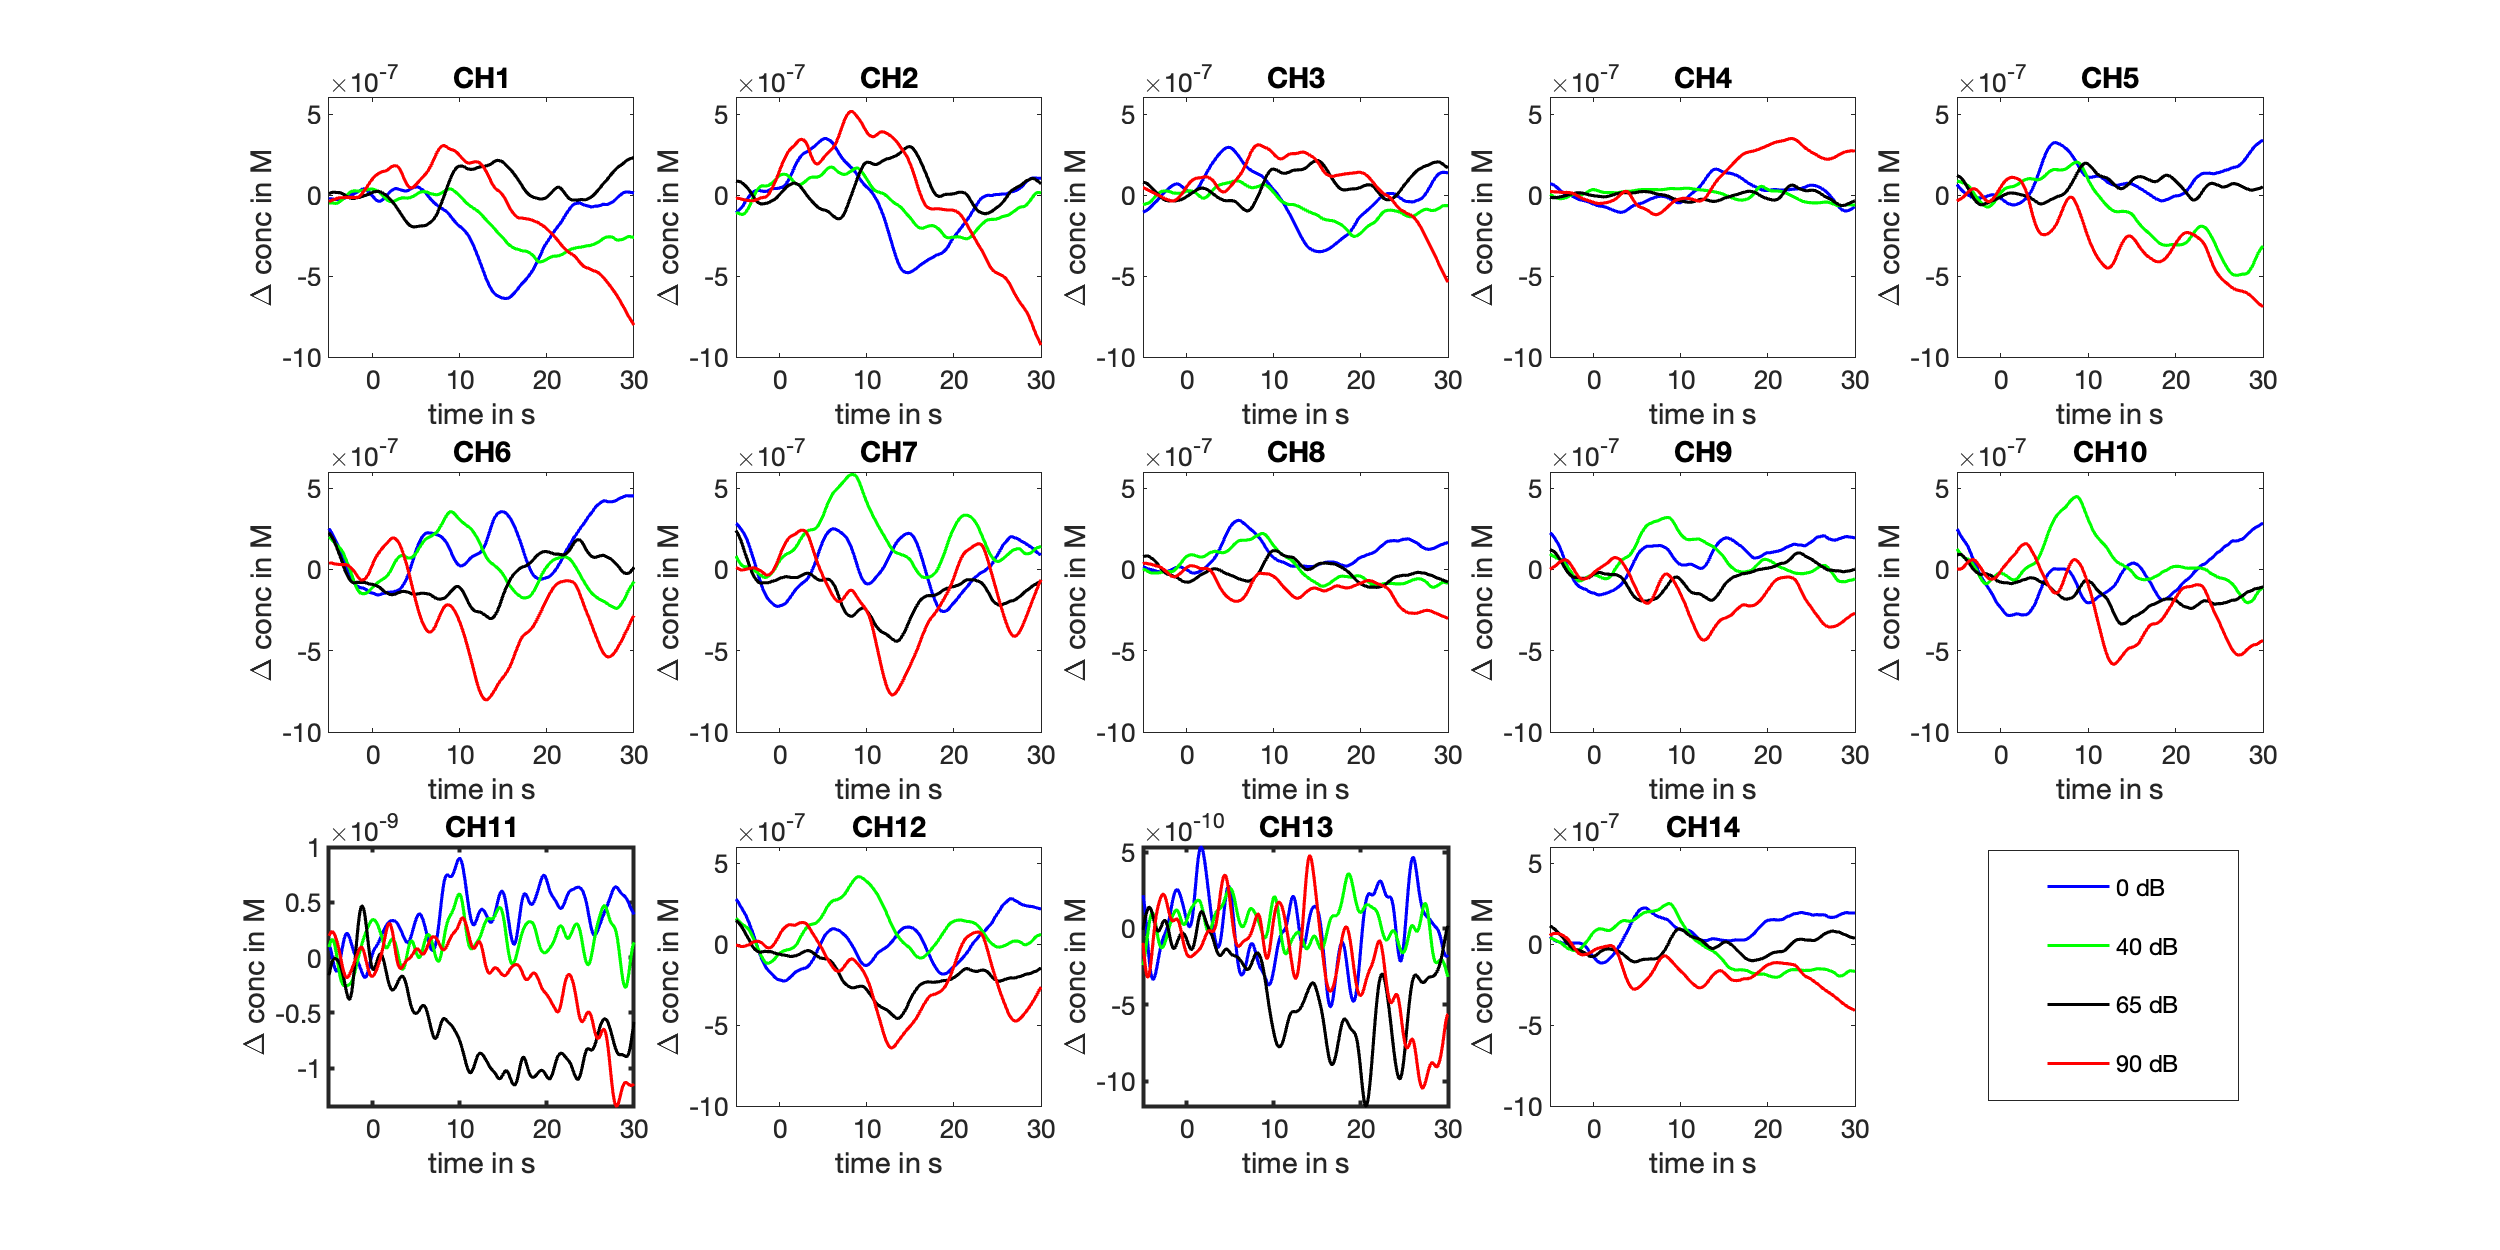
\includegraphics[scale=.4]{bilder/HbO_Mole/sub_gleb2_s_HbO.png}
  \caption{HbO measurement from participant 2.}
  \label{fig:somesignal}
  \medskip
  \footnotesize {Lines represent the block-averaged results over eight epochs. The averaged change of HbO concentration (in Mole) is plotted from 5 seconds before the start of the auditory stimuli to 30 seconds after the start of the stimuli. Four colours are used to differentiate the response from sound stimuli of different intensity levels.}
\end{figure}

\newpage

\begin{figure}[H]
  \centering
    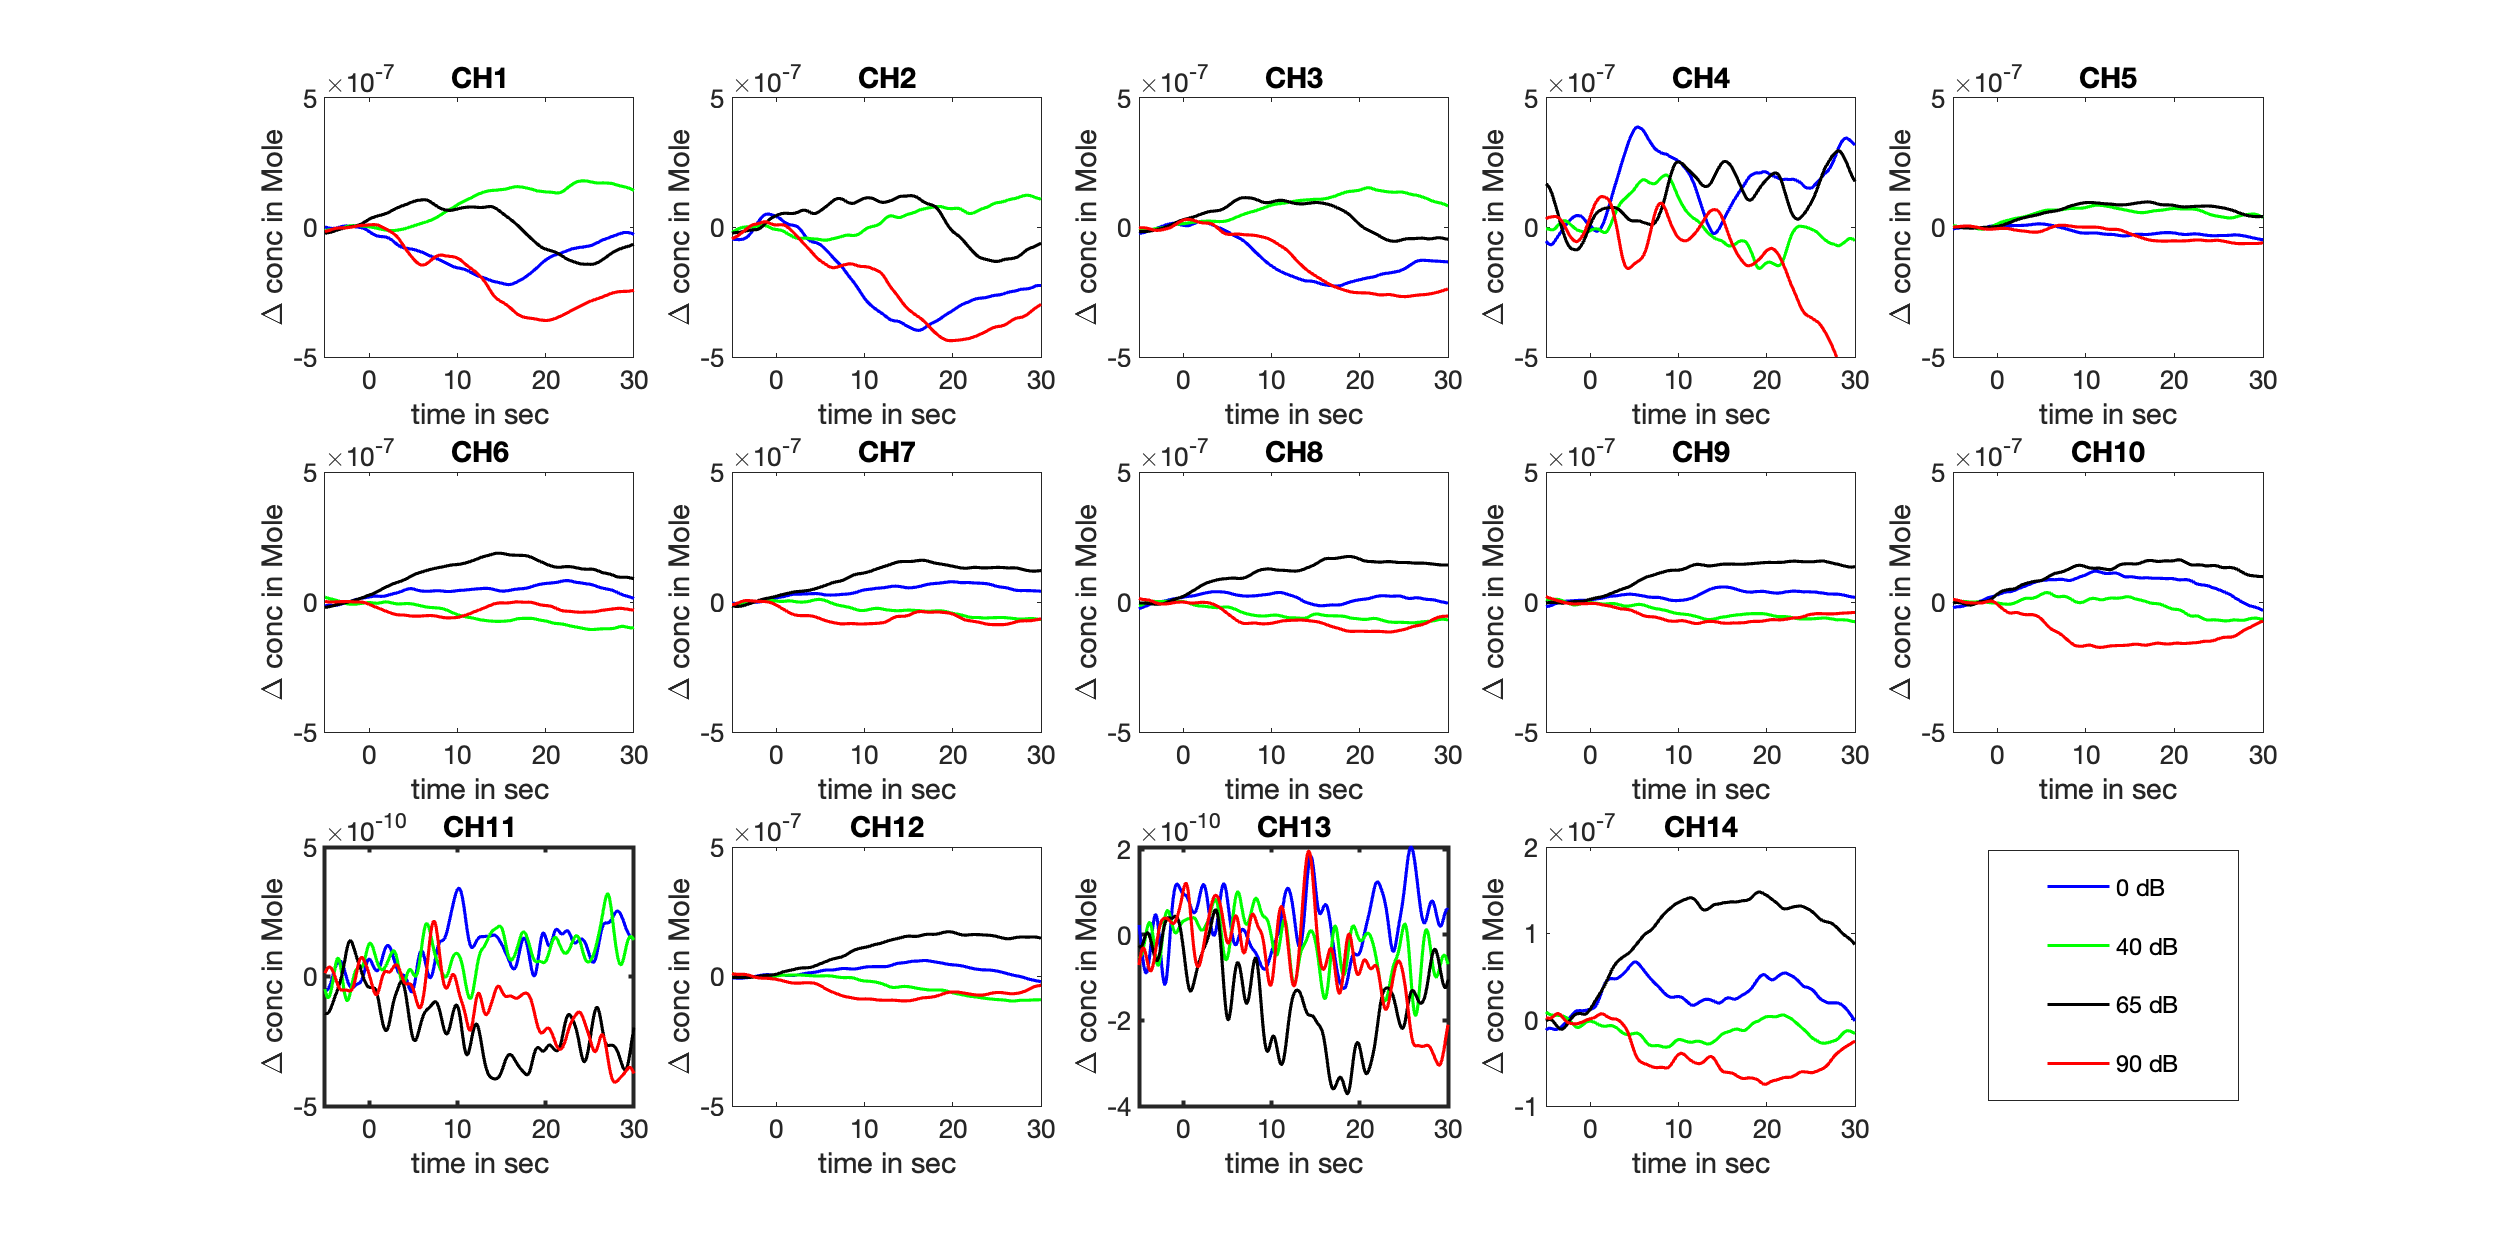
\includegraphics[scale=.4]{bilder/HbR_Mole/sub_gleb2_s_HbR.png}
  \caption{HbR measurement from participant 2.}
  \label{fig:somesignal}
  \medskip
  \footnotesize {Lines represent the block-averaged results over eight epochs. The averaged change of HbR concentration (in Mole) is plotted from 5 seconds before the start of the auditory stimuli to 30 seconds after the start of the stimuli. Four colours are used to differentiate the response from sound stimuli of different intensity levels.}
\end{figure}

\begin{figure}[H]
  \centering
    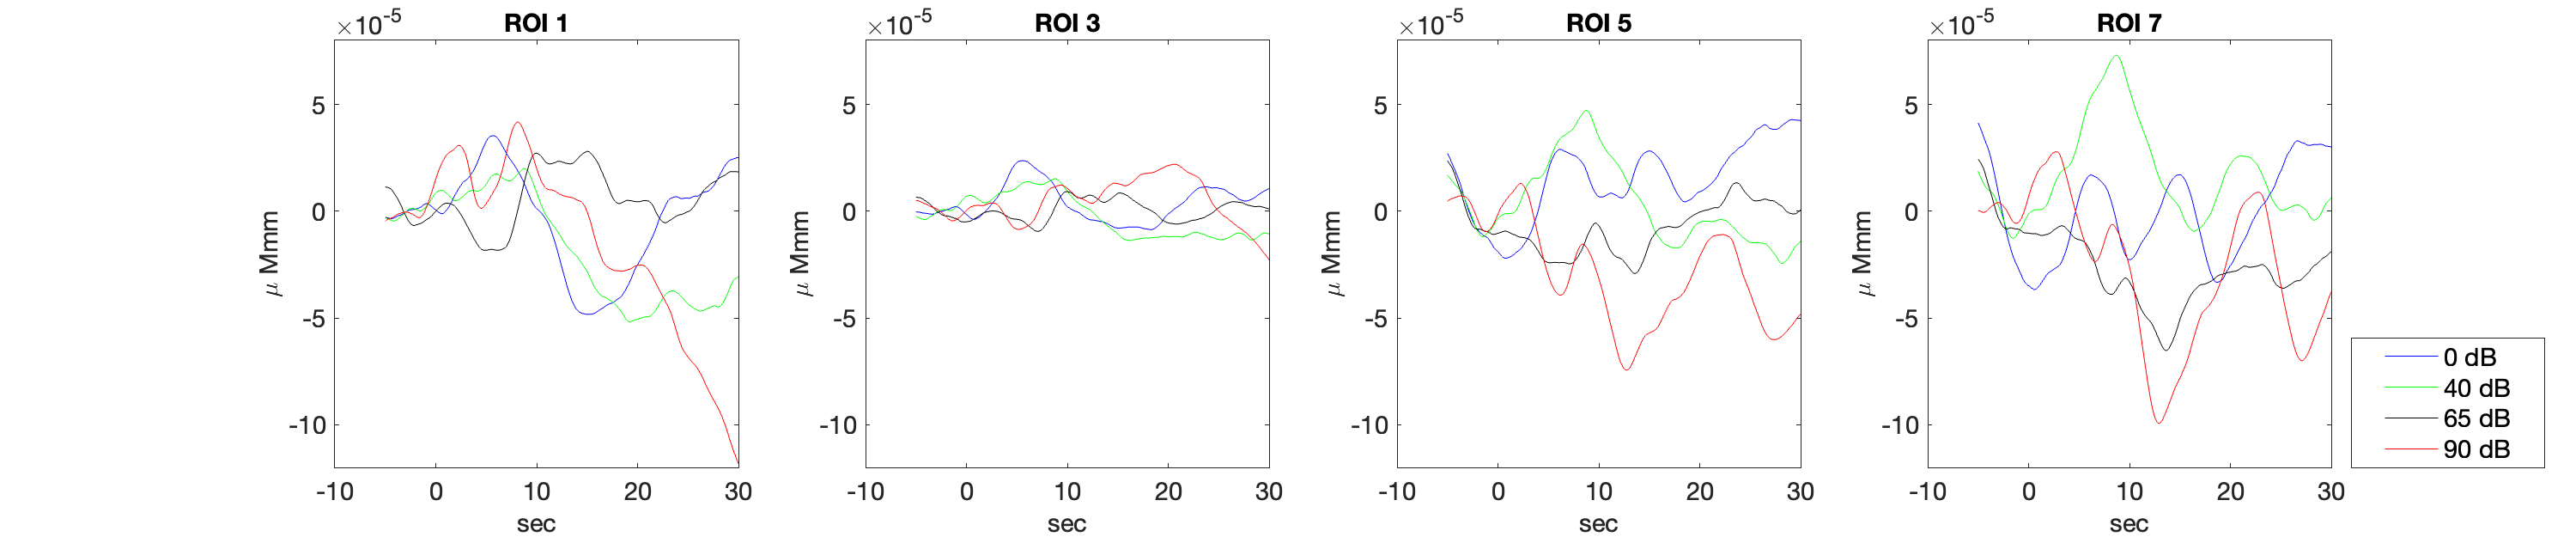
\includegraphics[scale=.29]{bilder/ROI/sub_gleb2_s_HbO.png}
  \caption{ROI measurement from participant 2.}
\end{figure}

\newpage

\section {Participant 6}
\begin{figure}[H]
  \centering
    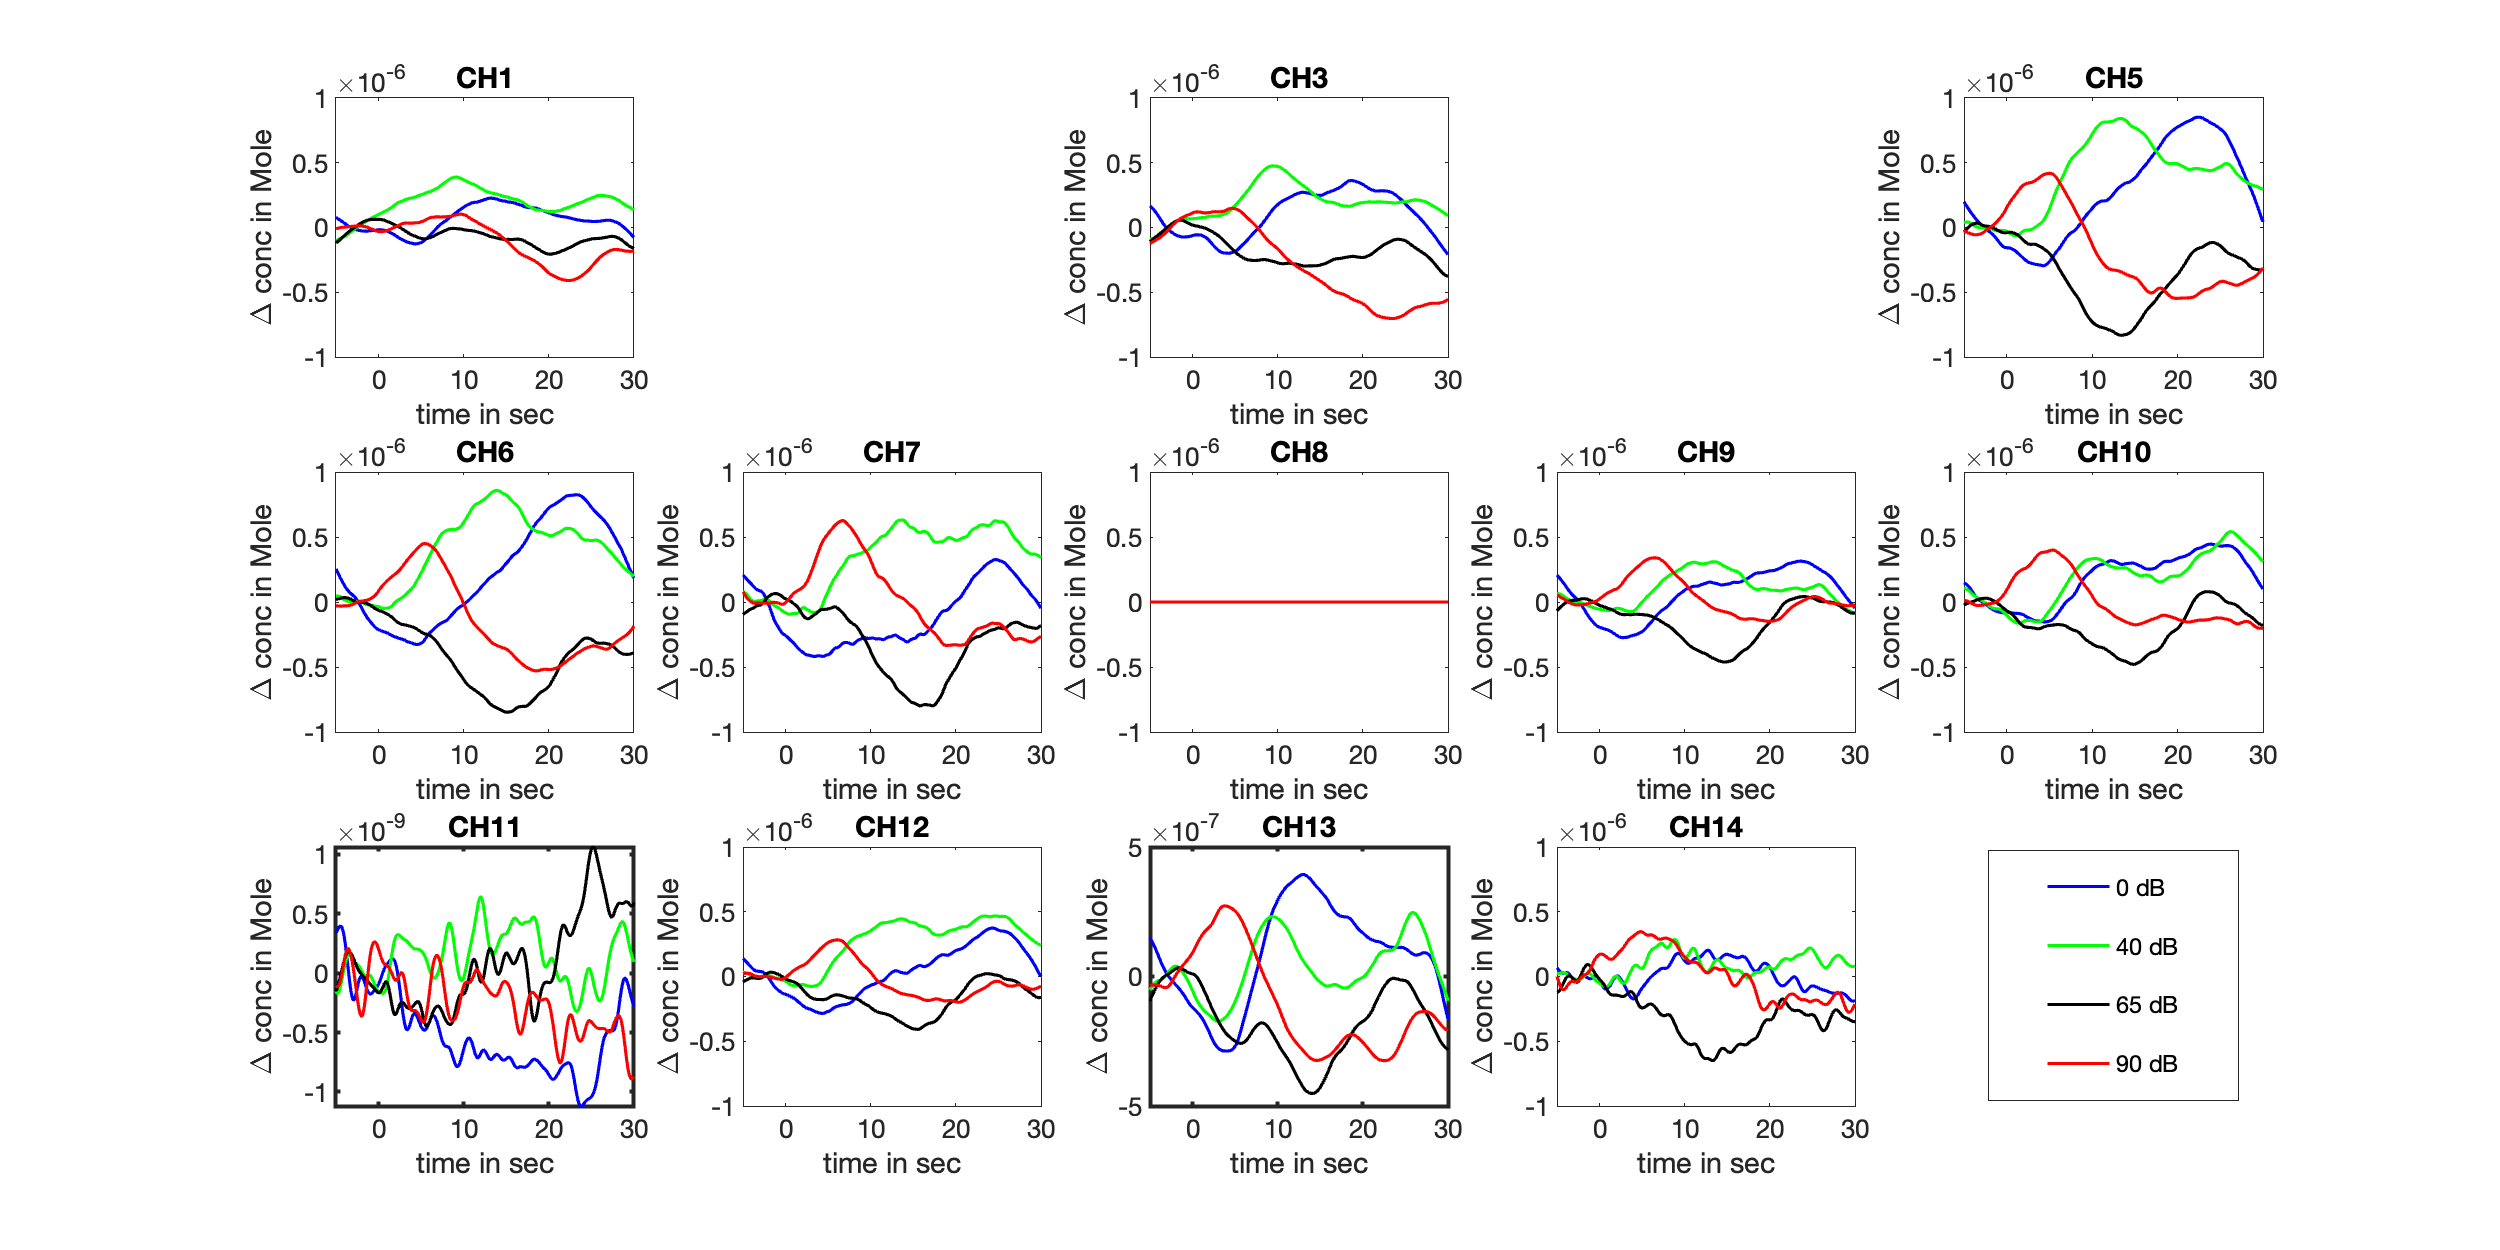
\includegraphics[scale=.4]{bilder/HbO_Mole/sub_shelia_s_HbO.png}
  \caption{HbO Measurement from participant 6.}
  \label{fig:somesignal}
  \medskip
  \footnotesize {Lines represent the block-averaged results over eight epochs. The averaged change of HbO concentration (in Mole) is plotted from 5 seconds before the start of the auditory stimuli to 30 seconds after the start of the stimuli. Four colours are used to differentiate the response from sound stimuli of different intensity levels.}
\end{figure}


\newpage


\begin{figure}[H]
  \centering
    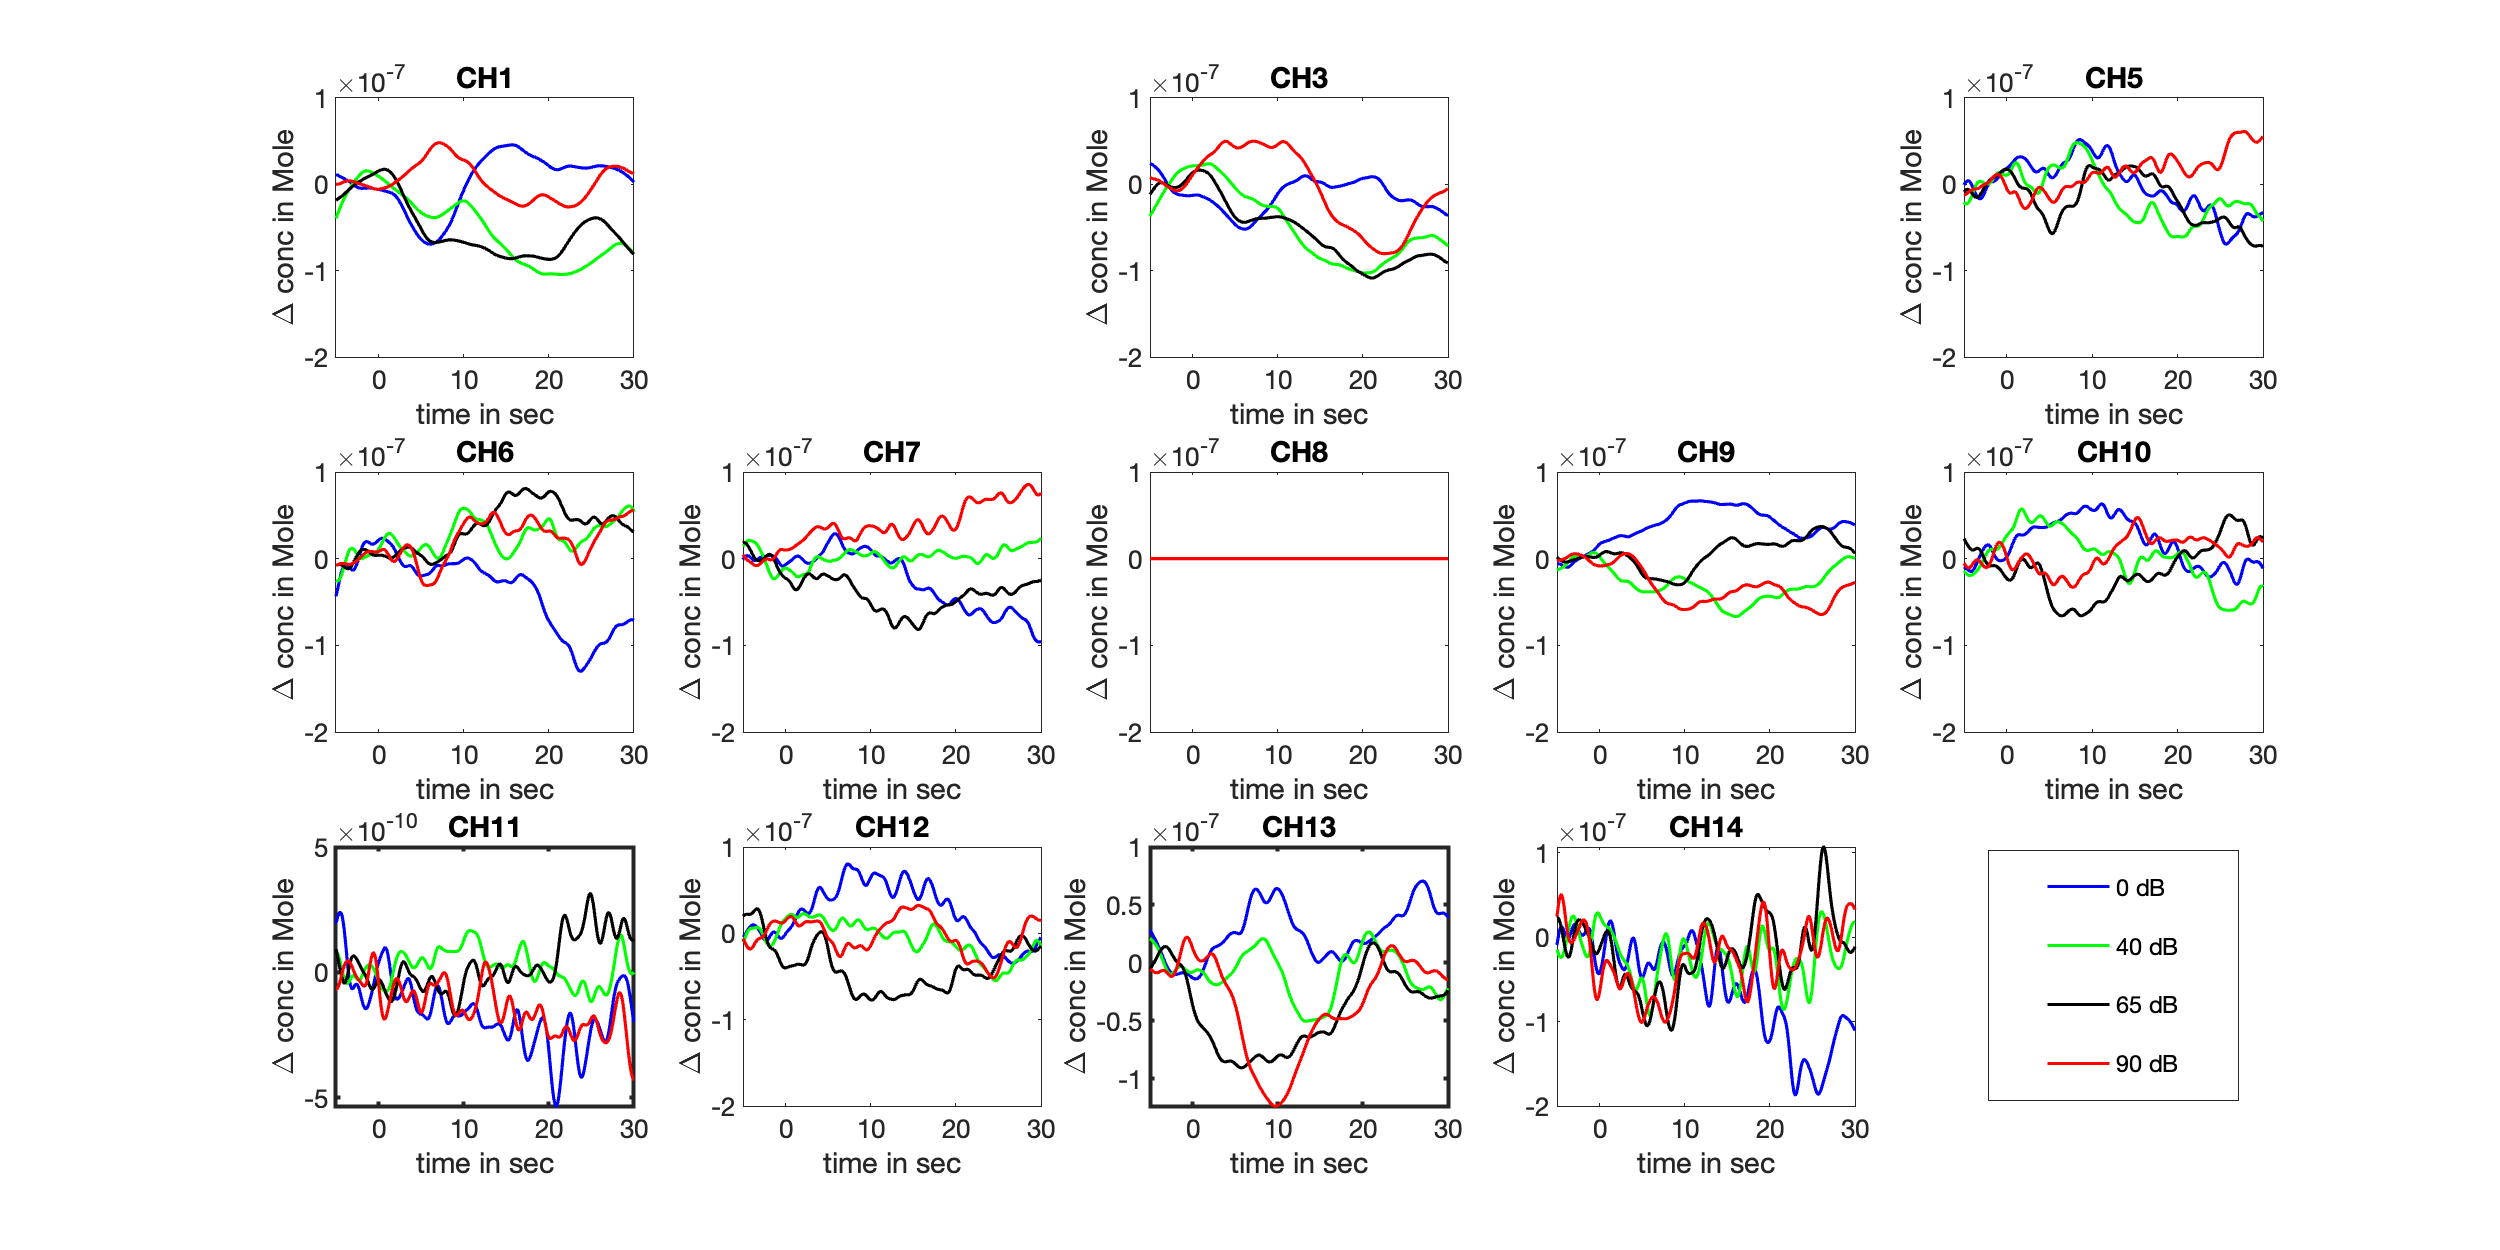
\includegraphics[scale=.4]{bilder/HbR_Mole/sub_shelia_s_HbR.png}
  \caption{HbR Measurement from participant 6.}
  \label{fig:somesignal}
  \medskip
  \footnotesize {Lines represent the block-averaged results over eight epochs. The averaged change of HbR concentration (in Mole) is plotted from 5 seconds before the start of the auditory stimuli to 30 seconds after the start of the stimuli. Four colours are used to differentiate the response from sound stimuli of different intensity levels.}
\end{figure}

\begin{figure}[H]
  \centering
    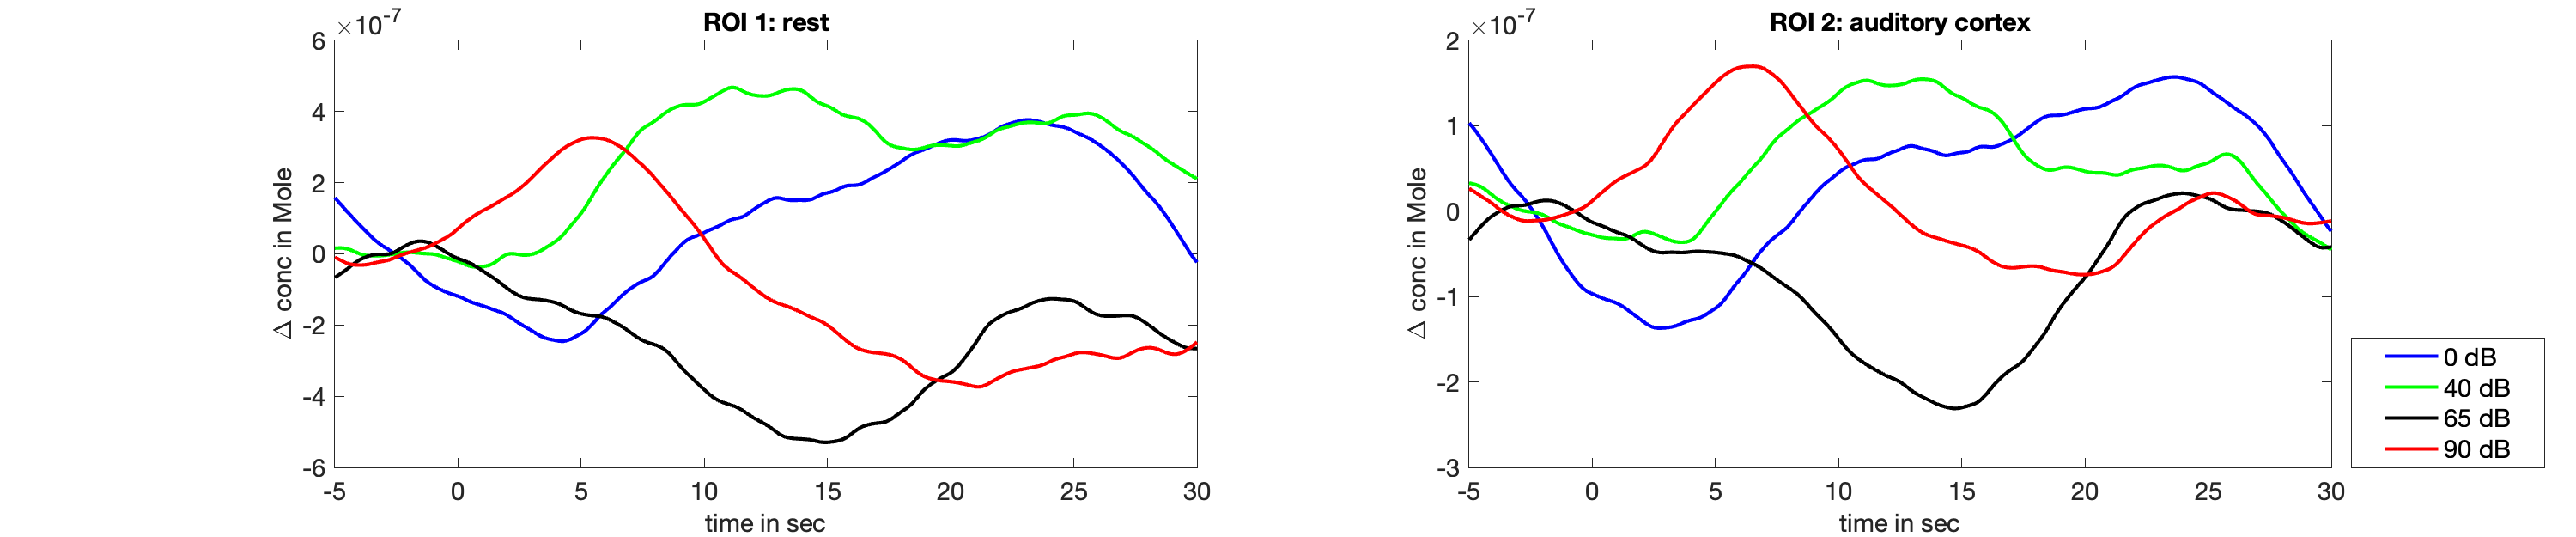
\includegraphics[scale=.29]{bilder/ROI/sub_shelia_s_HbO.png}
  \caption{ROI Measurement from participant  6.}
\end{figure}

For the oxygenated hemoglobin, \acrshort{HbO} waveform, the loudest sound stimuli resulted in phasic response for almost all the channels. In addition, it also resulted in faster on-set compared with other stimuli of lower sound pressure levels.

On the other hand, as for the deoxygenated hemoglobin, \acrshort{HbR} response, results from multiple channels appeared to be noisy even if the SCI values were already above the suggested threshold.

\newpage

\section {Participant 8}

\begin{figure}[H]
  \centering
    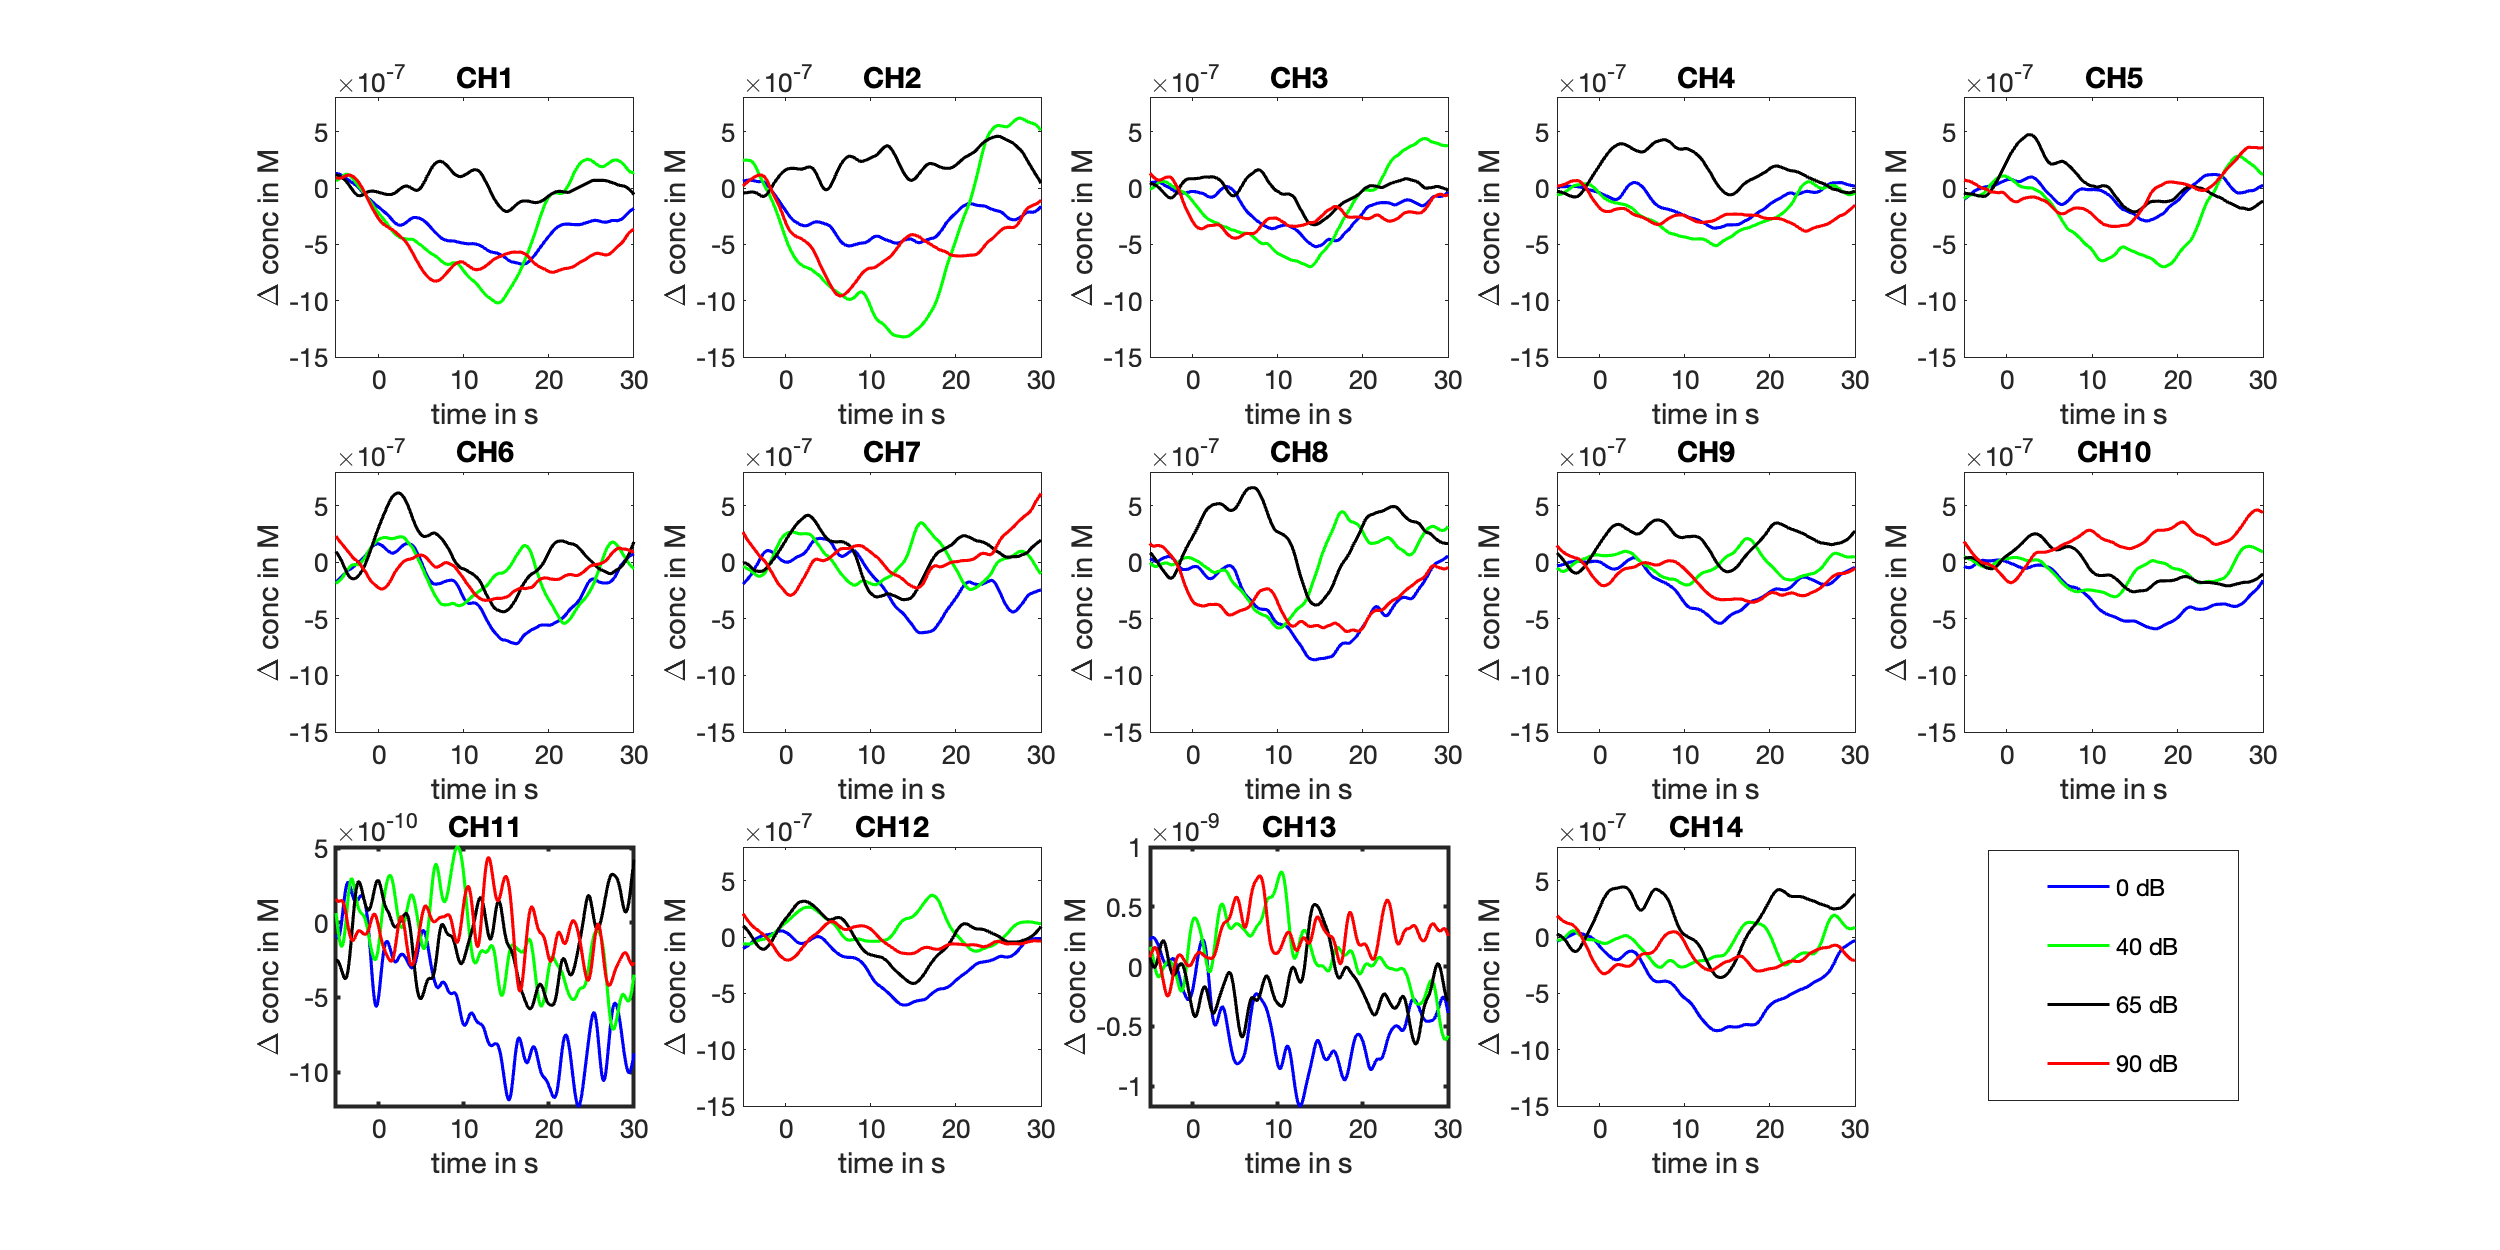
\includegraphics[scale=.4]{bilder/HbO_Mole/sub_luca2_s_HbO.png}
  \caption{HbO measurement from participant 8. Silent comparison}
  \label{fig:somesignal}
  \medskip
  \footnotesize {Lines represent the block-averaged results over eight epochs. The averaged change of HbO concentration (in Mole) is plotted from 5 seconds before the start of the auditory stimuli to 30 seconds after the start of the stimuli.}
\end{figure}

\newpage

\begin{figure}[H]
  \centering
    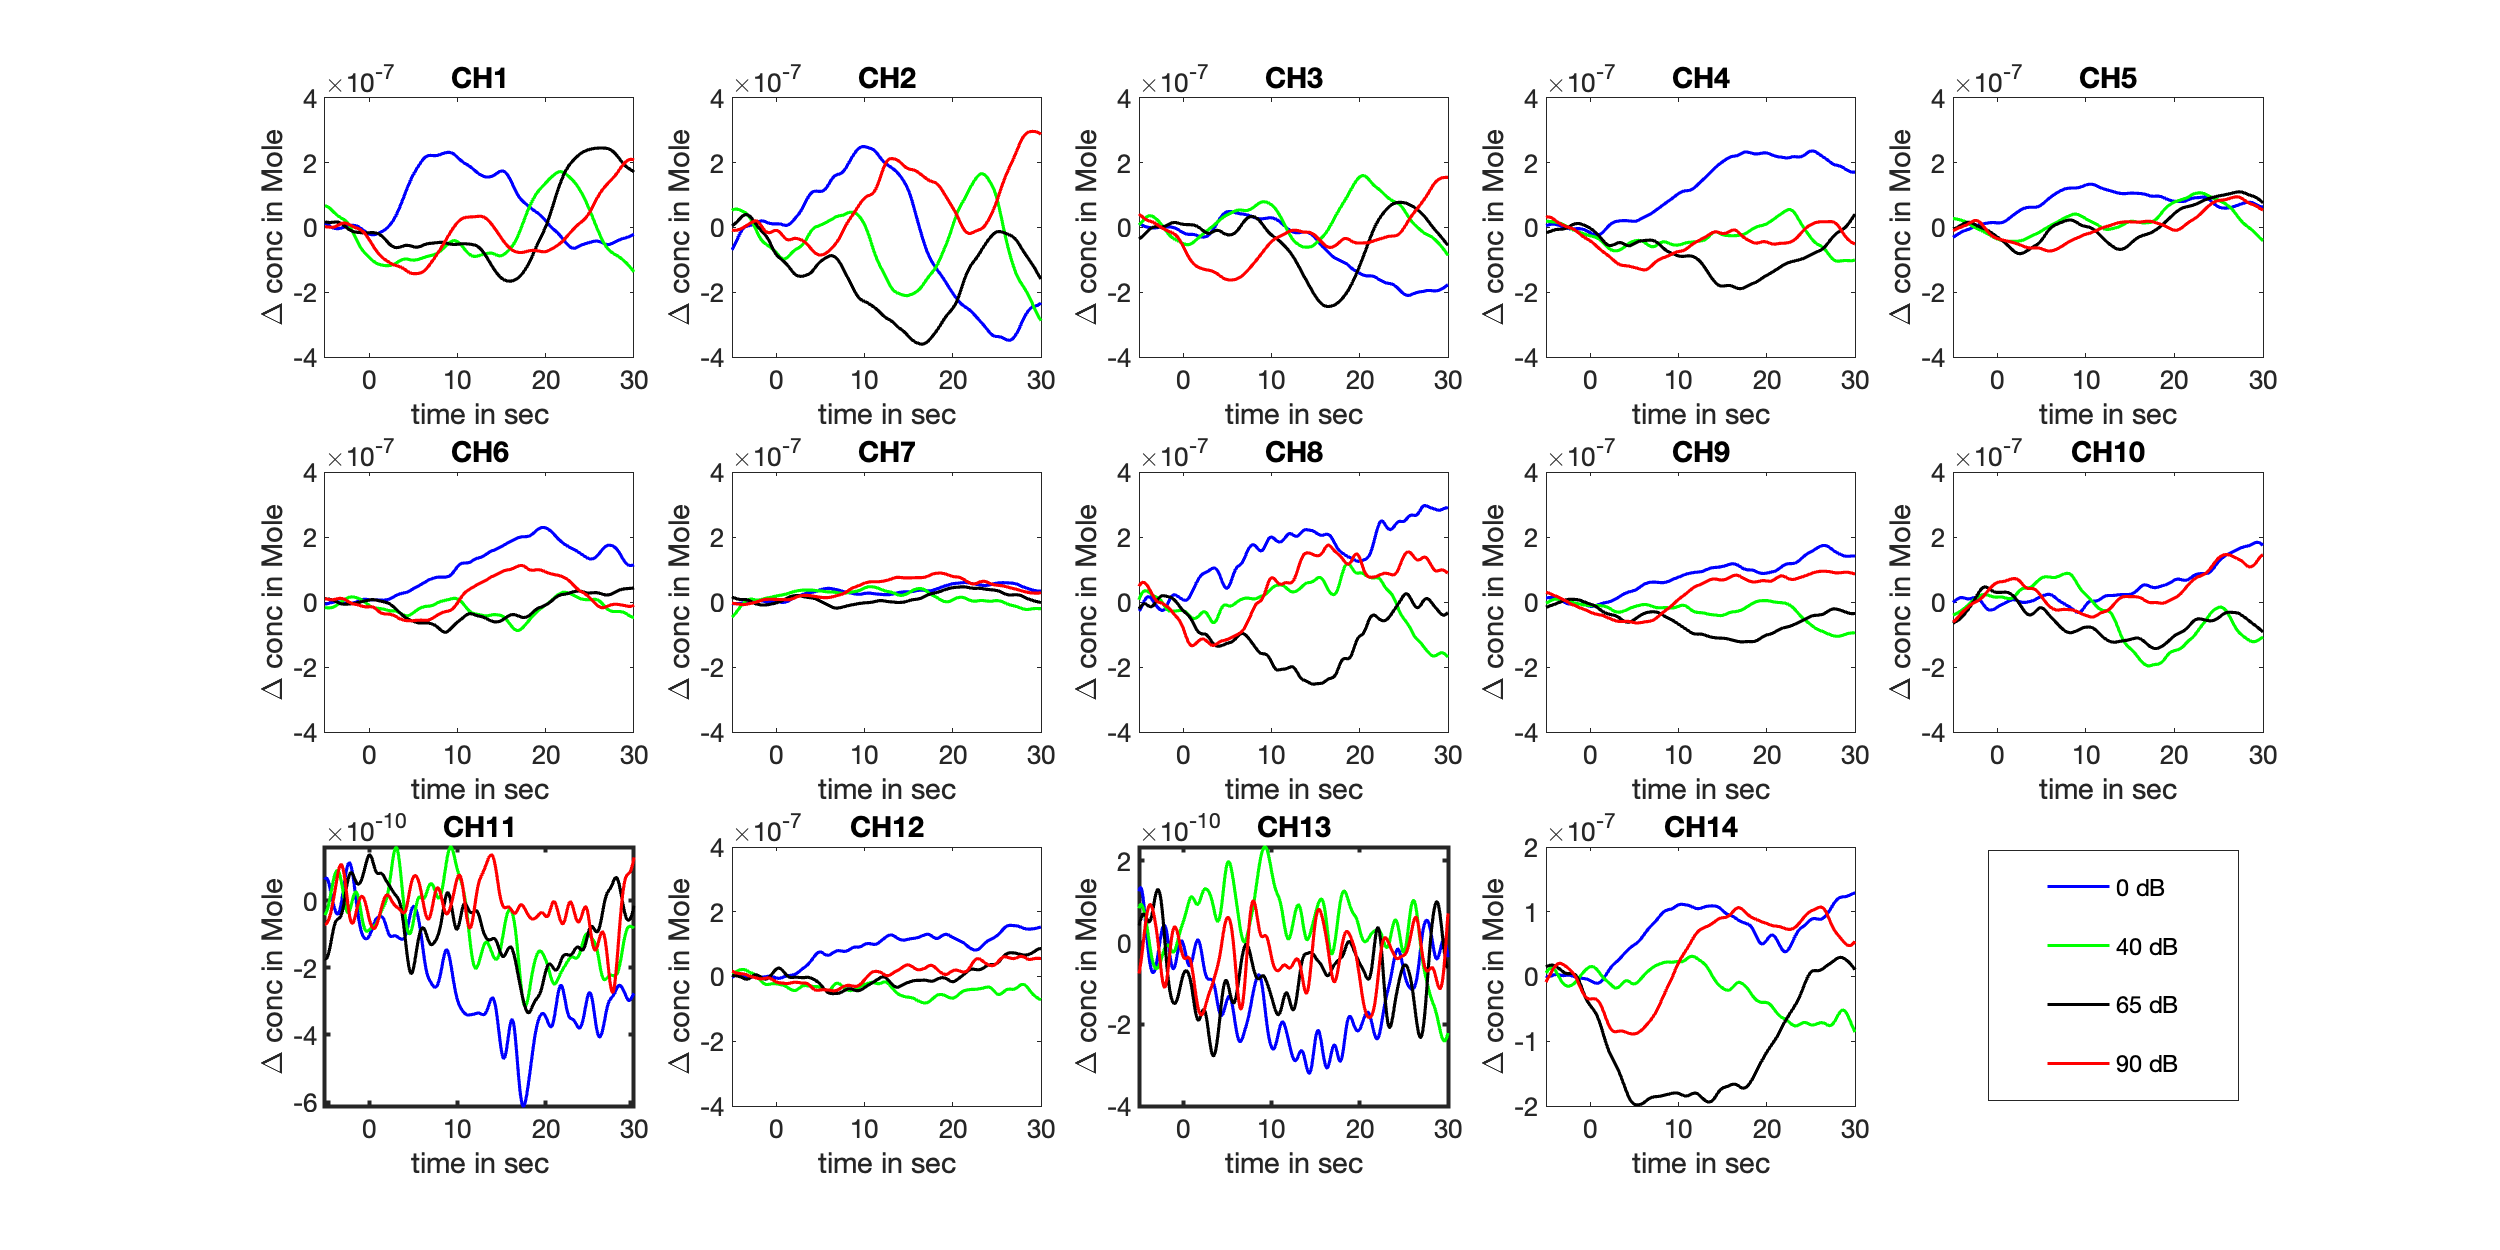
\includegraphics[scale=.4]{bilder/HbR_Mole/sub_luca2_s_HbR.png}
  \caption{HbR measurement from participant 8. Silent comparison}
  \medskip
  \footnotesize {Lines represent the block-averaged results over eight epochs. The averaged change of HbR concentration (in Mole) is plotted from 5 seconds before the start of the auditory stimuli to 30 seconds after the start of the stimuli.}
\end{figure}

\begin{figure}[H]
  \centering
    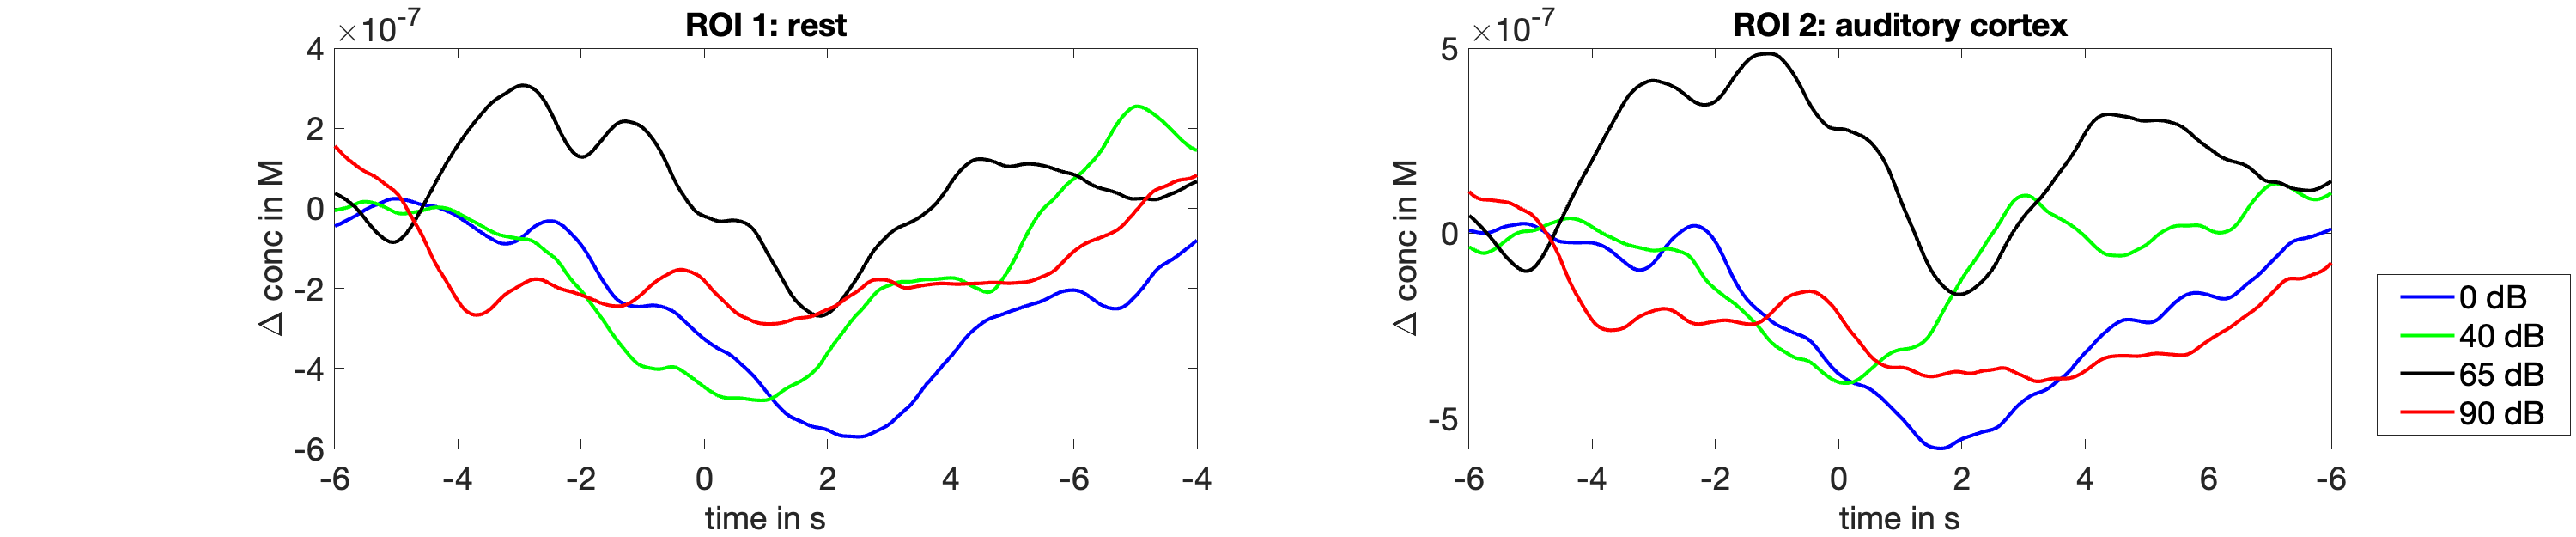
\includegraphics[scale=.29]{bilder/ROI/sub_luca2_s_HbO.png}
  \caption{ROI measurement from participant 8. Silent comparision.}
\end{figure}

This participant was given only silence stimuli. No pattern could be concluded for the measured waveform morphology. Nonetheless, it is noteworthy to know that even if there were almost no visual and sound stimuli, dynamic hemoglobin response still presented.


%%% Bibliography
\bibliographystyle{apalike}
%\bibliographystyle{plain}
\setcitestyle{authoryear,open={((},close={))}}
\bibliography{other/citation}
\nocite{*}
\addcontentsline{toc}{chapter}{\refname}
\cleardoublepage{}


%%% Erklaerung der Selbststaendigkeit
\erklaerung{}


\end{document}
